\chapter{Legolas applications} \label{ch: legolas_applications}


\graphicspath{{05-applying_legolas/figures/}}

\begin{chapterquote}[Robert C. Martin][Clean Code: A Handbook of Agile Software Craftsmanship][]
  Why do most developers fear to make continuous changes to their code? Because they are afraid they'll break it.
  Why are they afraid they'll break it? Because they don't have tests.
\end{chapterquote}

\usespublishedwork{
  Most of this Chapter was published in ``Legolas: a novel tool for magnetohydrodynamic spectroscopy'', 2020, \apjs,
  251, 25 \citep{claes2020_legolas}. N. Claes developed {\legolas} in close collaboration with J. De Jonghe, generated the data and figures and wrote a first draft of the manuscript; J. De Jonghe revised and extended the manuscript. R. Keppens contributed to the revision of the paper.
}

In the previous Chapter we discussed the mathematical formalism behind {\legolas}. As is common practice when developing a brand new numerical code we now have to test the implementation against various known results. This Chapter will mostly be dedicated to the validation of our new numerical tool, by comparing numerical spectra with known results from theory and/or the literature. Additionally, we will briefly touch upon the extensive (and continuous) testing framework {\legolas} uses.

\section{Introduction}
Any piece of software, both existing and newly developed, should be accompanied by a decent testing framework to ensure that any changes made to the code, either in the present or in the future, do not break things that were previously working fine. It is easy to develop a piece of code, it is less easy to develop a \emph{working} piece of code, and finally it is certainly not enough for code to just ``work''. Every part of the implementation should be tested against known results in order to make sure that the code actually does what it is expected to do. In an ideal world, every single line of a code base is tested at least once, while at the same time also accounting for various branches in the logic.

In this Chapter we validate {\legolas} against a plethora of test cases, thereby ensuring a correct treatment of the governing equations. Depending on which physical effects are taken into account, we know a priori some general spectral properties that should hold, and we can thus test the properties of the obtained spectra against our predictions. For eigenmode quantifications of ideal, static MHD configurations under adiabatic conditions, we know that the static -- that is, no equilibrium flow -- and adiabatic linear MHD equations make the problem self-adjoint. When performing a standard Fourier analysis in the ignorable directions, the resulting eigenvalue problem is then Hermitian, meaning that all eigenfrequencies will be either fully real (stable waves) or fully complex (pure damped or unstable modes), hence they are found on the real or imaginary axis of the complex eigenfrequency plane, and the full MHD spectrum will be both left-right and up-down symmetric. The inclusion of nonideal effects like resistivity or thermal conduction lifts the self-adjointness of the eigenvalue problem, allowing the eigenmodes to move away from the axes into the complex plane, and the up-down symmetry gets broken. As long as the equilibrium configuration is static, all (adiabatic or non-adiabatic) modes will still have a complementary mode that lies mirrored around the imaginary axis, making the entire spectrum left-right symmetric. This is related to the forward and backward propagating mode symmetry, or the equivalent statement on the parity-time (PT) symmetry.

The inclusion of a background flow breaks the left-right symmetry of the MHD spectrum, resulting in an even more complicated spectral structure. However, the study of the ideal, linear MHD spectrum of flowing plasmas is still governed by a pair of self-adjoint operators \citep{goedbloed2011,book_MHD}, and it leaves the up-down symmetry of the spectrum intact (where every overstable mode has an equivalent damped counterpart at the same frequency).

The actual validation of the code should follow a stepwise approach, where we first test the most simple cases. This is dictated by common logic: if even the most simple cases do not work, then we can never expect correct spectra for more complicated equilibria. Hence to begin with, we discuss results for adiabatic equilibria where only gravity is included. In this case we can compare numerical spectra obtained through {\legolas} with analytical solutions acquired by solving dispersion relations; here, we first focus on stratified atmospheres containing $p$ and $g$ modes. We then move on to cylindrical geometries, where we first look at adiabatic flux tubes, followed by the inclusion of flow effects by considering equilibria known to be susceptible to KHI and Suydam cluster modes. Next, our focus shifts to nonadiabatic effects by looking at a resistive MHD calculation for a case without gravity, where the value of a quasi-mode is known analytically. Resistive tearing modes are also discussed, combining the effects of flow and resistivity. Finally we will treat the inclusion of thermal conduction and optically thin radiative cooling effects, where we look at nonadiabatic discrete Alfv\'en waves and magnetothermal modes.


\section{Cartesian cases: waves in stratified atmospheres}
First of all we discuss multiple theoretical results for adiabatic equilibria in a Cartesian geometry, where only gravity is included. We consider $p$ and $g$ odes in stratified layers and pay special attention to specific unstable branches.

\subsection{Gravito-MHD waves} \label{ss: gravito-mhd}
The first test case covers gravito-MHD waves as discussed in \citet[Figure 7.9]{book_MHD}, which handles an exponentially stratified atmosphere with constant sound and Alfv\'en speeds. This magnetised atmosphere contains the generalisation of the $p$ and $g$ modes of an unmagnetised layer, and the constancy of the sound and Alfv\'en speed renders this particular configuration analytically tractable (even though it has an inhomogeneous density profile), because the slow and Alfv\'en continua collapse to points. the geometry is Cartesian with $x \in [0, 1]$ and an equilibrium configuration given by
\begin{equation} \label{eq: gravito_mhd}
  \begin{gathered}
    \rho_0 = \rho_c \exp\left(-\alpha x\right), \qquad p_0 = p_c \exp\left(-\alpha x\right), \\
    \bb_0 = B_c \exp\left(-\frac{1}{2}\alpha x\right)\unit{z}, \qquad \alpha = \frac{\rho_c g}{p_c + \frac{1}{2}B_c},
  \end{gathered}
\end{equation}
where $p_c$ and $B_c$ are taken to be 0.5 and 1, respectively, as to yield a plasma beta equal to unity. The parameter $\alpha$ is taken to be 20, which, together with $g = 20$, is used to constrain the value for the constant $\rho_c$. These four equations completely determine the equilibrium configuration, because the temperature is $T_0 = p_0/\rho_0$, following the ideal gas law. The spectrum discussed in \citet{book_MHD} is actually the solution to the analytic dispersion relation for gravito-MHD waves, which shows the squared eigenvalue as a function of wavenumber for a fixed angle $\theta = \pi / 4$ between the wave vector $\bk_0$ and the magnetic field $\bb_0$. However, the spectrum as calculated by {\legolas} corresponds to one single equilibrium configuration, meaning one value for $k_y$ and $k_z$. In order to reproduce Figure 7.9 from \citet{book_MHD} and compare the results, we performed 100 different runs where the equilibrium parameters in Equation \eqref{eq: gravito_mhd} remained unchanged, but $k_y$ and $k_z$ took on 100 different values between $0$ and $\sqrt{250}$ as to yield a wavenumber range for $k_0^2$ between 0 and 500. Because the magnetic field is purely aligned with the $z$-axis, we can write $\kpara = k_z = k_0\cos(\theta)$ and $\kperp = k_y = k_0\sin(\theta)$. All runs were performed using 351 gridpoints, yielding a matrix size of $5616 \times 5616$.

\begin{figure}[t]
  \centering
  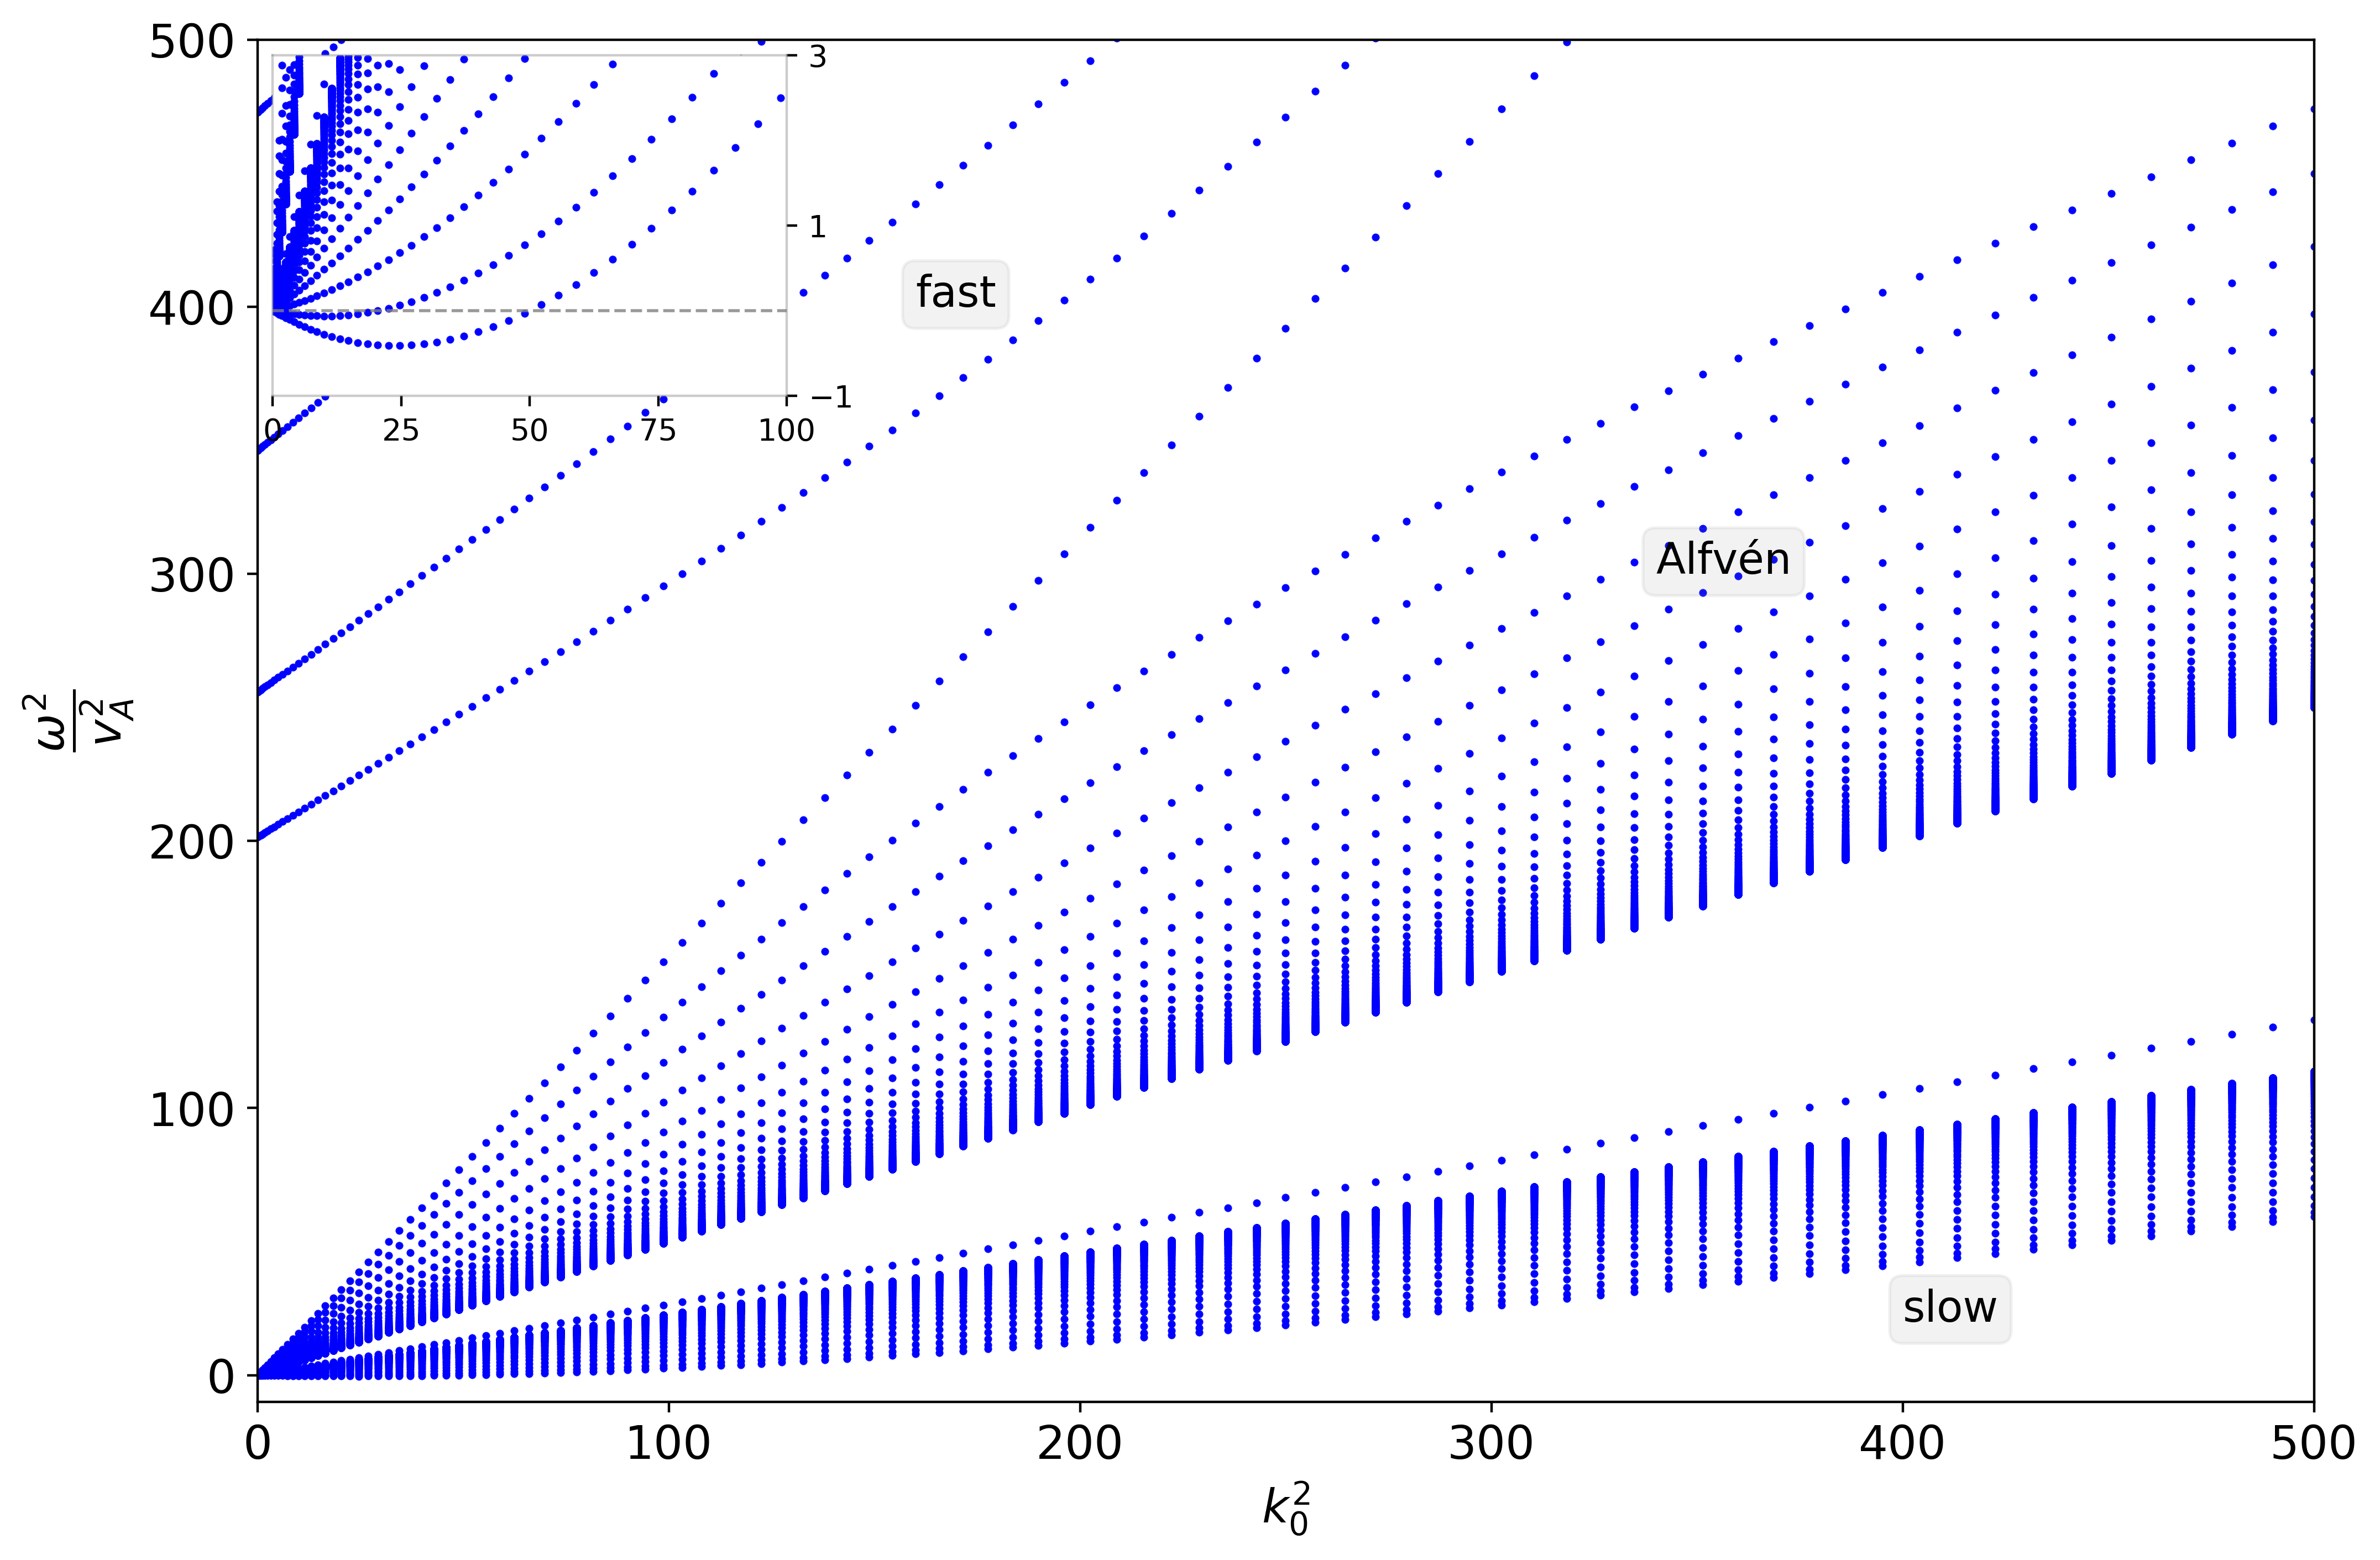
\includegraphics[width=\textwidth]{gravito_mhd.png}
  \caption{
    Spectrum of gravito-MHD modes, obtained through 100 {\legolas} runs of 351 gridpoints each. The fast (top), Alfv\'en (middle) and slow (bottom) branches of the MHD spectrum are clearly visible. The inset shows unstable slow modes at low frequencies.
  }
  \label{fig: gravito_mhd}
\end{figure}

The results are shown in Figure \ref{fig: gravito_mhd}, where every vertical collection of points at the same $k_0^2$ value represents one single {\legolas} run. Because we are in an MHD regime with a plasma $\beta = 1$, the three MHD subspectra can be clearly distinguished, showing the fast $p$ modes (top-left branches), Alfv\'en $g$ modes (middle branches), and slow $g$ modes (bottom branches). The inset shows a zoom-in near the marginal frequency of the spectrum, showing unstable $(\omega^2 < 0)$ slow MHD modes. These long-wavelength unstable modes are related to the Parker instabilities, due to magnetic buoyancy, as we will show in Section \ref{ss: quasi-parker}. Note that because this case is adiabatic and fully self-adjoint, every individual MHD spectrum is left-right and up-down symmetric in the complex eigenfrequency plane, but this aspect is hidden from the $\omega^2$ -- $k_0^2$ view shown here.


\subsection{Quasi-Parker instabilities} \label{ss: quasi-parker}
Next we discuss a modified case of the gravito-MHD waves, namely a spectrum showing quasi-Parker instabilities as done in \citet[Figure 12.2]{book_MHD}. The difference with the previous case is that a fully analytic description is no longer possible, because the introduction of magnetic shear leads to continuous ranges in the MHD spectrum. Instead of showing the spectrum for one single value for $\theta$, we now vary the direction of the wave vector $\bk_0$ between 0 and $\pi$. The equilibrium configuration is similar to the one in Section \ref{ss: gravito-mhd}, given in Cartesian geometry by
\begin{equation} \label{eq: quasi-parker}
  \begin{gathered}
    \rho_0 = \rho_c \exp\left(-\alpha x\right),
    \qquad
    p_0 = p_c \exp\left(-\alpha x\right),
    \qquad
    \alpha = \frac{\rho_c g}{p_c + \frac{1}{2}B_c}, \\
    B_{02} = B_c \exp\left(-\frac{1}{2}\right)\sin\left(\lambda x\right),
    \qquad
    B_{03} = B_c \exp\left(-\frac{1}{2}\right)\cos\left(\lambda x\right),
  \end{gathered}
\end{equation}
where magnetic shear was introduced through the parameter $\lambda$. The quantities $\alpha$ and $B_c$ are assigned the same values as in Equation \eqref{eq: gravito_mhd}; though now $g = 0.5$ and $p_c = 0.25$, which yield a plasma beta $\beta = 0.5$. The wave vectors are given by $k_y = \pi\sin(\theta)$ and $k_z = \pi\cos(\theta)$, such that $k_0^2 \approx 10$. The angle $\theta$ was varied between 0 and $\pi$ for a total of 100 runs at 351 grid points each, shown in Figure \ref{fig: quasi_parker}.

The left panels handle the case without magnetic shear, that is, $\lambda = 0$, which basically reduces to the one from the previous subsection. In this case, the slow and Alfv\'en continua collapse into single point values, denoted in red and cyan, respectively. The right panels show the same configuration where $\lambda = 0.3$ was taken, introducing magnetic shear, which introduces genuine continua seen as bands. These continua affect the overall stability and organise the entire MHD spectrum: all discrete modes are fully aware of the essential spectrum formed by these (slow and Alfv\'en) continua and the (fast) accumulation points at infinite frequency. All features of the original figure in \citet{book_MHD} are reproduced. The inset zooms into the region where both continua overlap, showing quasi-interchange and interchange instabilities. Once more, each run, shown here collectively in Figure \ref{fig: quasi_parker}, actually has a spectrum that is left-right and up-down symmetric in the eigenfrequency plane. This is depicted on Panels c and d, which show the eigenfrequency view for one single case $(\theta = 0.3\pi)$. The continuum ranges separate nicely: the collapsed single point values are denoted by cyan (Alfv\'en) and red (slow) points on Panel c, and the genuine continua are shown with cyan and red bands on Panel d. The instabilities themselves are situated on the (positive) imaginary axis, due to the self-adjointness of the eigenvalue problem.

\begin{figure}[t]
  \centering
  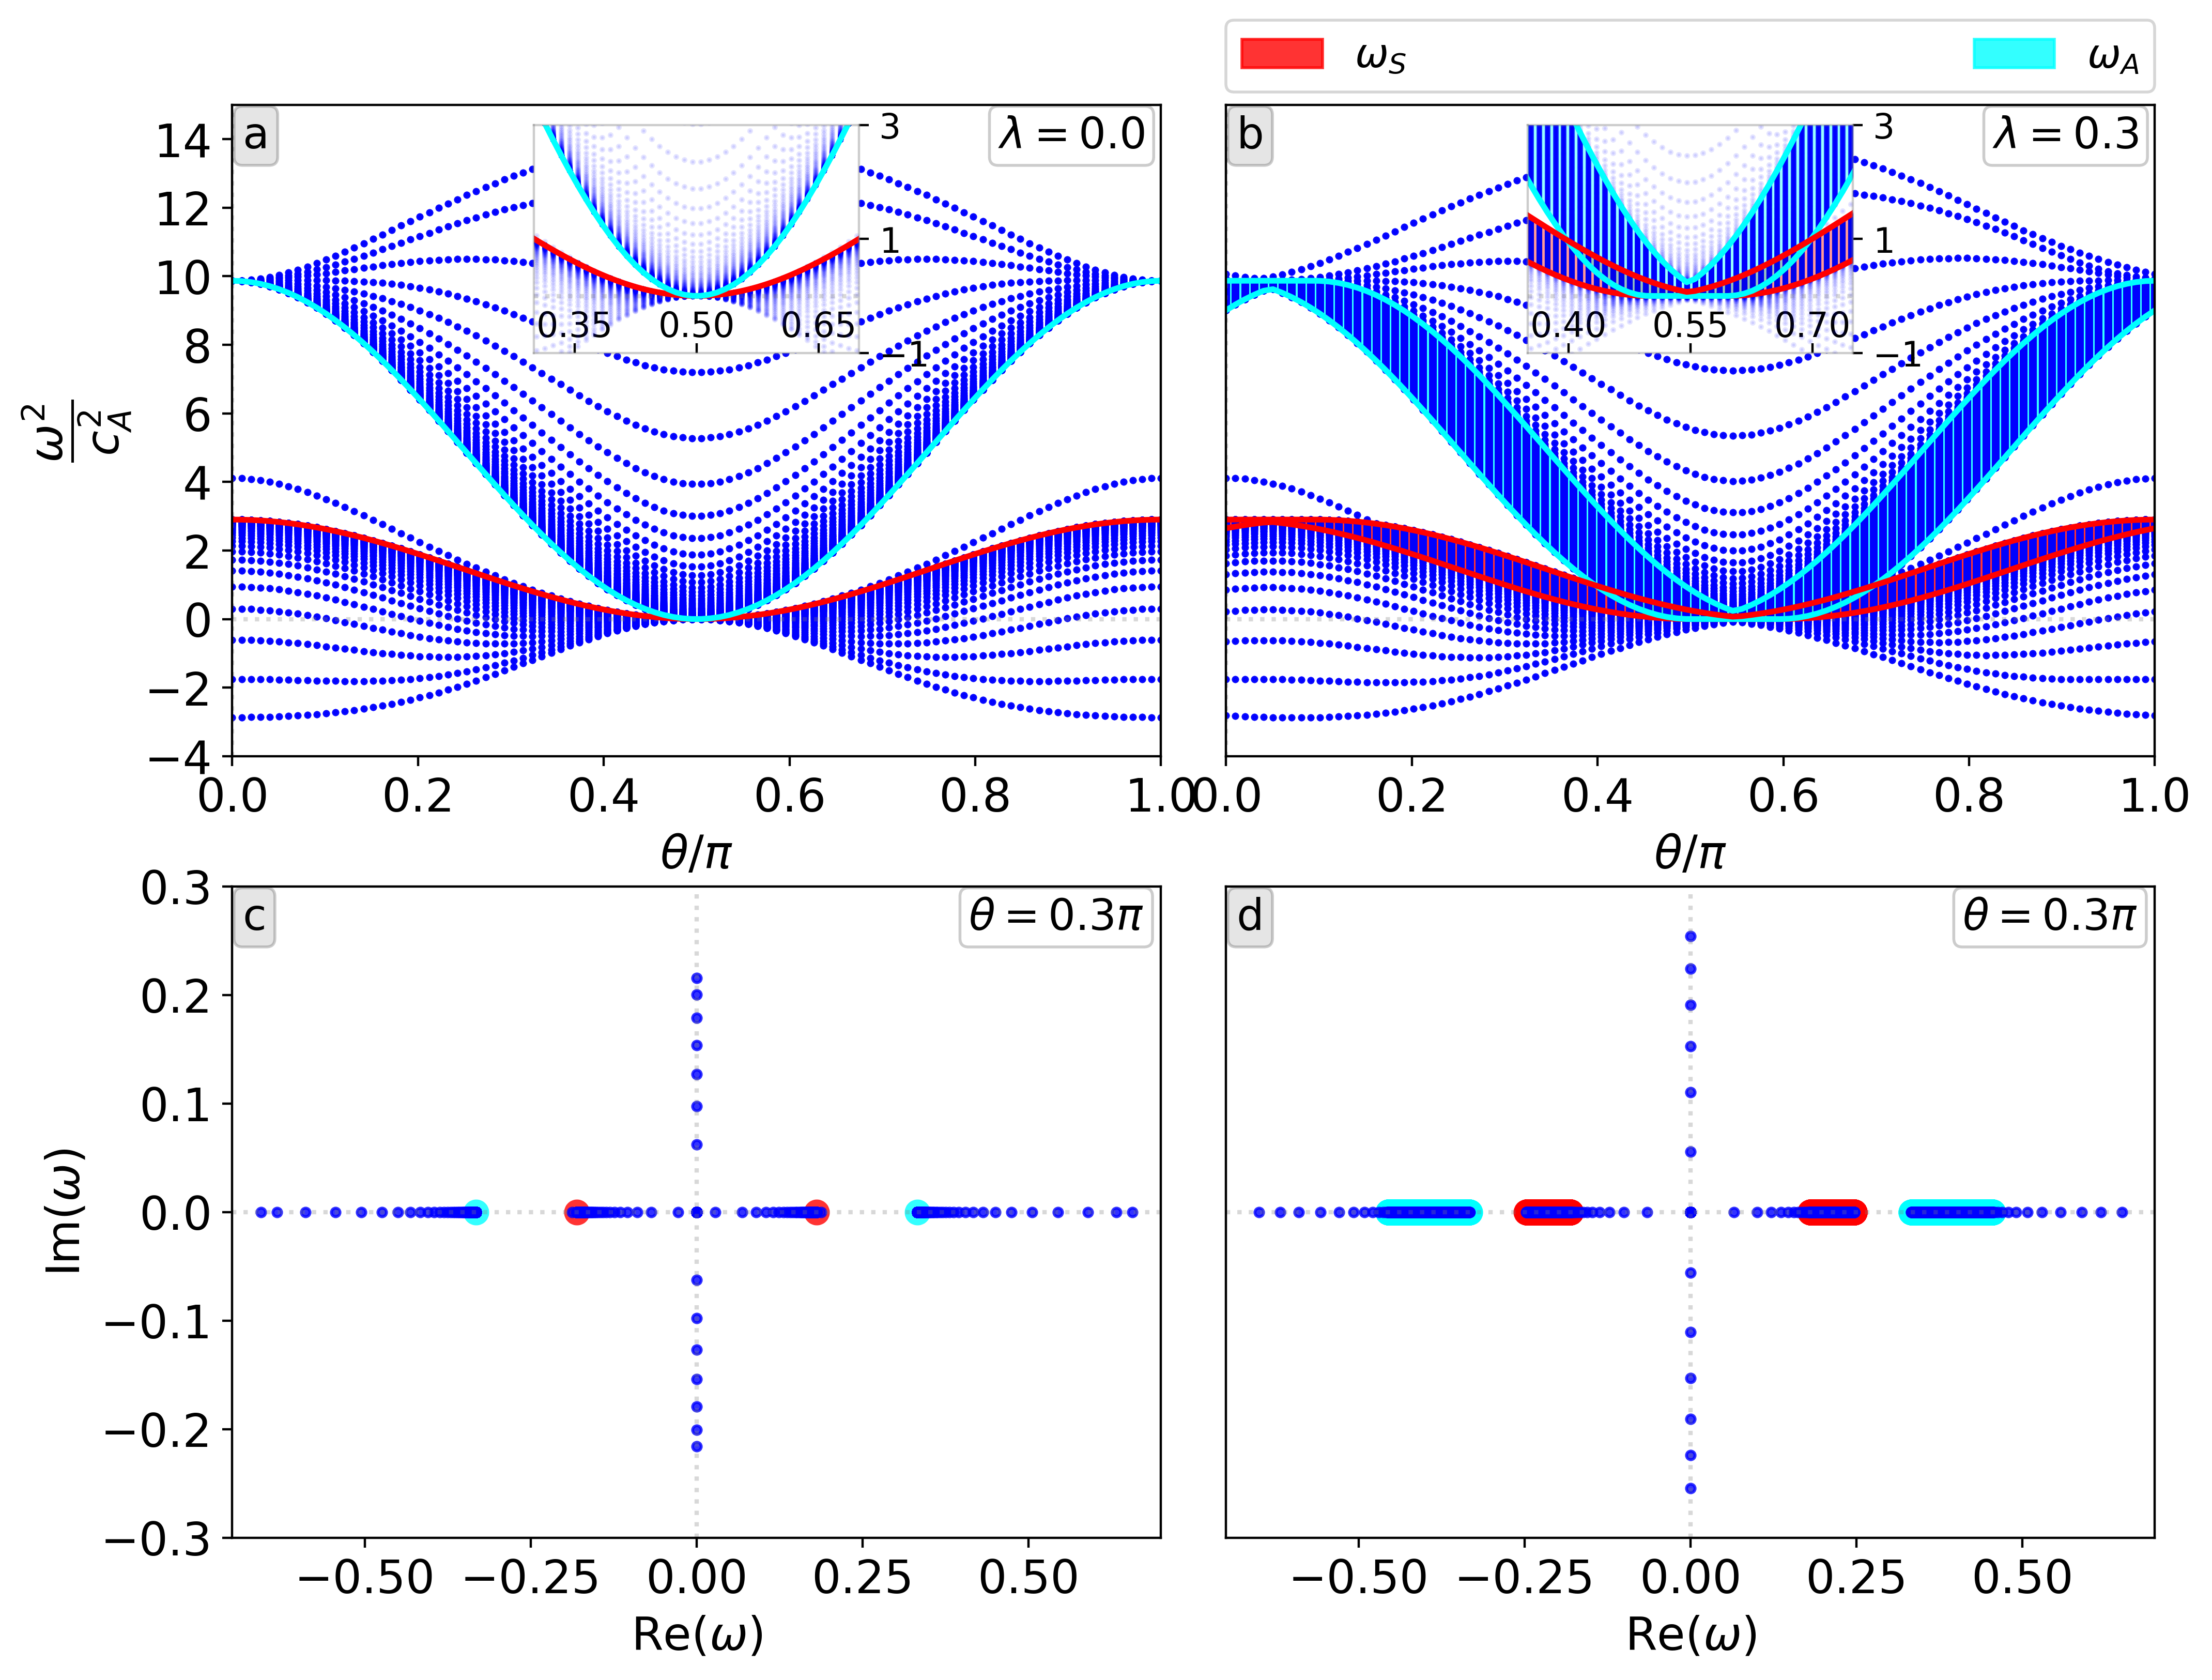
\includegraphics[width=\textwidth]{quasi_parker.png}
  \caption{
    Spectrum showing Parker and quasi-Parker modes without (\textbf{a}, \textbf{c}) and with (\textbf{b}, \textbf{d}) magnetic shear. The slow and Alfv\'en continua are shown in red and cyan, respectively, where the insets zoom into the region of quasi-interchange modes. The bottom row of panels show the eigenfrequency view for the single case $\theta = 0.3\pi$. The continua are again annotated in the panels, visualising the collapsed single point values (Panel \textbf{c}) as well as the genuine continuum ranges (Panel \textbf{d}).
  }
  \label{fig: quasi_parker}
\end{figure}

As explained in \citet{book_MHD}, we see from this eigenmode computation that the Parker instability, which is there for $\bk_0$ parallel to $\bb_0$, becomes a quasi-Parker instability away from perfect alignment and connects smoothly to well-known quasi-interchange instabilities that occur here (marginally) away from perpendicular orientation. Quantifying how the equilibrium parameters influence the growth rates of these unstable branches can only be done numerically, for example with {\legolas}.

\section{Adiabatic, cylindrical cases}
Next we move on to cylindrical configurations, which provide tests for the scale factor $\eps$ in the equations. Analytical results from the literature are again well reproduced. Furthermore, we look at different spectra previously obtained by the LEDA code, discussed in various papers, and compare those with the new spectra from {\legolas}.

\subsection{Magnetic flux tubes}
The first case that we describe in this subsection is a magnetic flux tube embedded in a uniform magnetic environment, discussed in \citet{book_roberts}. The equilibrium configuration is simple, in the sense that we have a uniform magnetic field aligned with the $z$-axis both inside and outside of the flux tube, with a similar structure for the other equilibrium parameters:
\begin{equation}
  B_0(r), \rho_0(r), p_0(r), T_0(r) =
  \begin{cases}
    B_0, \rho_0, p_0, T_0, \qquad &r < a \\
    B_\text{e}, \rho_\text{e}, p_\text{e}, T_\text{e}, \qquad &r > a
  \end{cases}
\end{equation}
where the subscripts ``0'' and ``e'' refer to values inside the tube and for the environment, respectively. The outer radius of the tube is denoted by $a$ and hence represents a discontinuous interface between the tube itself and the environment. Because total pressure balance should be preserved across the boundary, which is something that follows from Equation \eqref{eq: force_equilibrium}, this yields a relation between pressures and magnetic field components inside and outside of the tube, which in turn implies a connection between the plasma densities, sound speeds, and Alfv\'en speeds across the boundary:
\begin{equation} \label{eq: flux_tube_pbalance}
  p_0 + \frac{1}{2}B_0^2 = p_\text{e} + \frac{1}{2}B_\text{e}^2, \qquad\qquad
  \frac{\rho_e}{\rho_0} = \frac{\soundspeed^2 + \dfrac{1}{2}\gamma \alfvenspeed^2}{
    c_\text{se}^2 + \dfrac{1}{2}\gamma c_\text{Ae}^2},
\end{equation}
where $\soundspeed^2 = \gamma p_0 / \rho_0$ and $\alfvenspeed^2 = B_0^2 / \rho_0$ denote the sound speed and Alfv\'en speed, respectively, in which the values outside of the flux tube are used if there is a subscript e present.

It should be noted that this extremely simple equilibrium configuration is the standard case used in many solar coronal loop seismology efforts. Because it simply has two uniform media (one inside the tube and one in its exterior), it has no continuous spectra (they reduce to point values), but the interface makes it possible to again have surface modes that would be affected by true radial variation. Also note that these flux tubes have only stable waves, but we can distinguish between body and surface waves, depending on the variation of the eigenfunctions within the flux tube. In the exterior of the flux tube all eigenfunctions are exponentially varying.

We should also clarify here that the original dispersion relation as given in \citet{book_roberts} assumes a flux tube embedded in an environment extending towards infinity, while {\legolas} on the other hand assumes a fixed wall boundary at the outer edge of the domain. Hence, we assume here that the domain is situated in $r \in [0, 10]$ with the inner flux tube wall at $r = 1$ in order to minimise the outer wall influence. However, this introduces an additional computational challenge, in the sense that we are (mainly) interested in the behaviour of the inner modes, because we know that the outer modes all have exponentially varying eigenfunctions which decay to infinity (or toward our far-away outer wall). Hence, in order to resolve those inner waves huge resolutions are needed due to the $1:10$ radio. In order to circumvent this issue we used a simple prescription for mesh refinement, that is, a 60--30--10 division of the initial nodes. This means that $60\%$ of the grid points are used for the inner tube region $r \in [0, 0.95]$, $30\%$ of the grid points are located near the transition region $r \in [0.95, 1.05]$, and the remaining $10\%$ are used for the environment $r \in [1.05, 10]$.

\paragraph{(a) Photospheric flux tube.}
First, we look at a flux tube under photospheric conditions, that is, an equilibrium for which $c_\text{Ae} < \soundspeed < c_\text{se} < \alfvenspeed$. More specifically, we take $c_\text{Ae} = \soundspeed/2$, $c_\text{se} = 3\soundspeed / 2$, and $\alfvenspeed = 2\soundspeed$ following \citet[Figure 6.5]{book_roberts}. The relations between the inner and outer regions of the flux tube follow straightforwardly from Equation \eqref{eq: flux_tube_pbalance}, and hence we only have two degrees of freedom, namely $\rho_0$ and $p_0$, which are both taken to unity, with $\gamma = 5/3$. This results in $\rho_0 \approx 0.567~\rho_\text{e}$, $\tubespeed \approx 0.89~\soundspeed$,
$\kinkspeed \approx 0.63~\alfvenspeed \approx 1.27~\soundspeed$. Here we also introduced the tube and kink speeds, given by
\begin{equation}
  \tubespeed^2 = \frac{\soundspeed^2 \alfvenspeed^2}{\soundspeed^2 + \alfvenspeed^2}, \qquad\qquad
  \kinkspeed^2 = \frac{\rho_0 \alfvenspeed^2 + \rho_\text{e}c_\text{Ae}^2}{\rho_0 + \rho_\text{e}},
\end{equation}
using the same notation as in Equation \eqref{eq: flux_tube_pbalance}. As described before, we take $r \in [0, 10]$ and place the flux tube boundary at $a = 1$. Next we perform 40 runs at 300 gridpoints each for four azimuthal wavenumbers $m = 0$ to $m = 3$. For the wavenumber $k_3 = k_z$, we take 40 values in such a way that the dimensionless wavenumber $k_z a$ has values in $[0, 6.2]$. The spectrum showing the dispersion relation, where the dimensionless phase speed $\omega / k_z \soundspeed$ is plotted as a function of $k_z a$, is depicted in Figure \ref{fig: fluxtube_coronal}.

\begin{figure}[t]
  \centering
  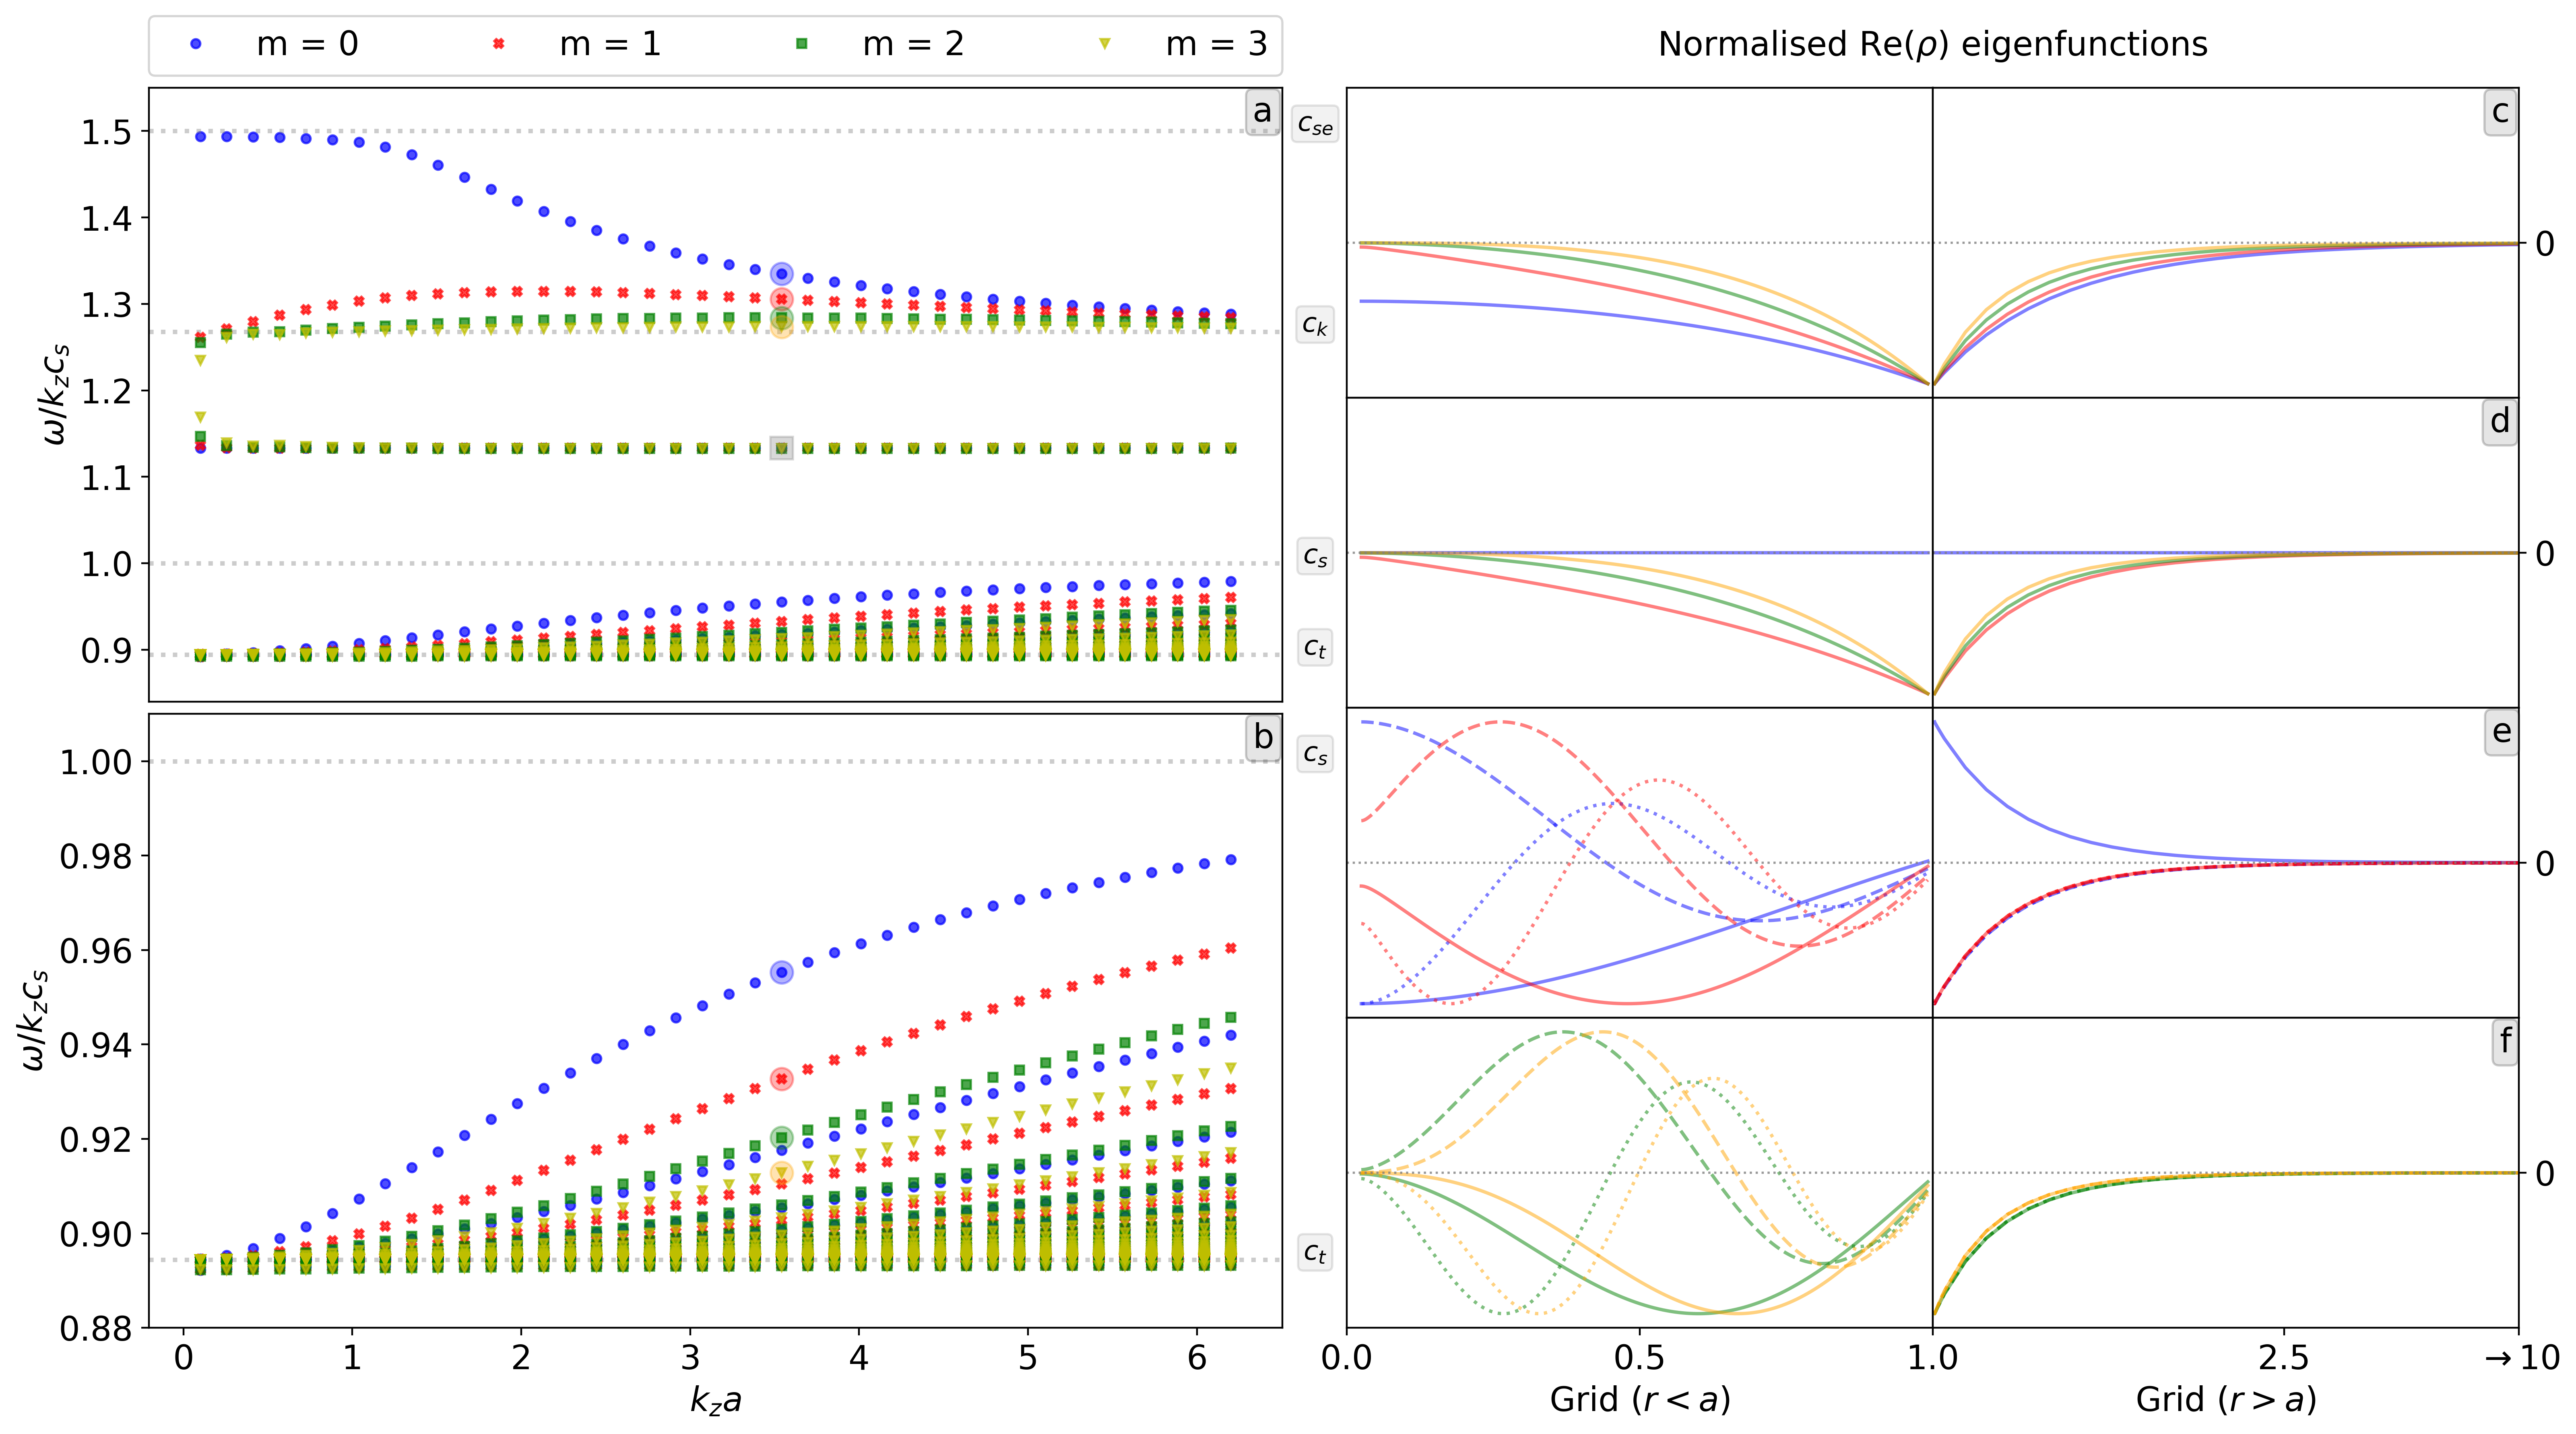
\includegraphics[width=\textwidth]{fluxtube_photospheric.png}
  \caption{
    Panel \textbf{a}: spectrum showing the dispersion relation for a flux tube under photospheric conditions. The dimensionless phase speed $\omega / k_z \soundspeed$ is displayed as a function of the dimensionless wavenumber $k_z a$ for four values of the azimuthal wavenumber $m = 0$ (blue dots), $m = 1$ (red crosses), $m = 2$ (green squares), and $m = 3$ (yellow triangles). Both sound speeds, the kink speed, and the tube speed are denoted using dashed grey horizontal lines, all normalised to $\soundspeed$. Panel \textbf{b}: zoom-in of Panel \textbf{a} between the tube speed $\tubespeed$ and internal sound speed $\soundspeed$. Panels \textbf{c} and \textbf{d}: eigenfunctions of the modes associated with circles (\textbf{c}) and squares (\textbf{d}) on the top-left Panel \textbf{a}. Panel \textbf{e}: first three eigenfunctions of the $m = 0$ and $m = 1$ body wave sequence on Panel \textbf{b}. Panel \textbf{f}: first three eigenfunctions of the $m = 2$ and $m = 3$ body wave sequence. For both panels \textbf{e} and \textbf{f}, the $n = 1$, $n = 2$, and $n = 3$ modes are shown in solid, dashed and dotted lines, respectively; only the first mode is annotated on the bottom-left Panel. Every eigenfunction in panels \textbf{c}--\textbf{f} is normalised to its maximum absolute value in that particular grid interval.
  }
  \label{fig: fluxtube_photospheric}
\end{figure}

All speeds indicated in the figure are normalised to the internal sound speed $\soundspeed$. Panel a clearly shows the fast surface waves, including the sausage $(m = 0)$, kink $(m = 1)$, and first two fluting modes ($m = 2$ and $m = 3$). The eigenfunctions in Panel c correspond to the modes annotated with a transparent circle in Panel a, with colours indicating the mode number $m$. The left and right sides of Panels c--f show the eigenfunctions for the inner and outer regions of the flux tube, respectively. All eigenfunctions are normalised to their maximum value, and all eigenvalues having a normalised phase speed larger than 1.5 are not shown. It should be noted that the first three runs, that is, the first three dots according to the $k_z a$ axis, were done using 1001 gridpoints. The reason for this is that when we divide the eigenvalues $\omega$ by $k_z$, small errors are increased selectively for small $k_z$, explaining why those modes seem slightly scattered and hence why he have to employ such high resolutions in order to minimise said error.

Panel b of Figure \ref{fig: fluxtube_photospheric} zooms in between the tube speed ($\tubespeed$) and internal sound speed ($\soundspeed$), showing a clear representation of the various body waves that accumulate to the tube speed at long wavelengths. Panel e shows the first three modes of the $m = 0$ and $m = 1$ sequences in solid, dashed, and dotted lines, respectively; that is, the first mode in the sequence (solid line) corresponds to the mode annotated in Panel b. The next two modes in that sequence are the next two blue dots moving vertically downwards (same $k_z a$ value), these are not annotated to avoid cluttering the figure. Analogously, Panel f shows the first three modes of the $m = 2$ and $m = 3$ sequences, with everything colour-coded according to the legend. As indicated before, all eigenfunctions in the outer region are exponentially varying. Panels a and b in Figure \ref{fig: fluxtube_photospheric} reproduce the analytical results in \citet[Figure 6.5]{book_roberts}.

One mode has not yet been discussed, and that is the horizontal line of modes between the internal sound speed and kink speed. The eigenfunctions are shown in Panel d and correspond to the annotated squares in the top-left Panel a. These modes are not present in the original work, and it is not a priori clear how to interpret them. These modes are degenerate, meaning that their position does not change when the mode number $m$ or wavenumber $k_z$ changes. The position of the outer wall also does not seem to have any influence on their value, and their eigenfunctions seem to indicate that these are surface waves. However, it is also quite possible that these modes are a numerical remnant of the discontinuous equilibrium profile, and are picked up by {\legolas} due to the sharp transition between the inner flux tube and the environment at $a = 1$.

\paragraph{(b) Coronal flux tube.} The second application of the magnetic flux tube is one under coronal conditions, that is, an equilibrium for which $c_\text{se} < \soundspeed < \alfvenspeed < c_\text{Ae}$. More specifically, we take
$c_\text{Ae} = 5\soundspeed$, $c_\text{se} = \soundspeed/2$, and $\alfvenspeed = 2\soundspeed$. Analogous to the previous case, the relations between the equilibrium values inside and outside of the flux tube follow from Equation \eqref{eq: flux_tube_pbalance}, where we again take $p_0$ and $\rho_0$ to be equal to one. This results in
$\rho_0 \approx 4.86~\rho_\text{e}$, $\tubespeed \approx 0.89~\soundspeed$, and
$\kinkspeed \approx 1.38~\alfvenspeed \approx 0.55~c_\text{Ae}$, and we use the same values as for the photospheric case for $k_z$ and the flux tube and outer wall boundaries. Similar to case (a), we perform 40 runs at 300 gridpoints each for four values of $k_2 = m$ (where again the first three runs have 1001 gridpoints) and plot the spectrum showing the dispersion relation in Figure \ref{fig: fluxtube_coronal}. Again, all speeds indicated in the figure are normalised to the sound speed $\soundspeed$. The top-left Panel a focuses on the fast body waves, the bottom-left Panel b on the slow body waves. Panel c shows the eigenfunctions corresponding to the four body waves indicated with circles in Panel a. Panel d depicts the eigenfunctions of the modes annotated with squares between the internal Alfv\'en ($\alfvenspeed$) and kink ($\kinkspeed$) speeds, representing the kink $m = 1$ and first two fluting ($m = 2$ and $m = 3$) modes.

\begin{figure}[t]
  \centering
  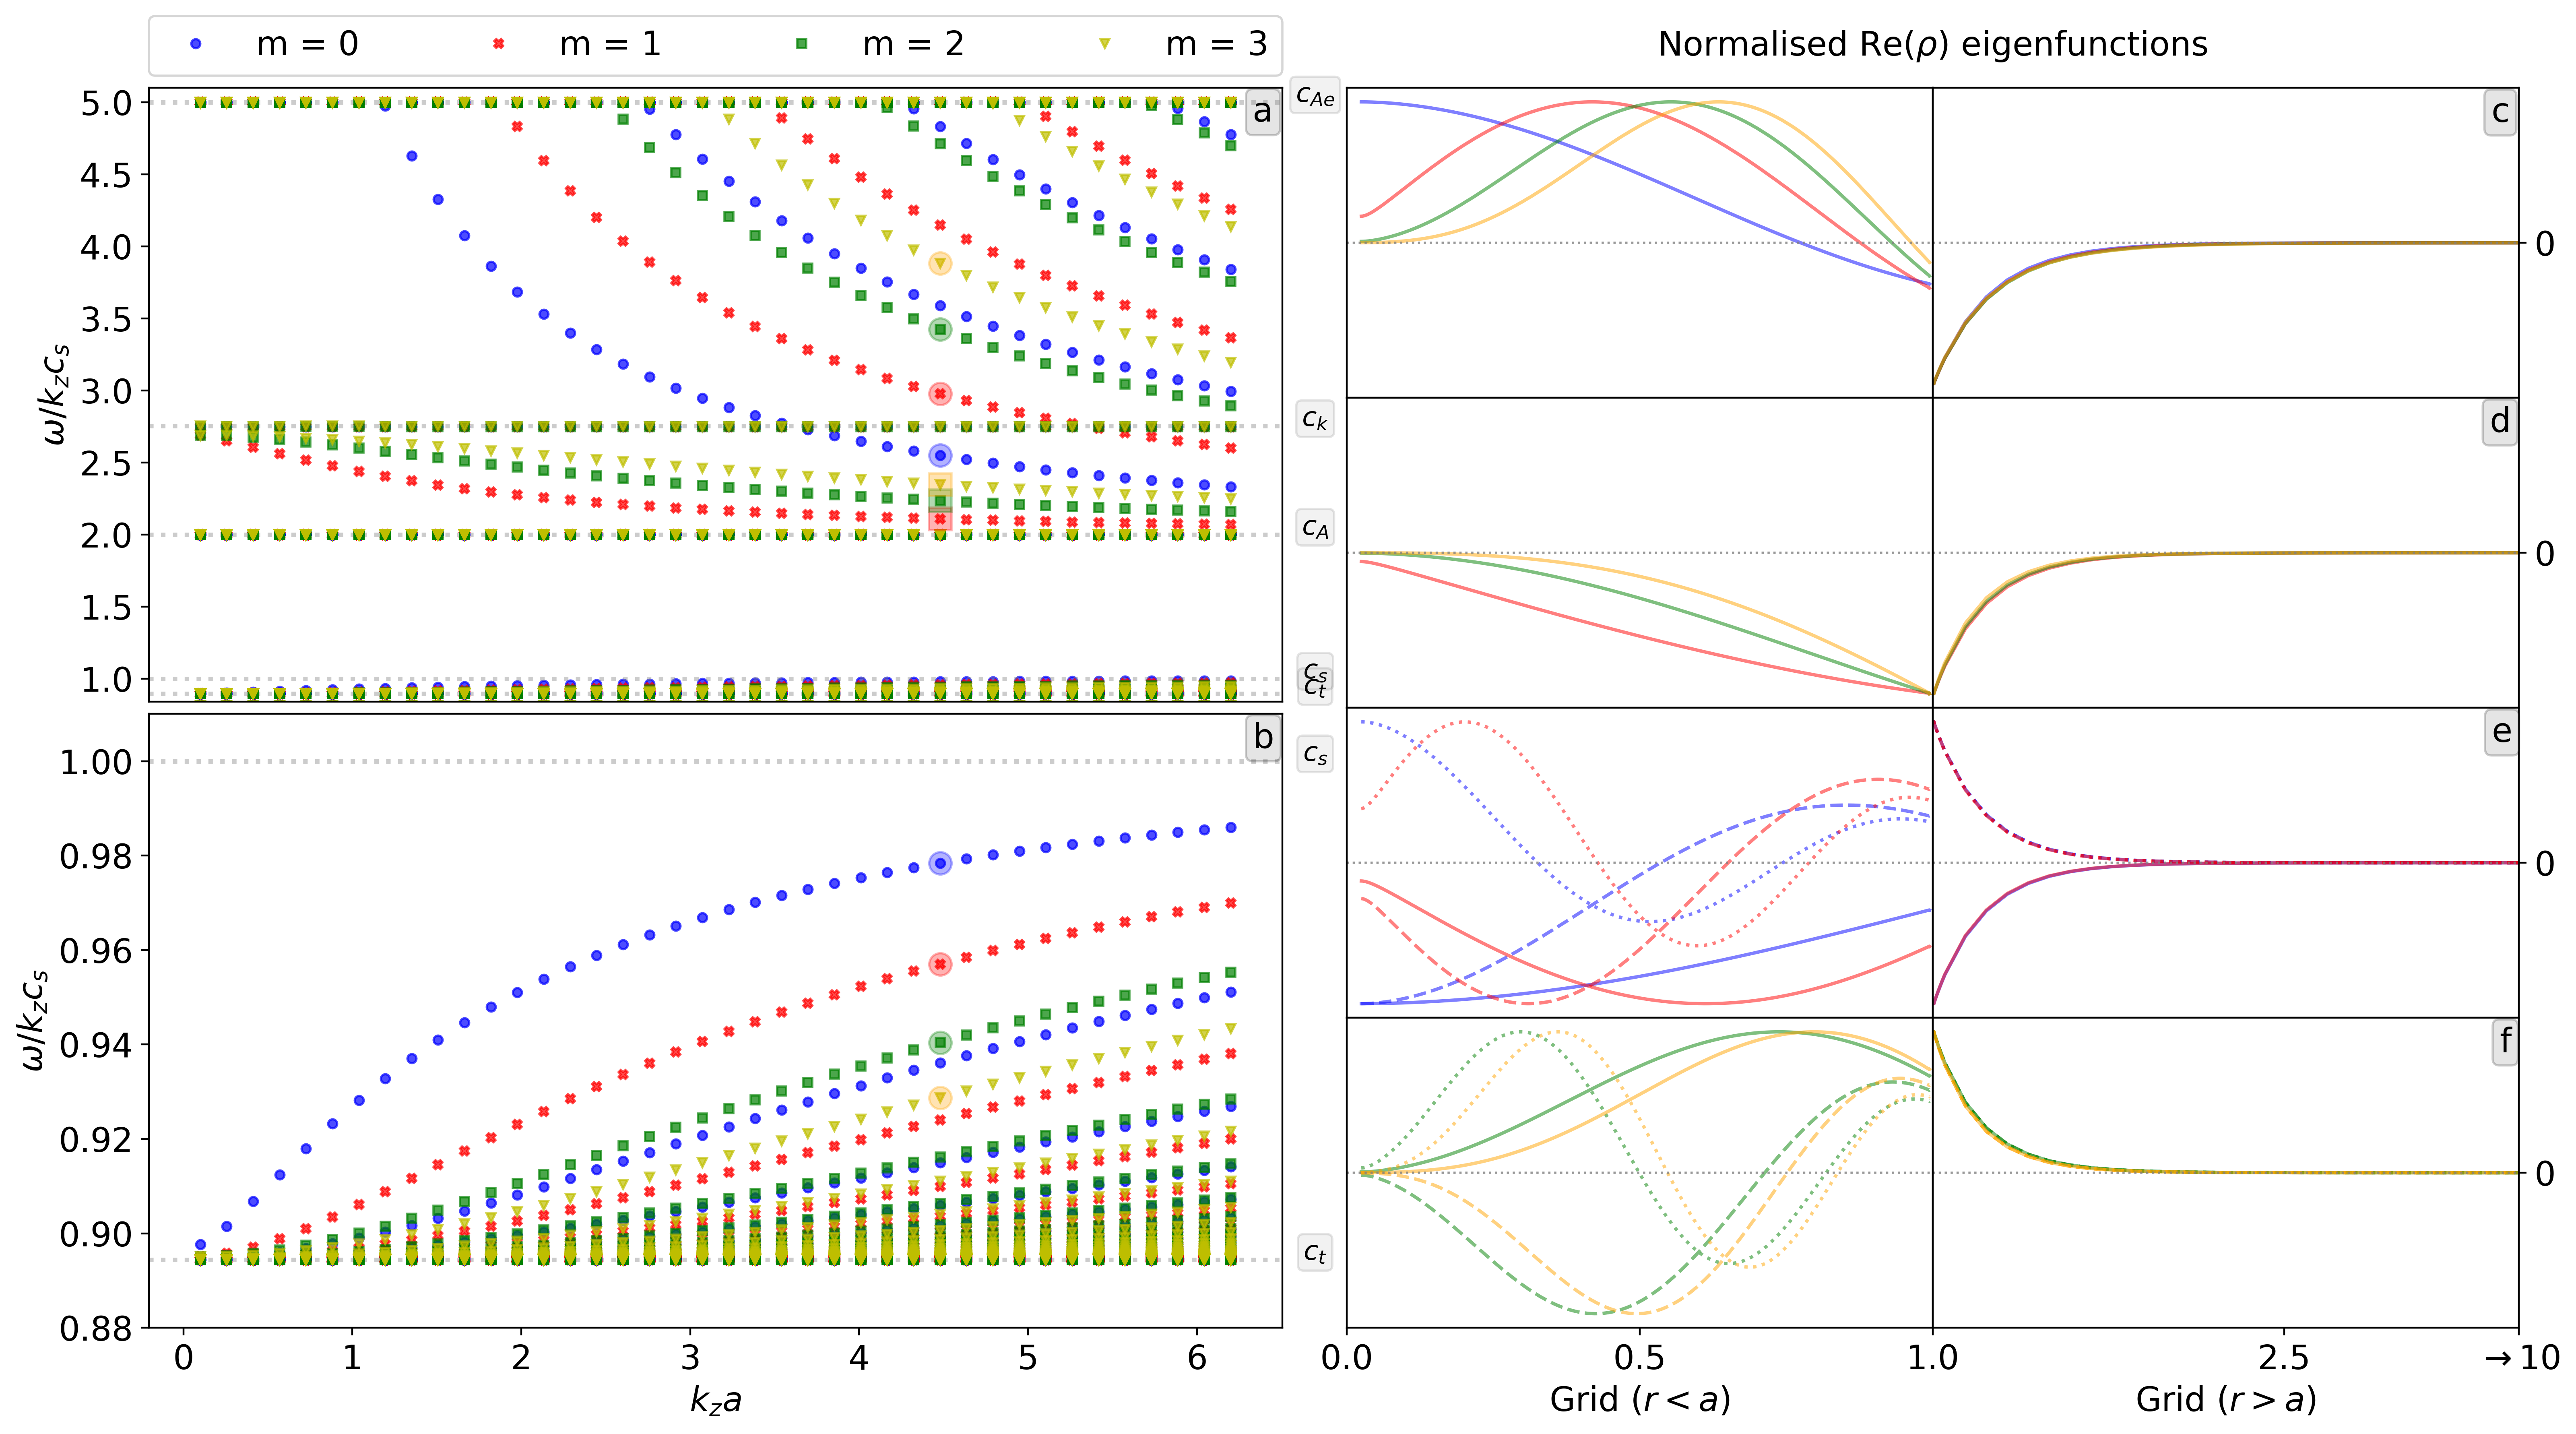
\includegraphics[width=\textwidth]{fluxtube_coronal.png}
  \caption{
    Panel \textbf{a}: spectrum showing the dispersion relation for a flux tube under coronal conditions. The dimensionless phase speed $\omega / k_z \soundspeed$ is displayed as a function of the dimensionless wavenumber $k_z a$ for four values of the azimuthal wavenumber $m = 0$ (blue dots), $m = 1$ (red crosses), and $m = 2$ (green squares), and $m = 3$ (yellow triangles). Both Alfv\'en speeds, together with the kink, tube, and sound speeds are denoted by grey horizontal lines and are all normalised to $\soundspeed$. Panel \textbf{b} zoom-in of Panel \textbf{a} between the tube speed $\tubespeed$ and internal sound speed $\soundspeed$, zooming in on the tube-speed-related body mode sequences. Panels \textbf{c} and \textbf{d}: eigenfunctions of the modes annotated with circles (\textbf{c}) and squares (\textbf{d}) on the top-left Panel \textbf{a}. Panel \textbf{e}: first three eigenfunctions of the $m = 0$ and $m = 1$ body wave sequence in the bottom-left Panel \textbf{b}. Panel \textbf{f}: first three eigenfunctions of the $m = 2$ and $m = 3$ body wave sequence. For both Panels \textbf{e} and \textbf{f} the $n = 1$, $n = 2$ and $n = 3$ modes are shown in solid, dashed and dotted lines, respectively, only the first mode is annotated on Panel \textbf{b}. Every eigenfunction in Panels \textbf{c}--\textbf{f} is normalised to its maximum absolute value in that particular grid interval.
  }
  \label{fig: fluxtube_coronal}
\end{figure}

Similar to Figure \ref{fig: fluxtube_photospheric}, Panels e and f represent the first three body modes in the $m = 0$ and $m = 1$ sequences (Panel e), of which the first mode is indicated in Panel b. Panel f shows the first three modes of the $m = 2$ and $m = 3$ sequences, with the first, second, and third modes indicated with a solid, dashed and dotted line, respectively. The colours of Panels c--f are consistent with the legend. Figure \ref{fig: fluxtube_coronal} reproduces the analytical results in \citet[Figure 6.7]{book_roberts}, which are based on the analytic dispersion relation containing Bessel functions.

\subsection{Tokamak current profile}
Next we discuss an example initially given in \citet{kerner1985}, which shows the ideal MHD spectrum in the presence of an unstable $m = -2$ interchange mode in a cylindrical geometry. We start from a so-called tokamak current profile, in which an axial current density of the form $\boldsymbol{j}_0 = \left(0, 0, j_0(1 - r^2)^\nu\right)$ is assumed, with $j_0$ a given constant. This yields a twisted magnetic field profile in which the longitudinal component $B_{0z}$ is uniform and equals one, while the poloidal component $B_{0\theta}$ is given by
\begin{equation} \label{eq: tokamak_btheta}
  B_{0\theta} = \frac{j_0}{2r\left(\nu + 1\right)}\left[1 - \left(1 - r^2\right)^{\nu + 1}\right],
\end{equation}
for a given value of $\nu$. For the equilibrium considered here, we take $\nu = 0$, making the current profile constant over the flux tube. This means that $B_{0\theta}$ has a linear profile in $r$ such that the magnetic field lines have a constant pitch and the current is distributed equally in the plasma. An expression for the pressure (and hence temperature) can be found by integrating the force-balance Equation \eqref{eq: force_equilibrium} and assuming that, for example, the pressure vanishes at the outer boundary, resulting in a parabolic pressure profile. Hence, for a cylindrical geometry in which $r \in [0, 1]$, this yields the following equilibrium configuration:
\begin{equation}
  \begin{gathered}
    \rho_0 = 1,
    \qquad
    p_0 = \frac{1}{4}j_0^2\left(1 - r^2\right),
    \qquad
    B_{02} = \frac{1}{2}j_0 r,
    \qquad
    B_{03} = 1,
  \end{gathered}
\end{equation}
where we assumed a uniform density. We introduce an additional parameter $q$, called the \emph{safety factor}, given by
\begin{equation}
  q(r) = \frac{rk_z B_{0z}}{B_{0\theta}} = \frac{2k_z}{j_0}.
\end{equation}

We performed 39 runs, varying the $q$ factor between 1.9 and 2.1 in order to probe the regime containing the unstable $m = -2$ interchange mode, which is associated with the vanishing of the factor $m + kq$, that is, the $\bk \cdot \bb$ product. This implicitly constrains the value for $j_0$, and we assigned $k_2 = m = -2$ and $k_3 = k = 0.2$ for all runs. It should be noted that this particular equilibrium configuration requires a relatively high resolution near $q = 2$ to correctly resolve the unstable modes; here we used 501 gridpoints for all runs. The complete spectrum is shown in Figure \ref{fig: tokamak_current}, where the squared eigenvalues are plotted as a function of the safety factor. The three main branches, that is, fast, Alfv\'en and slow, are denoted on the right side of the figure, as well as the region where the modes become unstable $(\omega^2 < 0)$. We see that in the region near the $m = -2$ interchange instabilities, the slow and Alfv\'en modes collapse to zero, which is due to the vanishing of the combination $\Fplus$ (see Equation \eqref{eq: F_G_operators} in Chapter \ref{ch: legolas}) in the ideal MHD equations \citep{book_MHD}. The slow and Alfv\'en continua are annotated in the figure in red and cyan, respectively. The Alfv\'en continuum is collapsed to a single point for this equilibrium configuration, while the slow continuum covers a range in frequency. Note in particular how the full spectrum ranges over many orders of magnitude in the $\omega^2$ view shown here: an intrinsic property (and challenge!) posed by MHD spectral theory.

\begin{figure}[t]
  \centering
  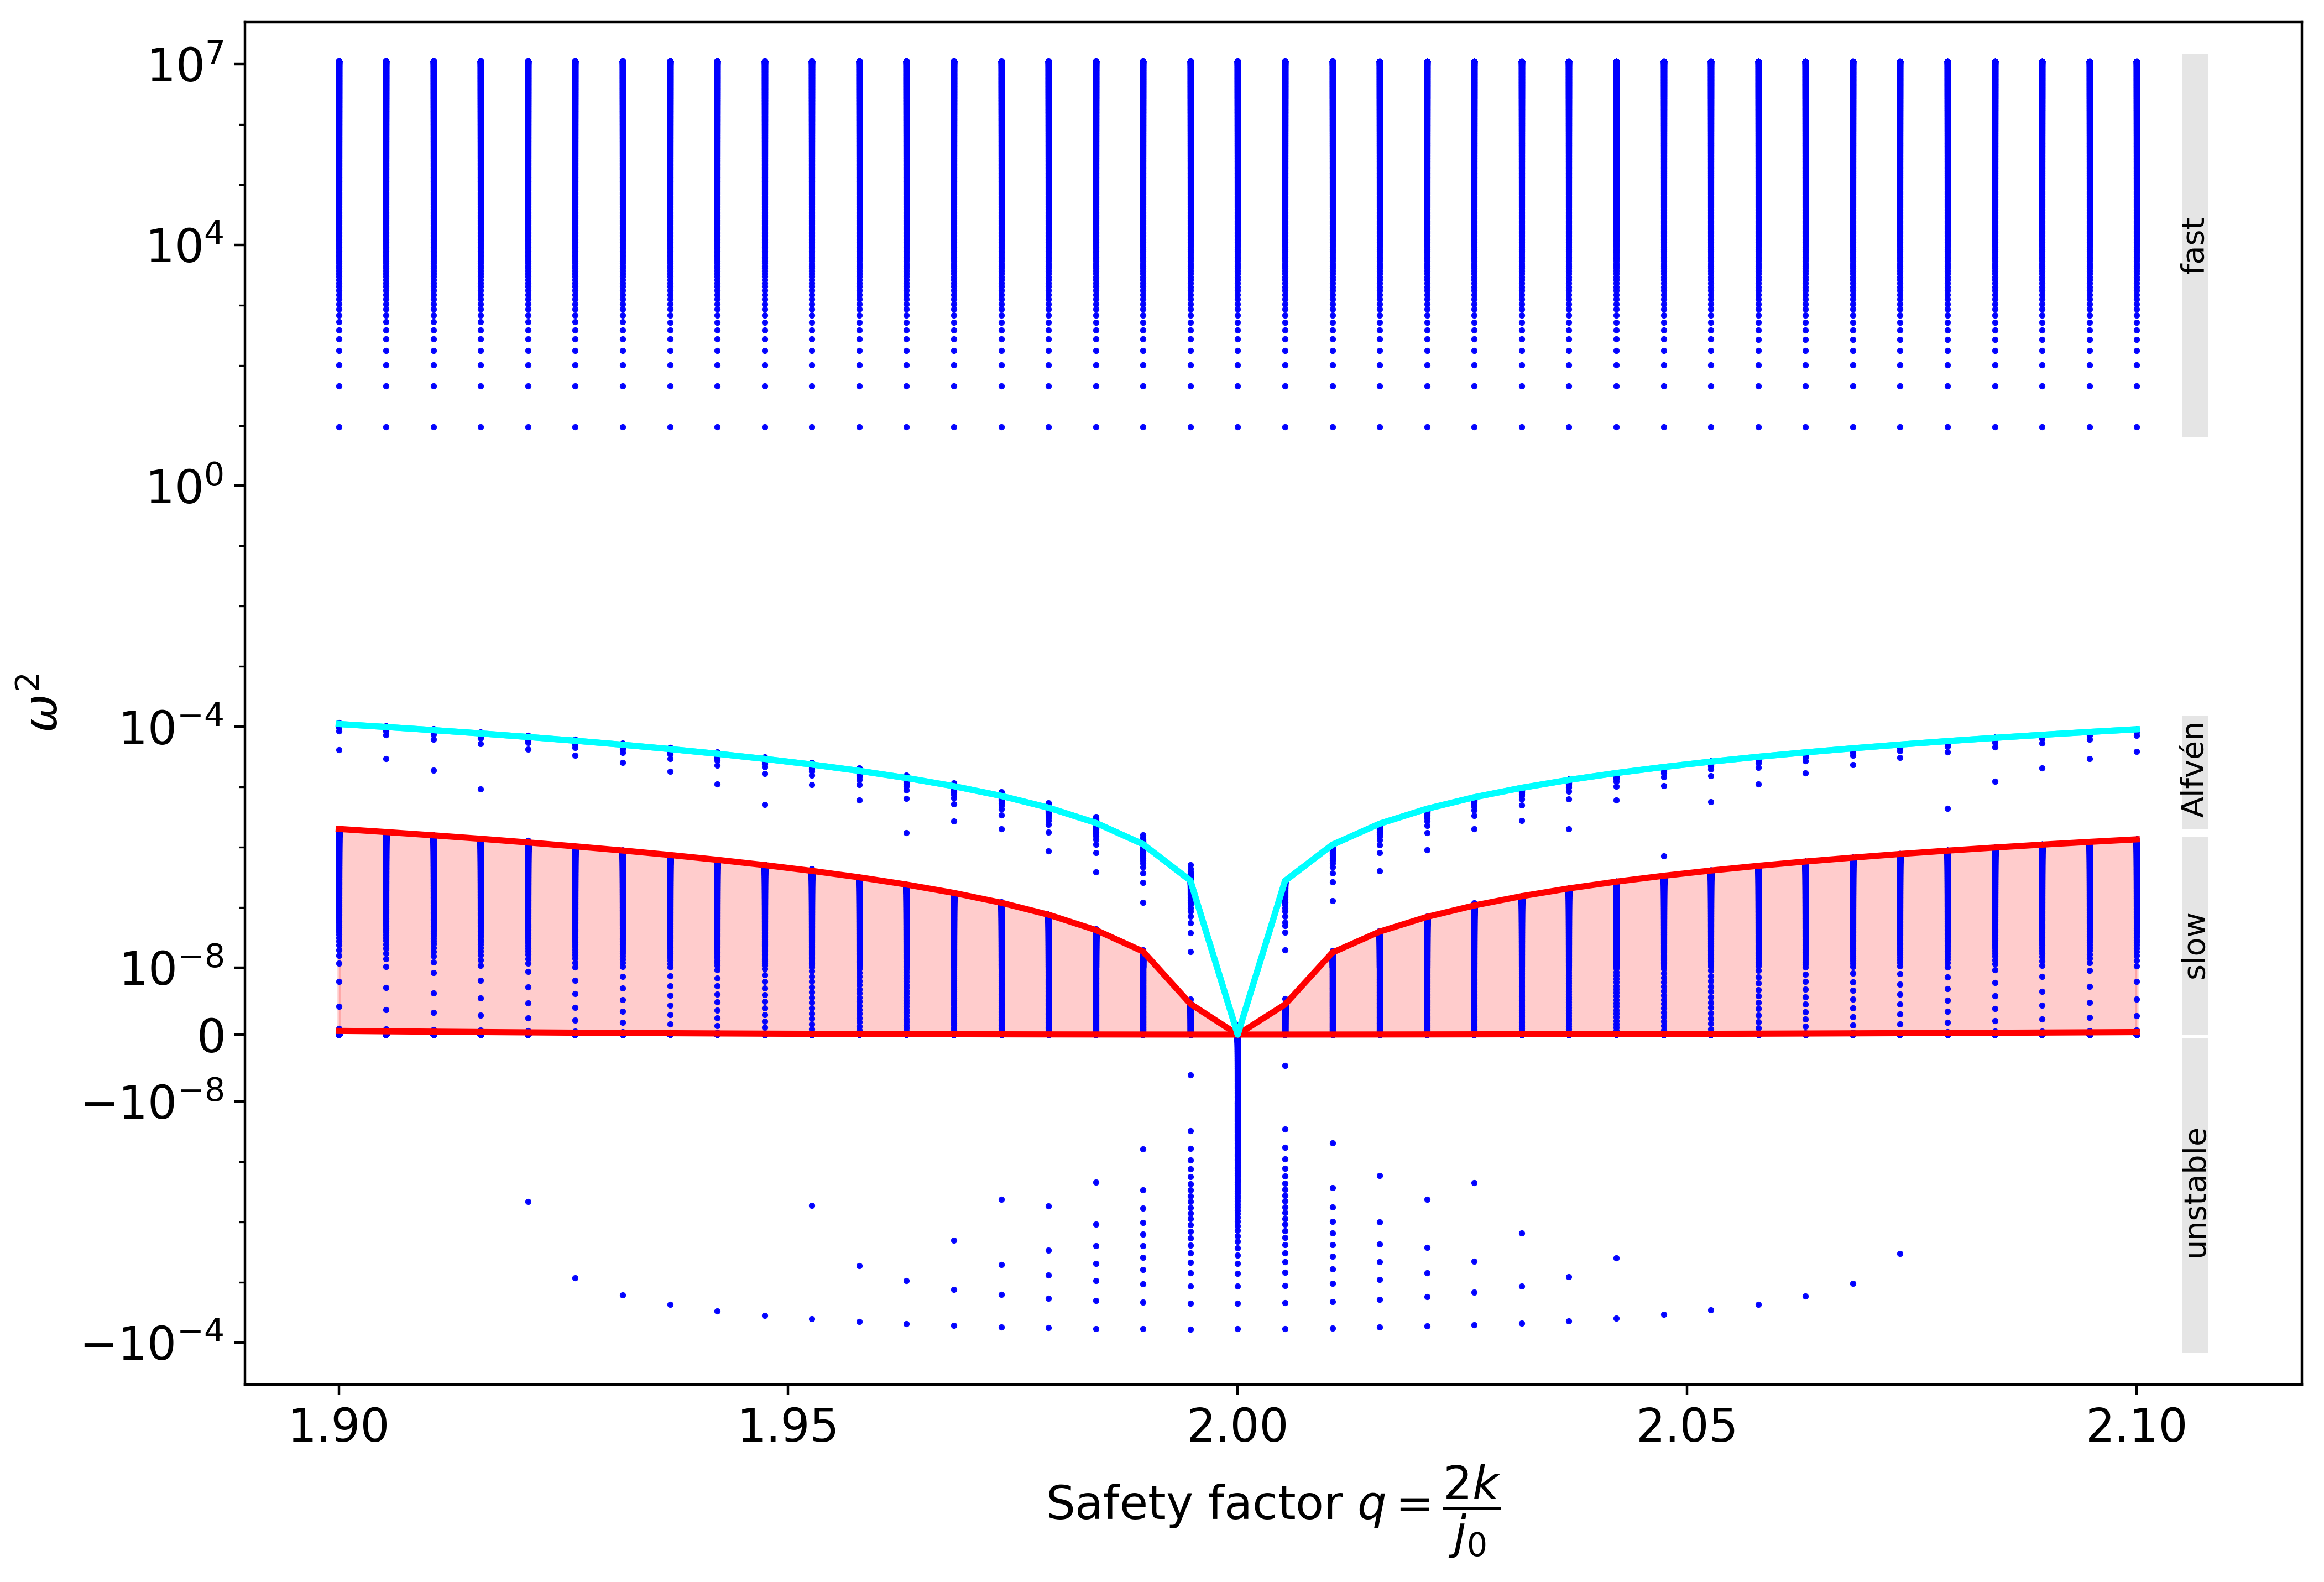
\includegraphics[width=\textwidth]{kerner_tokamak.png}
  \caption{
    Complete MHD spectrum for a tokamak current profile in the presence of the $m = -2$ interchange mode. The squared eigenvalues are plotted against the safety factor $q$, instabilities correspond to $\omega^2 < 0$. The various branches are indicated on the right side of the figure.
  }
  \label{fig: tokamak_current}
\end{figure}

\subsection{KH and CD instabilities} \label{ss: kh_cd_instabilities}
As a first test for the inclusion of flow into the equations, we look at the interaction between the KHIs and current-driven (CD) instabilities in a magnetised astrophysical jet, following \citet{baty2002}. This model uses a cylindrical jet with a supersonic background flow aligned with the axis and sheared in the radial direction. The equilibrium configuration is taken such that Kelvin-Helmholtz surface modes can develop and is generally given by
\begin{equation} \label{eq: kh_cd_equilibrium}
  \begin{gathered}
    \rho_0 = 1,
    \qquad
    v_{02} = 0,
    \qquad
    v_{03} = \frac{1}{2}\mathcal{V}\tanh\left(\frac{r_j - r}{a}\right),
    \qquad
    B_{03} = B_{0z}, \\
    B_{02} = B_{0\theta} \frac{r r_c}{r_c^2 + r^2},
    \qquad
    T_0 = \frac{p_0}{\rho_0} - \frac{B_{0\theta}^2}{2\rho_0}\left(1 - \frac{r_c^4}{\left(r_c^2 + r^2\right)^2}\right).
  \end{gathered}
\end{equation}
Here, $r_j$ denotes the jet radius and $r_c$ quantifies the radial variation, taken to be $r_j = 1$ and $r_c = 0.5$, with $r \in [0, 2]$. The parameter $\mathcal{V}$ represents the amplitude of the velocity, given by $\mathcal{V} = 1.63$, while the chosen velocity profile ensures that the shear layer is situated at the jet radius with a radial width given by $a = 0.1r_j$. Both the density $\rho_0$ and the pressure on-axis $p_0$ are chosen to be equal to unity. The parameters $B_{0\theta}$ and $B_{0z}$ control the amplitude and twist of the magnetic field, as explained in \citet{baty2002}. The original work discusses three different magnetic field configurations, we choose the profile with
\begin{equation}
  B_{0\theta} = 0.4\left(\frac{r_c^2 + r_j^2}{r_j r_c}\right),
  \qquad
  B_{0z} = 0.25,
\end{equation}
such that $B_{02} = 0.4$ at the jet radius. Furthermore, the azimuthal and longitudinal wavenumbers are taken to be $k_2 = m = -1$ and $k_3 = k = \pi$.

The entire spectrum is calculated using 501 gridpoints and shown in Figure \ref{fig: kh_cd}. Panel a depicts the full slow and Alfv\'en spectra with the KH and first three CD unstable modes ($\omega_\text{I} > 0$) denoted on the figure itself. The real and imaginary parts of the $\rho$, $r v_r$, and $v_z$ eigenfunctions for each of these modes are shown on the subsequent panels. Those for the KH mode (Panels c--d) are localised around the jet radius $r = 1$, which is also the point where the Alfv\'enic Mach number drops to zero (Panel b). The quantity $V_0$ in the Figure legend represents the velocity magnitude, here given by $V_0 = \sqrt{v_{02}^2 + v_{03}^2}$. Panels e through j depict the eigenfunctions of the first three CD modes, with the first, second, and third shown in the first, second, and third rows of the bottom panels, respectively. The left column shows the real part, the right column the imaginary part of the eigenfunction. The CD modes have an increasing number of nodes on $r \in [0, 1]$, which is most clearly visible by looking at the
$r v_r$ eigenfunction (green): no nodes for the first CD mode (Panels e--f), one node for the second CD mode (Panels g--h), and two nodes for the third CD mode (Panels i--j).

\begin{figure}[t]
  \centering
  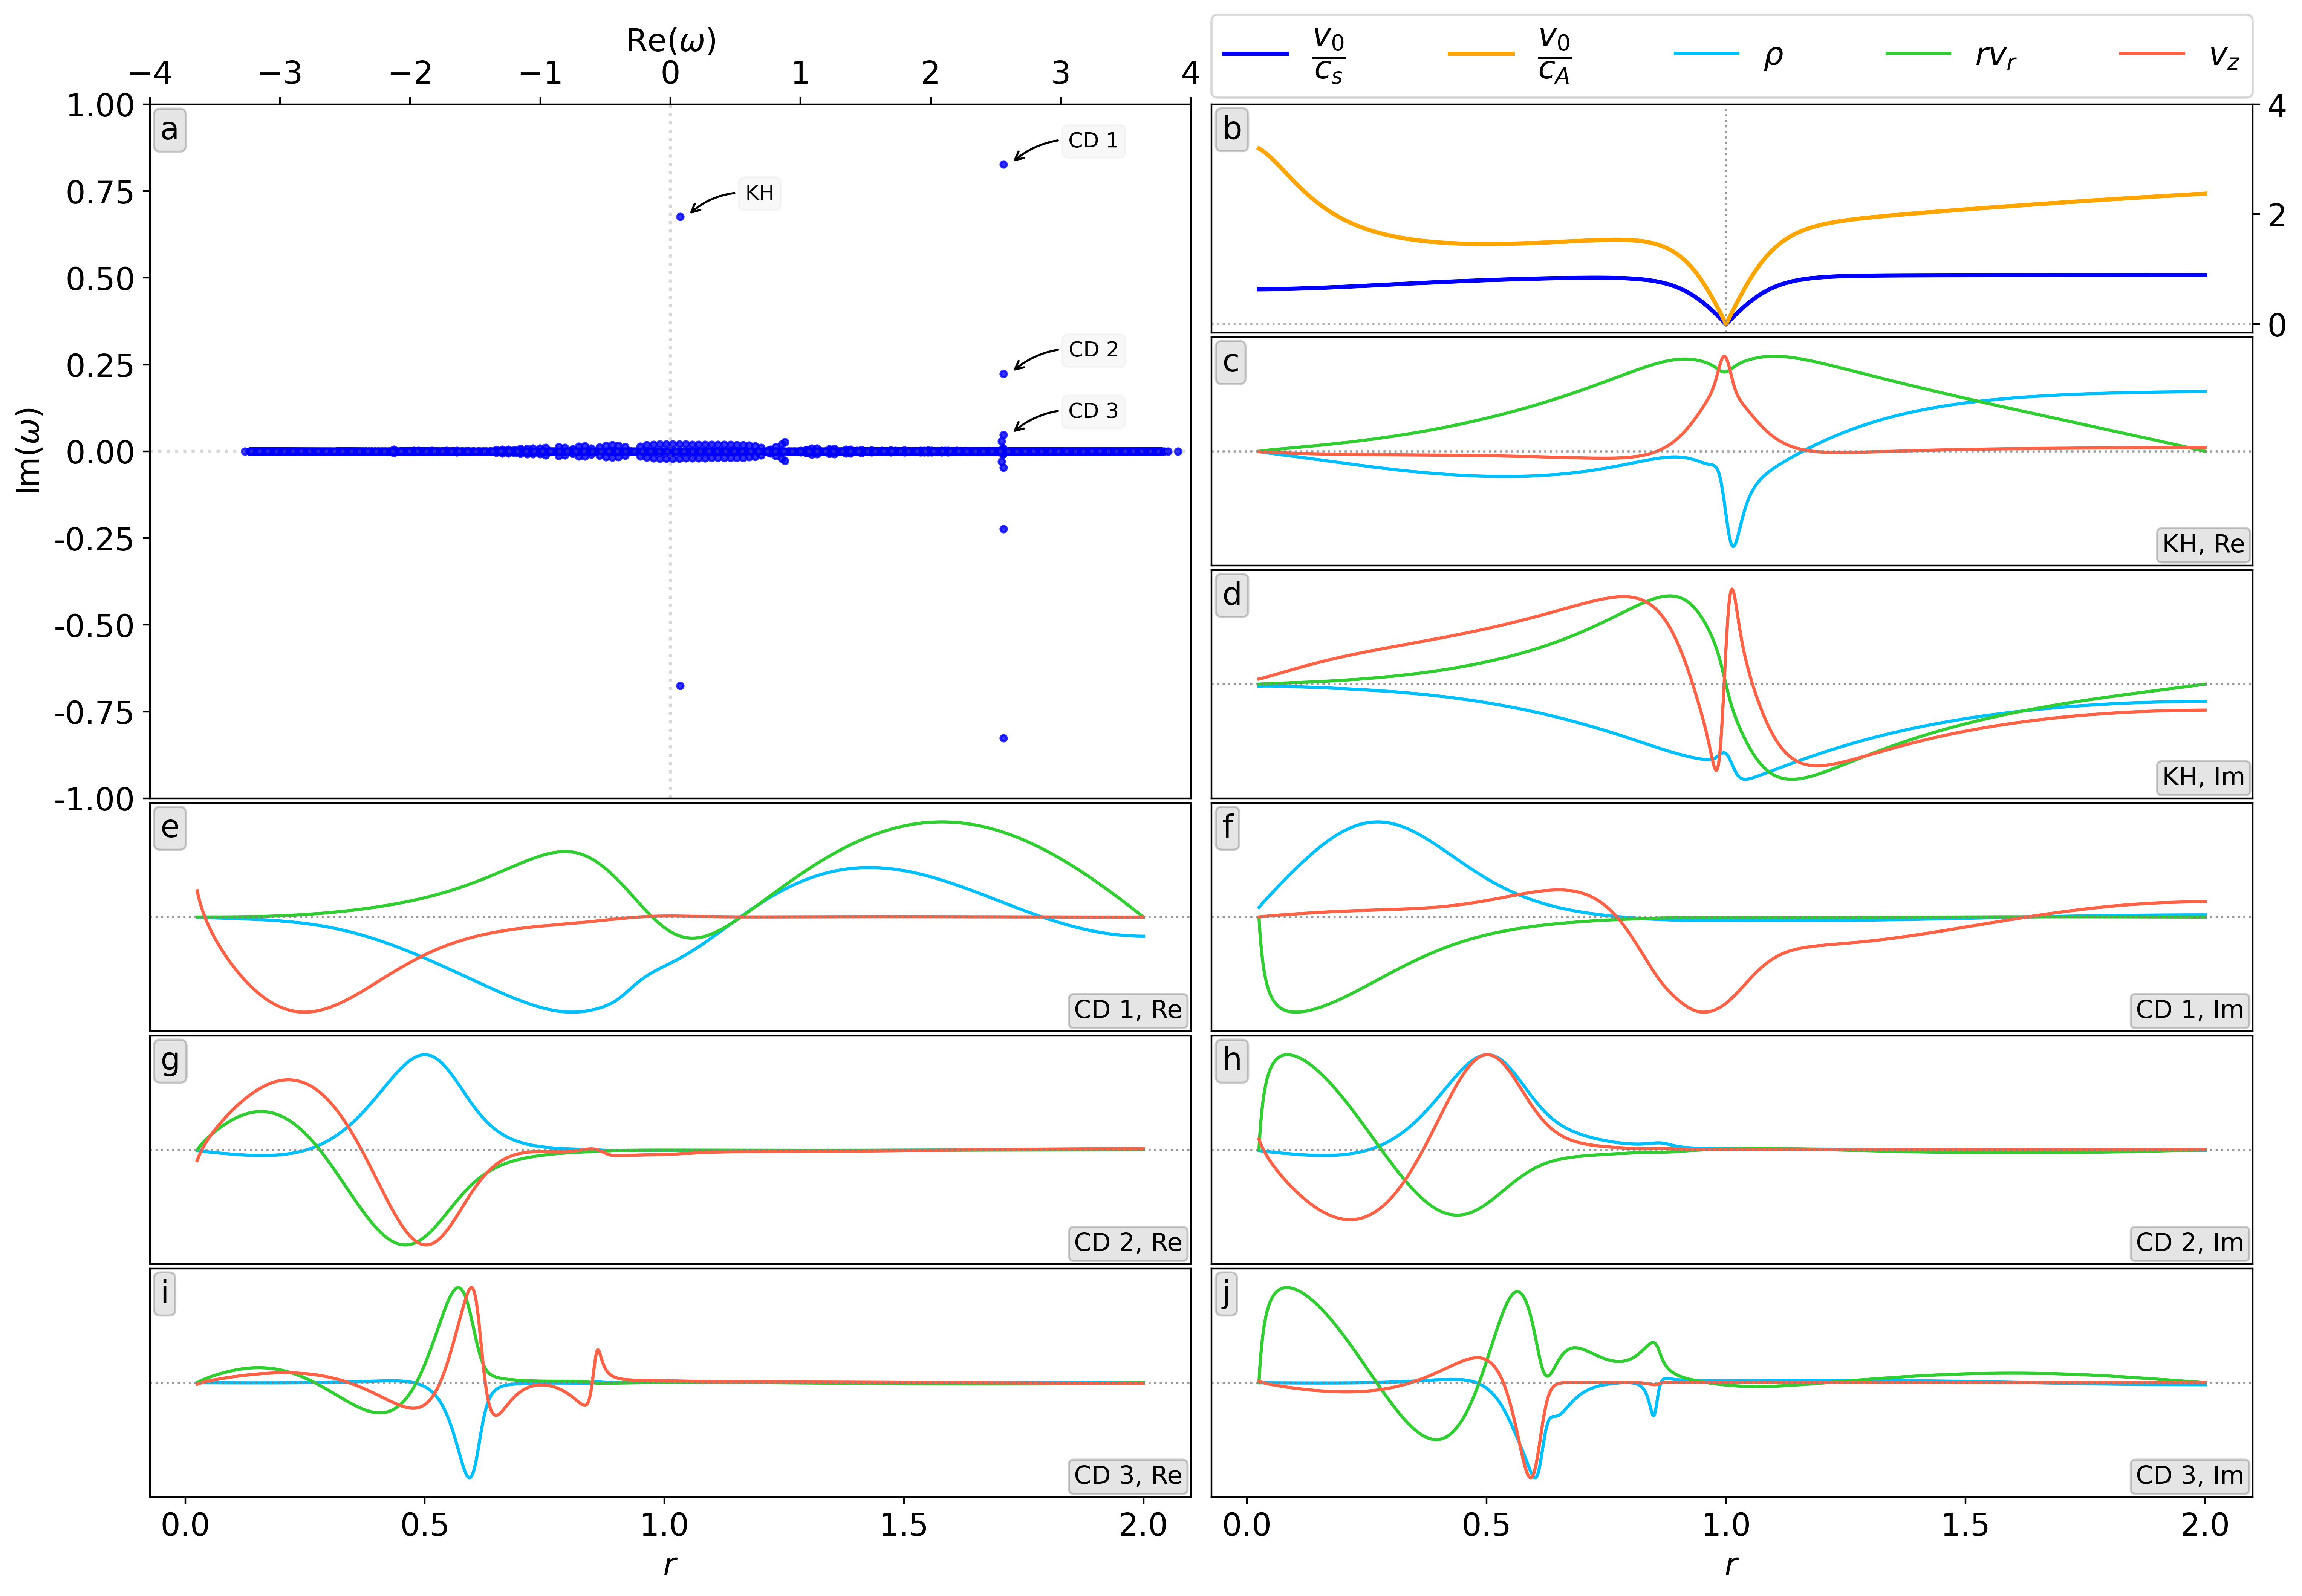
\includegraphics[width=\textwidth]{kh_cd.png}
  \caption{
    Panel \textbf{a}: MHD spectrum for the equilibrium configuration given in \eqref{eq: kh_cd_equilibrium}. The KH and CD instabilities are indicated on the panel. Panel \textbf{b}: sonic and Alfv\'enic Mach numbers; the other panels show the real and imaginary parts of the $\rho$ (blue), $r v_r$ (green) and $v_z$ (red) eigenfunctions, for the KH mode (Panels \textbf{c} and \textbf{d}), first CD mode (Panels \textbf{e}--\textbf{f}), second CD mode (Panels \textbf{g}--\textbf{h}), and third CD mode (Panels \textbf{i}--\textbf{j}).
  }
  \label{fig: kh_cd}
\end{figure}

Note that here, we are still in adiabatic conditions such that the up-down symmetry (relating to time reversal) is still present in the eigenfrequency plane, but the introduction of equilibrium flow caused left-right symmetry breaking between the forwards and backwards propagating modes. As pointed out in \citet{goedbloed2018_web1}, the study of MHD spectra of stationary (i.e. with flow) equilibria is still governed by two self-adjoint operators, but as seen in Figure \ref{fig: kh_cd}, modes can enter the complex plane at various locations (identified by the spectral web \citep{goedbloed2018_web2}). The correspondence with the original figure in \citet{baty2002} is one-to-one for the KH and CD modes, but here we have a lot more detail near the axes due to the (much) higher resolution employed. This resolution aspect will be further discussed in Section \ref{sec: convergence}.

\subsection{Suydam cluster modes}
Next we look at Suydam cluster modes in a cylindrical geometry, which arise from the presence of a Suydam surface in the equilibrium configuration, that is, a location where $\bk \cdot \bb_0 = 0$. Shear flow effects are included, and the equilibrium is given by
\begin{equation} \label{eq: suydam_equilibrium}
  \begin{gathered}
    \rho_0 = 1,
    \qquad
    v_{02} = 0,
    \qquad
    v_{03} = v_{0z}\left(1 - r^2\right),
    \qquad
    B_{02} = J_1(\alpha r), \\
    B_{03} = \sqrt{1 - P_1}J_0(\alpha r),
    \qquad
    p_0 = P_0 + \frac{1}{2}P_1 J_0^2(\alpha r),
  \end{gathered}
\end{equation}
where $\alpha = 2$, $P_0 = 0.05$, $P_1 = 0.1$, and $v_{0z} = 0.14$; the functions $J_0$ and $J_1$ denote the Bessel functions of the first kind. The wavenumbers were chosen to be $k_2 = m = 1$ and $k_3 = k = -1.2$, ensuring a Suydam surface at $r \approx 0.483$.

The spectrum is calculated using 501 gridpoints for $r \in [0, 1]$ and is shown in Figure \ref{fig: suydam_cluster}. The resulting locations of the various off-axis outer modes are in agreement with the results given in \citet{nijboer1997}. However, because this spectrum is calculated using a five times higher resolution, we have much more intricate detail near the Suydam surface, revealing even more off-axis modes (inset in Panel a). The top two panels on the right side of Figure \ref{fig: suydam_cluster} show the sonic and Alfv\'enic Mach numbers (Panel b), together with the $\bk \cdot \bb_0 = B_{02}k_2/r + B_{03}k_3$ and $\bk \cdot \bv_0 = v_{02}k_2/r + v_{03}k_3$ profiles as a function of radius (Panel c), respectively. The location of the Suydam surface at $r \approx 0.483$ is denoted with a red cross.

The bottom row of panels d--g shows the real part of the $\rho$ and $r v_r$ eigenfunctions, for the four modes annotated in Panel a with the location of the Suydam surface indicated with a vertical red line. $\omega_1$ en $\omega_3$ correspond to modes on the left side of the Suydam surface, the other two correspond to modes on the right side. All eigenfunctions shown here show the specific variation associated with their localised behaviour on the left side of the red dashed line, while it is vice versa for the other two modes. For visual purposes the horizontal axis in Panels e and f is different from the one in Panels c and d, because the former correspond to the next modes in the Suydam sequence, showing stronger radial variation. Note that the original Suydam criterion \citep{book_MHD} is related to static equilibria, the generalisation of these Suydam cluster criteria is presented in \citet{wang2004}.

\begin{figure}[t]
  \centering
  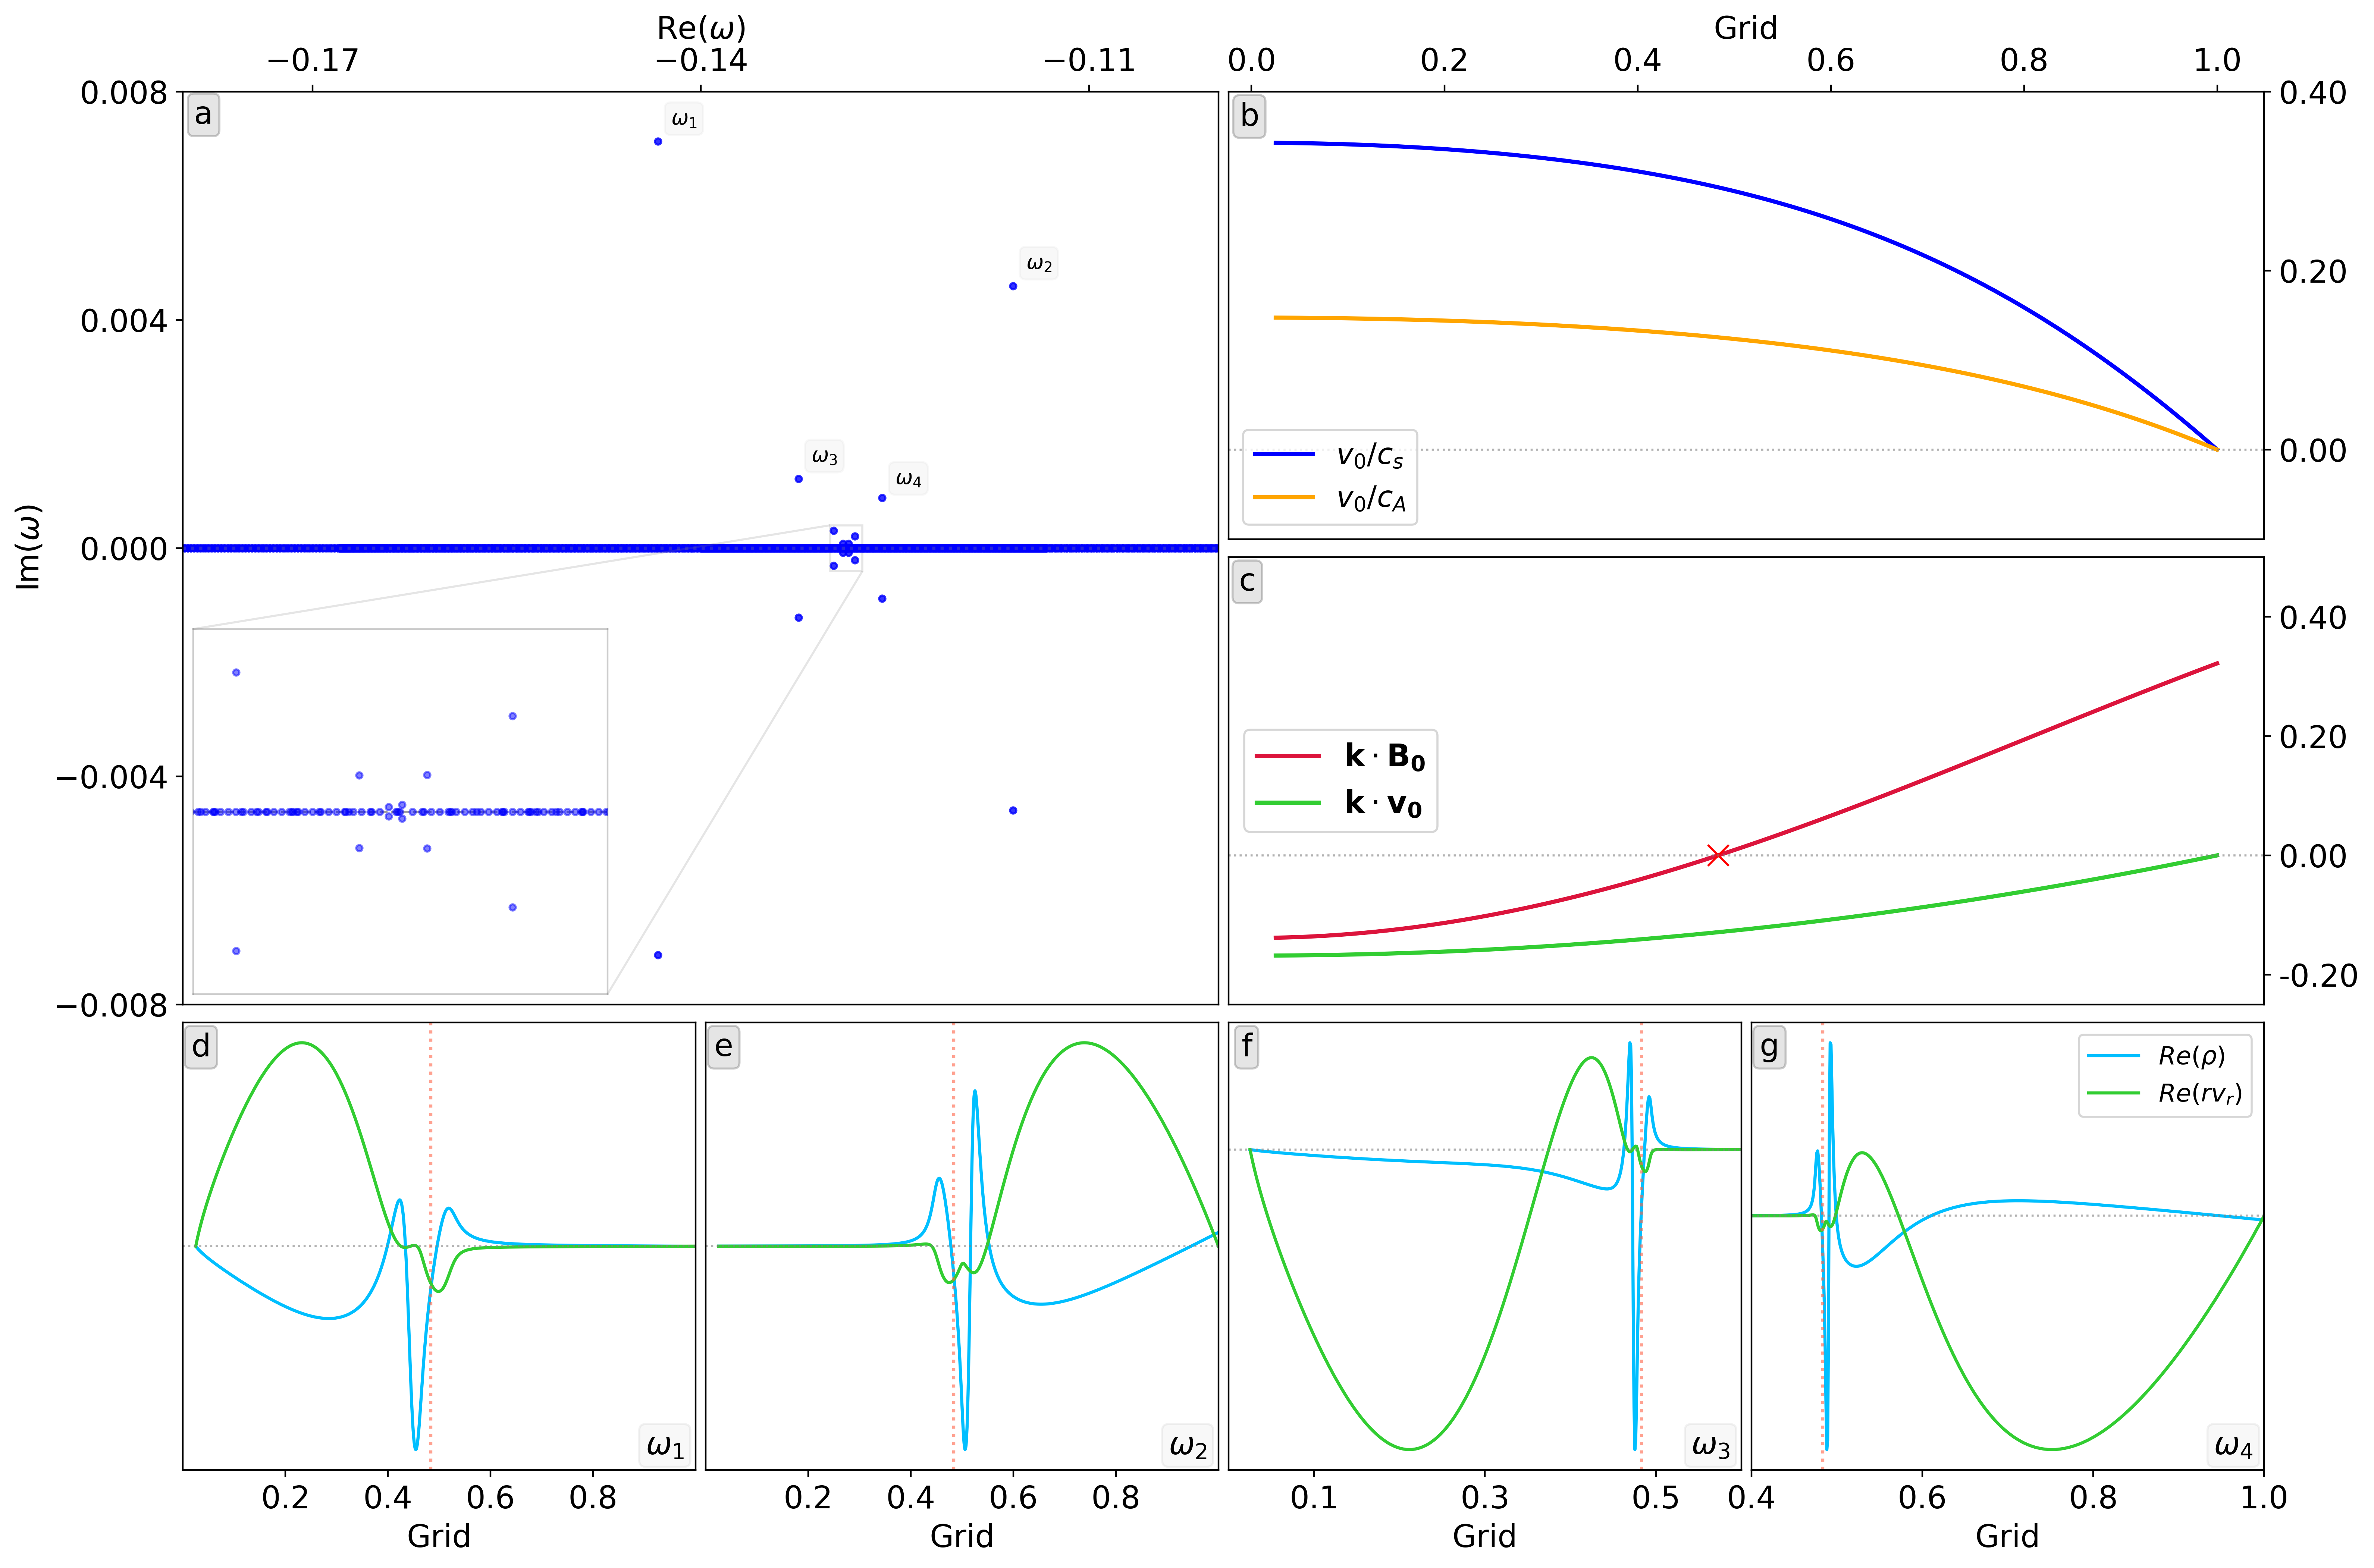
\includegraphics[width=\textwidth]{suydam_cluster.png}
  \caption{
    Panel \textbf{a}: Suydam cluster spectrum for the equilibrium given in \eqref{eq: suydam_equilibrium}. Inset: zoom-in near the Suydam surface, revealing more detail. Panel \textbf{b} depicts the sonic and Alfv\'enic Mach numbers as a function of radius, Panel \textbf{c} shows the $\bk \cdot \bb_0$ and $\bk \cdot \bv_0$ curves where the red cross denotes the Suydam surface. The bottom row of panels shows the real part of the $\rho$ and $r v_r$ eigenfunctions, for the four modes in the Suydam sequence annotated in Panel \textbf{a}. The dotted red line denotes the location of the Suydam surface.
  }
  \label{fig: suydam_cluster}
\end{figure}



\section{Resistive, Cartesian cases}
All cases discussed up to now handles an adiabatic equilibrium configuration with or without the inclusion of flow. The up-down symmetry of all the MHD spectra shown so far is perfectly maintained, related to the fact that these cases are in essence time-reversible. Every instability (or overstability in the case of flow) has a damped counterpart. We now move on to include additional effects, that is, we now calculate spectra for time-irreversible cases, where either resistivity or non-adiabatic effects enter, which will break the up-down symmetry. We first focus on the inclusion of resistivity.


\subsection{Resistive homogeneous plasmas}
To start with we take a look at the simplest configuration, that is, a homogeneous plasma in a Cartesian geometry with resistivity included. The uniform equilibrium is given by
\begin{equation} \label{eq: resistive_homo_equilibrium}
  \rho_0 = 1,
  \qquad
  B_{02} = 0,
  \qquad
  B_{03} = 1,
  \qquad
  T_0 = \frac{1}{2}\beta B_0^2
\end{equation}
where we take a plasma beta of $\beta = 0.25$, $k_2 = k_y = 0$, $k_3 = k_z = 1$, and $x \in [0, 1]$. The value for the resistivity is assumed to be constant and given by $\eta = 10^{-3}$, as described in \citet{book_MHD}. This spectrum is calculated using 1001 gridpoints; the result is shown in Figure \ref{fig: resistive_homo}. In ideal MHD the fast modes form a Sturmian sequence (that is, the oscillation of the eigenfrequencies increases then the number of modes increases, which in turn implies a larger real part of $\omega$) of stable fast magnetoacoustic waves with frequencies accumulating to infinite frequency (related to the $p$ modes in our stratified example). The slow modes have an anti-Sturmian sequence toward their accumulation point (in essence the collapsed slow continuum) and the Alfv\'en modes are degenerate \citep{book_MHD}. When resistivity is included, the fast modes become damped and the Alfv\'en and slow modes trace out semicircles on the bottom-half of the complex plane. The semicircles and initial fast-mode sequence shown in Figure \ref{fig: resistive_homo} are in perfect agreement with the spectrum depicted in \citet[Figure 14.6]{book_MHD}. These semicircles can be quantified analytically; their radius does not depend on resistivity. The magnetic Reynolds number, calculated as $\magneticreynolds = (x_1 - x_0)\alfvenspeed / \eta$, is equal to 1000.

Due to the rather extreme resolution employed here, we trace much further into the fast-mode sequence, where we see something interesting: the fast modes appear on curves that loop around, breaking the purely Sturmian behaviour for a moment, after which they continue again toward infinity. This implies that initially, the fast modes become more damped at higher mode frequencies up to a certain turning point at which they achieve maximal damping (the bottom of the loop). After passing this turning point, the oscillation frequency of the modes increases again and the damping frequency seems to converge toward one single value.

Of course, the strong damping for the fast modes as we go further into the fast-mode sequence must have consequences for the original uniform (ideal) equilibrium state. In what follows, we will adopt the common practice of computing resistive MHD spectra about an ideal MHD state, which itself will evolve when resistivity is acting. This is directly related to the discussion on the equilibrium background in Section \ref{ss: equilibrium conditions} when resistivity is taken into account.

\begin{figure}[t]
  \centering
  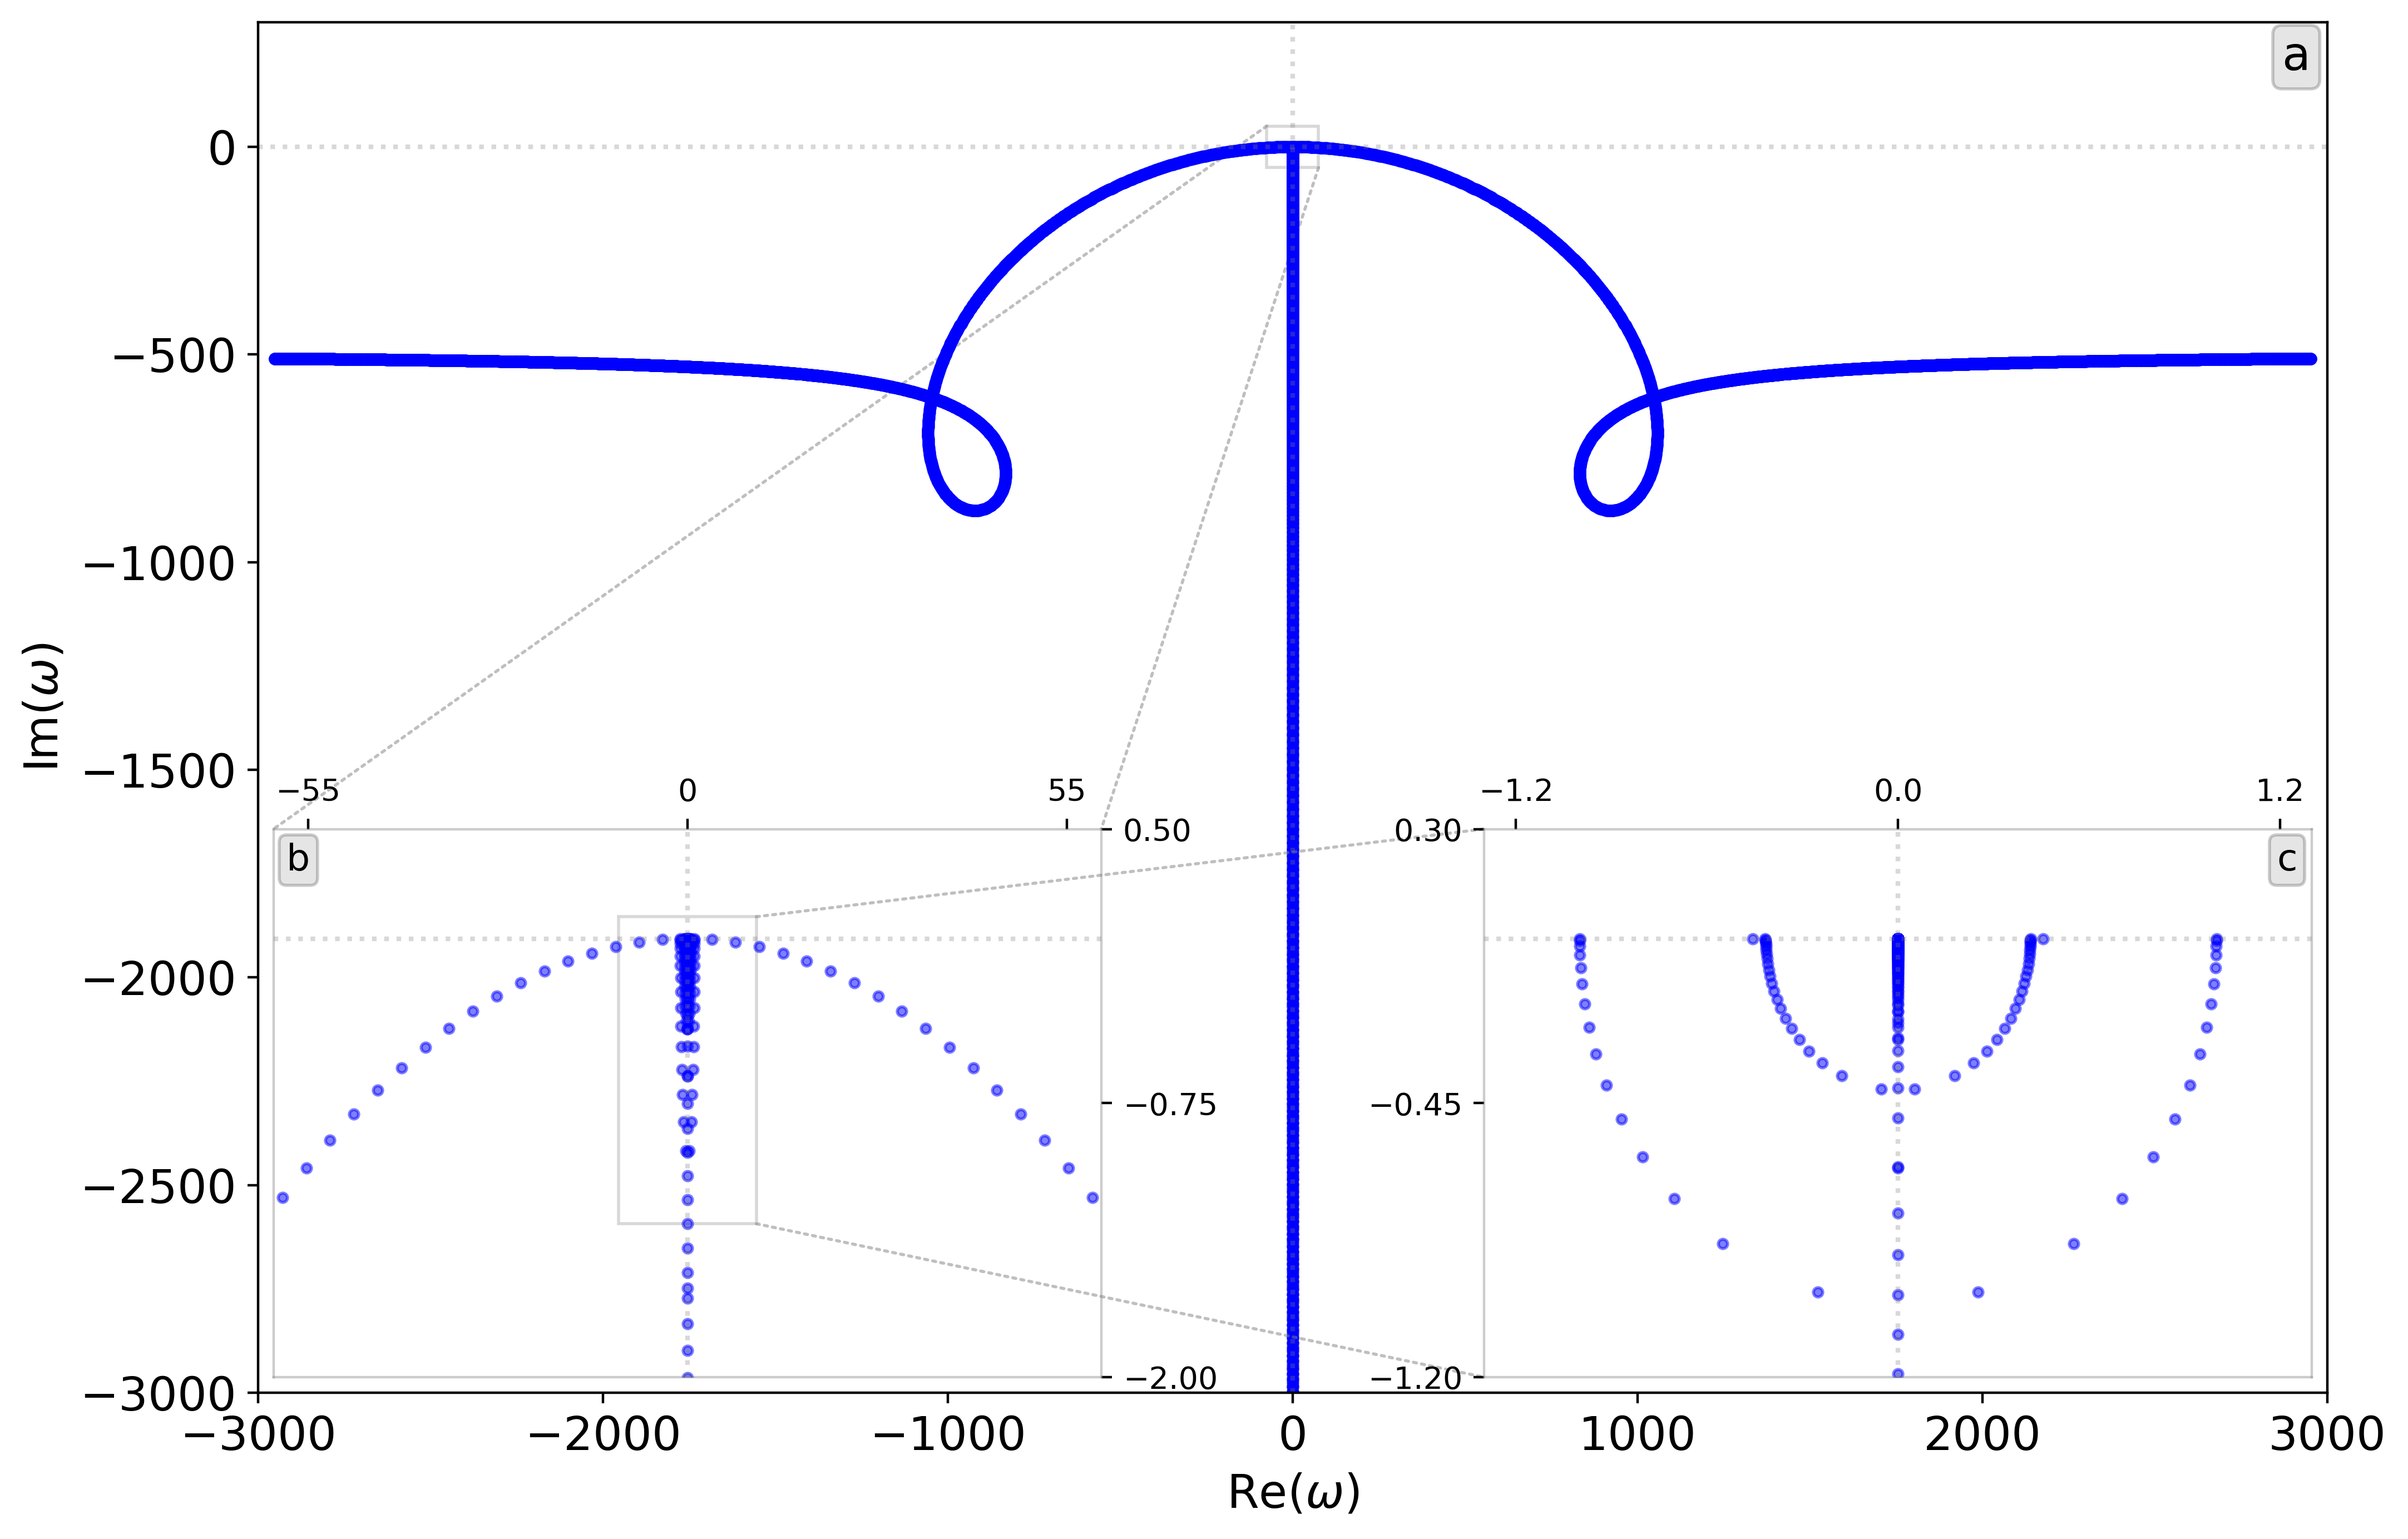
\includegraphics[width=\textwidth]{resistive_homo.png}
  \caption{
    Panel \textbf{a}: spectrum for a homogeneous medium with constant resistivity. Panel \textbf{b} zooms in near the origin, showing the start of the fast-mode sequence. Panel \textbf{c} zooms in further, revealing the semicircles traced out by the Alfv\'en and slow modes (outer and inner semicircles, respectively).
  }
  \label{fig: resistive_homo}
\end{figure}


\subsection{Quasi-modes in resistive MHD}
We now turn to a nonadiabatic case, where resistivity is important. We will compute the resistive MHD spectrum for a case where the equilibrium varies across an interface, which gives rise to so-called quasi-modes. These are essentially surface waves undergoing damping, due to the fact that the global quasi-mode overlaps in frequency with the continuum range, causing resonant absorption. Quasi-modes are quite important in solar physics, as they can be indirectly related to the coronal heating problem as discussed in, for example, \citet{poedts1989} and \citet{poedts1991}.

A detailed analytical treatment of quasi-modes including theoretical growth rates is given in \citet{book_priest}, where they start from an inhomogeneous layer of width $l$ connecting two regions of uniform plasma. This can be reproduced by introducing a linear density profile between two homogeneous regions in a Cartesian geometry, however, this would mean that the density derivative shows rather strong discontinuities near the edges of the transition layer. Similar to \citet{ruderman2002} we therefore opt for a smooth profile by introducing a sine dependence such that

\begin{equation}
  \rho_0(x) =
  \begin{cases}
    \rho_1 &\text{if}~x_0 \leq x < s - \dfrac{1}{2}l, \\
    \dfrac{1}{2}\rho_1\left[
      1 + \dfrac{\rho_2}{\rho_1} - \left(1 - \dfrac{\rho_2}{\rho_1}\right)\sin\left(\dfrac{\pi(x - s)}{l}\right)
    \right] &\text{if}~s - \dfrac{1}{2}l \leq x \leq s + \dfrac{1}{2}l, \\
    \rho_2 &\text{if}~s + \dfrac{1}{2}l < x \leq x_1,
  \end{cases}
\end{equation}
where $s$ denotes the midpoint between $x_0$ and $x_1$, representing the left and right edges of the Cartesian grid, respectively, and equal to $0$ and $1$ such that $s = 0.5$. The width of the transition region $l = 0.1$ is taken to be small as to reduce the influence of the walls. If $l \rightarrow 0$, the inhomogeneous region disappears, and we simply have a discontinuous jumpy in the plasma. Furthermore, we take $\rho_1 = 0.9$, $\rho_2 = 0.1$, $B_{02} = 0$, $B_{03}$ = 1, and $T_0 = 0$. The magnetic field is unidirectional along the $z$-axis, and setting the temperature (and thus pressure) to zero provides an additional test on the handling of zero rows in the matrix. This zero-temperature case is frequently encountered in fully nonlinear MHD simulations which artificially adopt a zero plasma beta. It has as an important consequence that the slow continuum collapses to marginal frequency, eliminating many interesting modes from the spectrum. Additionally, we adopt wavenumbers $k_3 = 0.05$ and $k_2 = 1$, such that $k_3 \ll k_2$. As discussed in \citet{book_priest}, the quasi-modes are damped, such that they move away from the real eigenfrequency axis with complex eigenvalues $\omega = \omega_\text{R} + \icomplex \omega_\text{I}$ given by
\begin{equation} \label{eq: quasimode}
  \omega_\text{R} = \pm \sqrt{\frac{\rho_1 \omega_\text{A1}^2 + \rho_2 \omega_\text{A2}^2}{\rho_1 + \rho_2}},
  \qquad
  \omega_\text{I} = -\frac{\pi k_z l \left(\omega_\text{A2}^2 - \omega_\text{A1}^2\right)}{8\omega_\text{R}},
\end{equation}
with $\omega_\text{A}^2 = k_z^2 \alfvenspeed^2$. This analytic result originates from a complex analysis of the linearised initial value problem. However, there is one caveat: it is impossible to obtain complex eigenvalues away from the real or imaginary axis in an ideal plasma, due to the matrix operator being Hermitian in ideal MHD. Because the (ideal) quasi-mode is damped, we therefore include a (small) value for the resistivity, $\eta = 10^{-4}$, which is sufficient to make the matrix operator non-Hermitian and allows for complex eigenvalues away from the horizontal axis.

\begin{figure}[t]
  \centering
  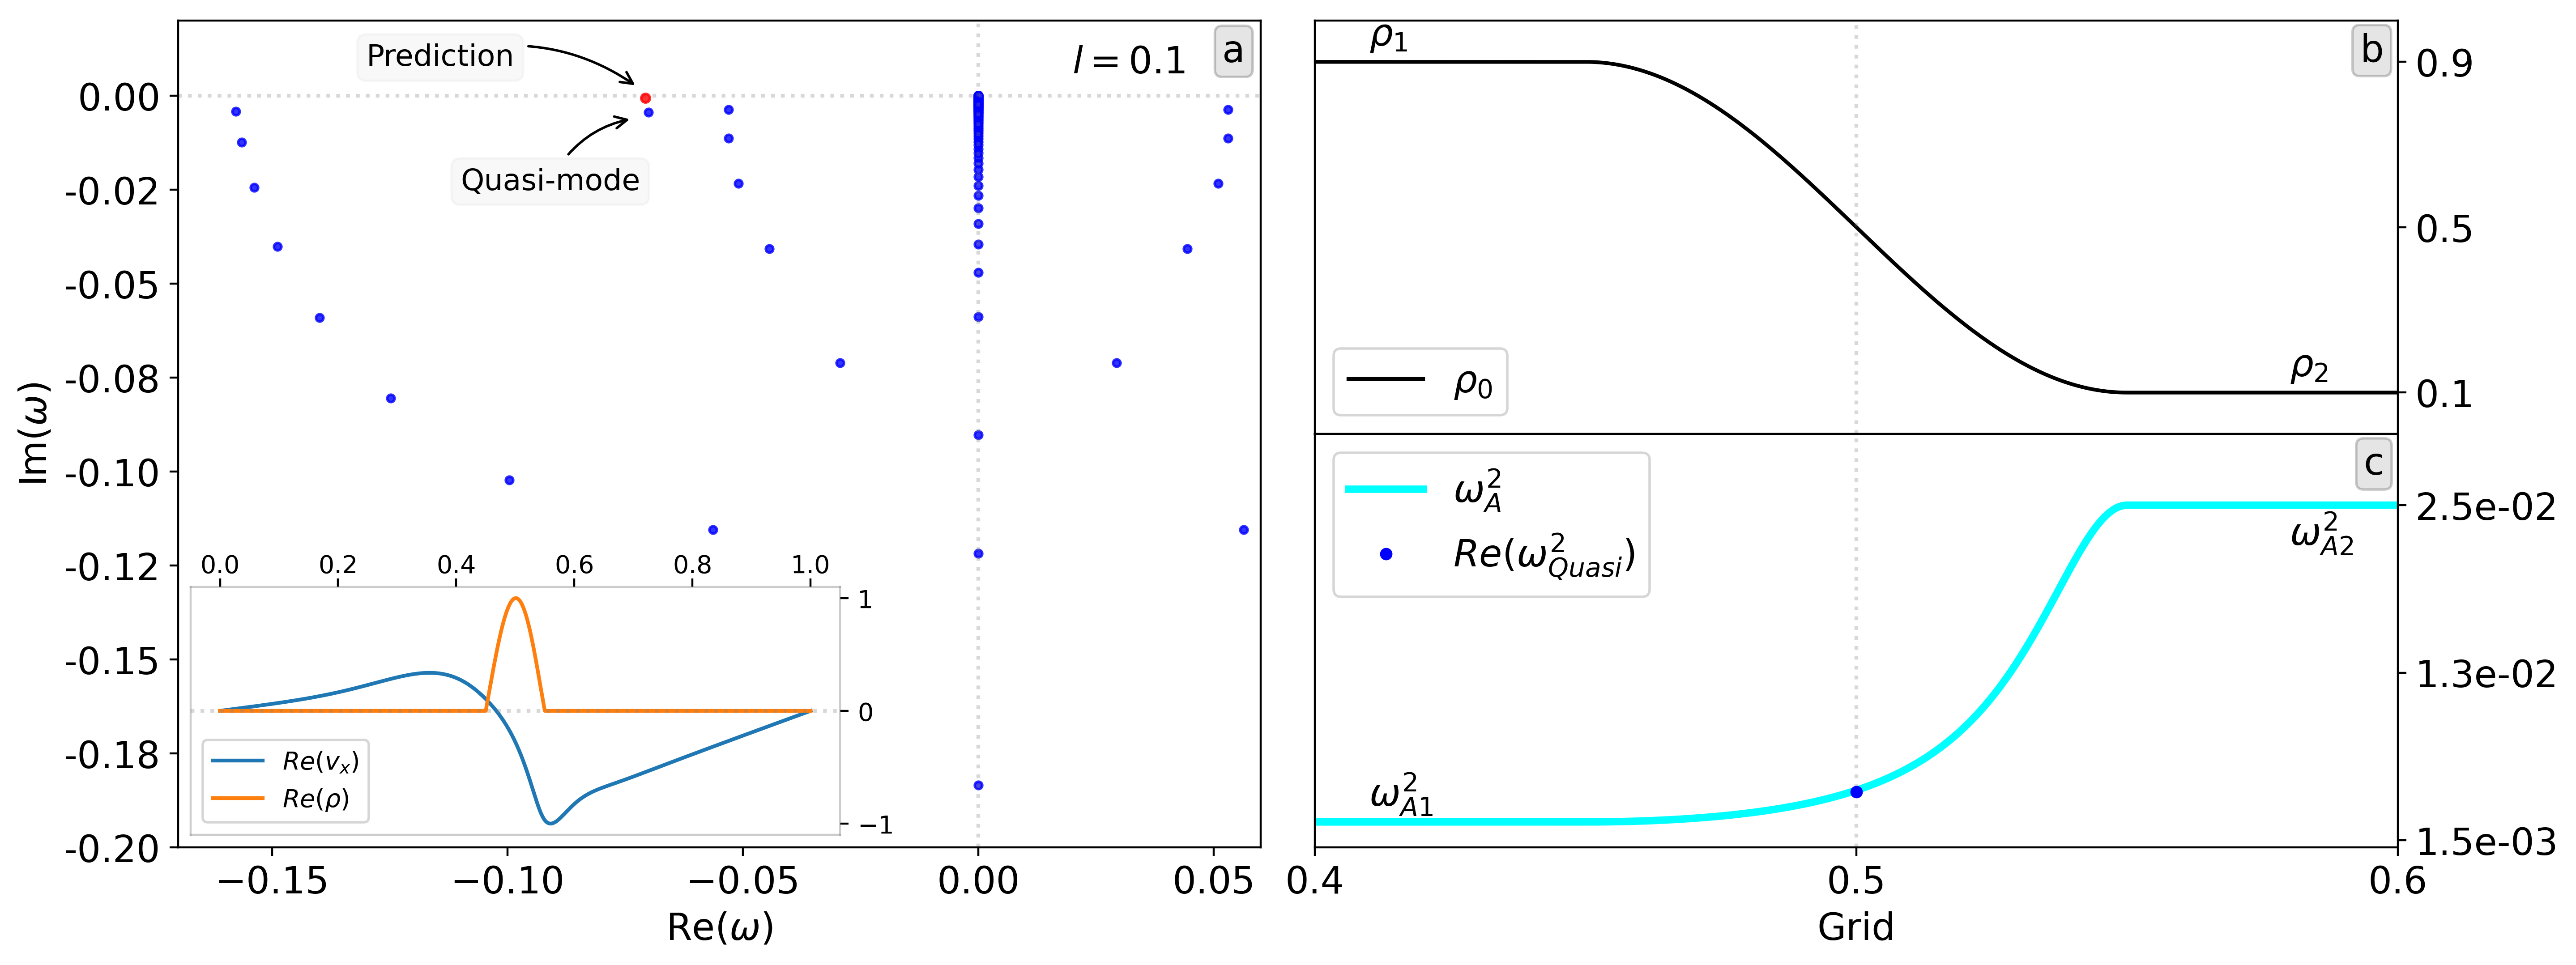
\includegraphics[width=\textwidth]{quasimodes.png}
  \caption{
    Panel \textbf{a}: part of the MHD spectrum containing the quasi-mode, the red dot denotes the theoretical prediction of Equation \eqref{eq: quasimode}. Panels \textbf{b} and \textbf{c} show plots of the sinusoidal density profile and Alfv\'en frequency as a function of the grid, respectively. Note that these two panels only show part of the grid, near the transition region. The inset shows the real part of the $v_x$ (orange) and $\rho$ (blue) normalised eigenfunctions associated with the quasi-mode. The blue dot in Panel \textbf{c} denotes the squared quasi-mode frequency, matching the squared Alfv\'en frequency at $x = 0.5$. The vertical dotted line denotes the middle of the grid.
  }
  \label{fig: quasimodes}
\end{figure}


The magnetic Reynolds number in this case varies between $\magneticreynolds \approx 10^4$ and $\magneticreynolds \approx 3 \times 10^4$. Figure \ref{fig: quasimodes} shows the MHD spectrum in Panel a, for 501 gridpoints, with the theoretical prediction for the global quasi-mode location annotated with a red dot. The actual quasi-mode is also denoted in the figure and is slightly more damped than its theoretical counterpart. This is to be expected, because the inclusion of resistivity imposed additional damping on the eigenvalues, shifting them downwards. It should be noted that increasing the with $l$ of the transition layer moves the quasi-mode farther down and to the right in the figure, such that it eventually merges with the damped modes found on the branch immediately to its right. This phenomenon, where the quasi-modes merge with the resistive branches, is discussed in more detail in \citet{vandoorsselaere2007}. The inset in Panel a depicts the $\rho$ (blue) and $v_x$ (orange) eigenfunctions associated with the quasi-mode, showing localised variation near the transition region as expected. Note that the spectrum as shown in Figure \ref{fig: quasimodes}, left Panel a, is still left-right symmetric, but that resistivity has broken the up-down symmetry, with all modes here found in the stable (damped) half plane.


\subsection{Resistive tearing modes}
Now we move on to an inhomogeneous medium with the inclusion of resistivity and an optional linear flow profile, discussed in \citet{book_MHD}. The geometry is Cartesian, with $x \in [-0.5, 0.5]$ and an equilibrium configuration given by
\begin{equation} \label{eq: resistive_tearing}
  \begin{gathered}
    \rho_0 = 1,
    \qquad
    B_{02} = \sin(\alpha x),
    \qquad
    B_{03} = \cos(\alpha x), \\
    T_0 = \frac{1}{2}\beta B_0^2,
    \qquad
    v_{02} = \mathcal{V}x,
    \qquad
    v_{03} = 0,
  \end{gathered}
\end{equation}
where $k_3 = k_z = 0$, $\beta = 0.15$, and $\alpha = 4.73884$, with a constant resistivity value of $\eta = 10^{-4}$. The magnetic configuration chosen here is a linear force-free field with shear, where $\alpha$ is the proportionality constant between the current and magnetic field, that is, $\boldsymbol{j_0} = \alpha \bb_0$. This specific choice of parameters violates the tearing mode stability criterion \citep{book_MHD}, which results in an isolated, unstable tearing mode. Spectra are calculated both for $\mathcal{V} = 0$ (no flow) and $\mathcal{V} = 0.15$, the inclusion of a linear velocity profile in the latter case introduces a Doppler shift in the slow and Alfv\'en continua, and the results are shown for 501 gridpoints in Figure \ref{fig: resistive_tearing}. Panels a and b show spectra for
$\mathcal{V} = 0$, $k_2 = k_y = 0.49$ (no flow) and $\mathcal{V} = 0.15$, $k_y = 1.5$ (linear flow profile), respectively, revealing the intricate behaviour of the damped slow and Alfv\'en sequences. The purely imaginary unstable tearing mode is annotated with an arrow. The resistivity $\eta$ is equal to $10^{-4}$ for both cases, yielding a magnetic Reynolds number of $\magneticreynolds \approx 10^4$. These results are in perfect agreement with the original spectra depicted in \citet[Figures 14.7--14.9]{book_MHD}. Note that these cases still have left-right symmetry maintained, despite the presence of equilibrium flow. However, this is purely because the flow profile and domain happen to be chosen in a symmetric way, such that forward and backward modes behave symmetrically.

\begin{figure}[t]
  \centering
  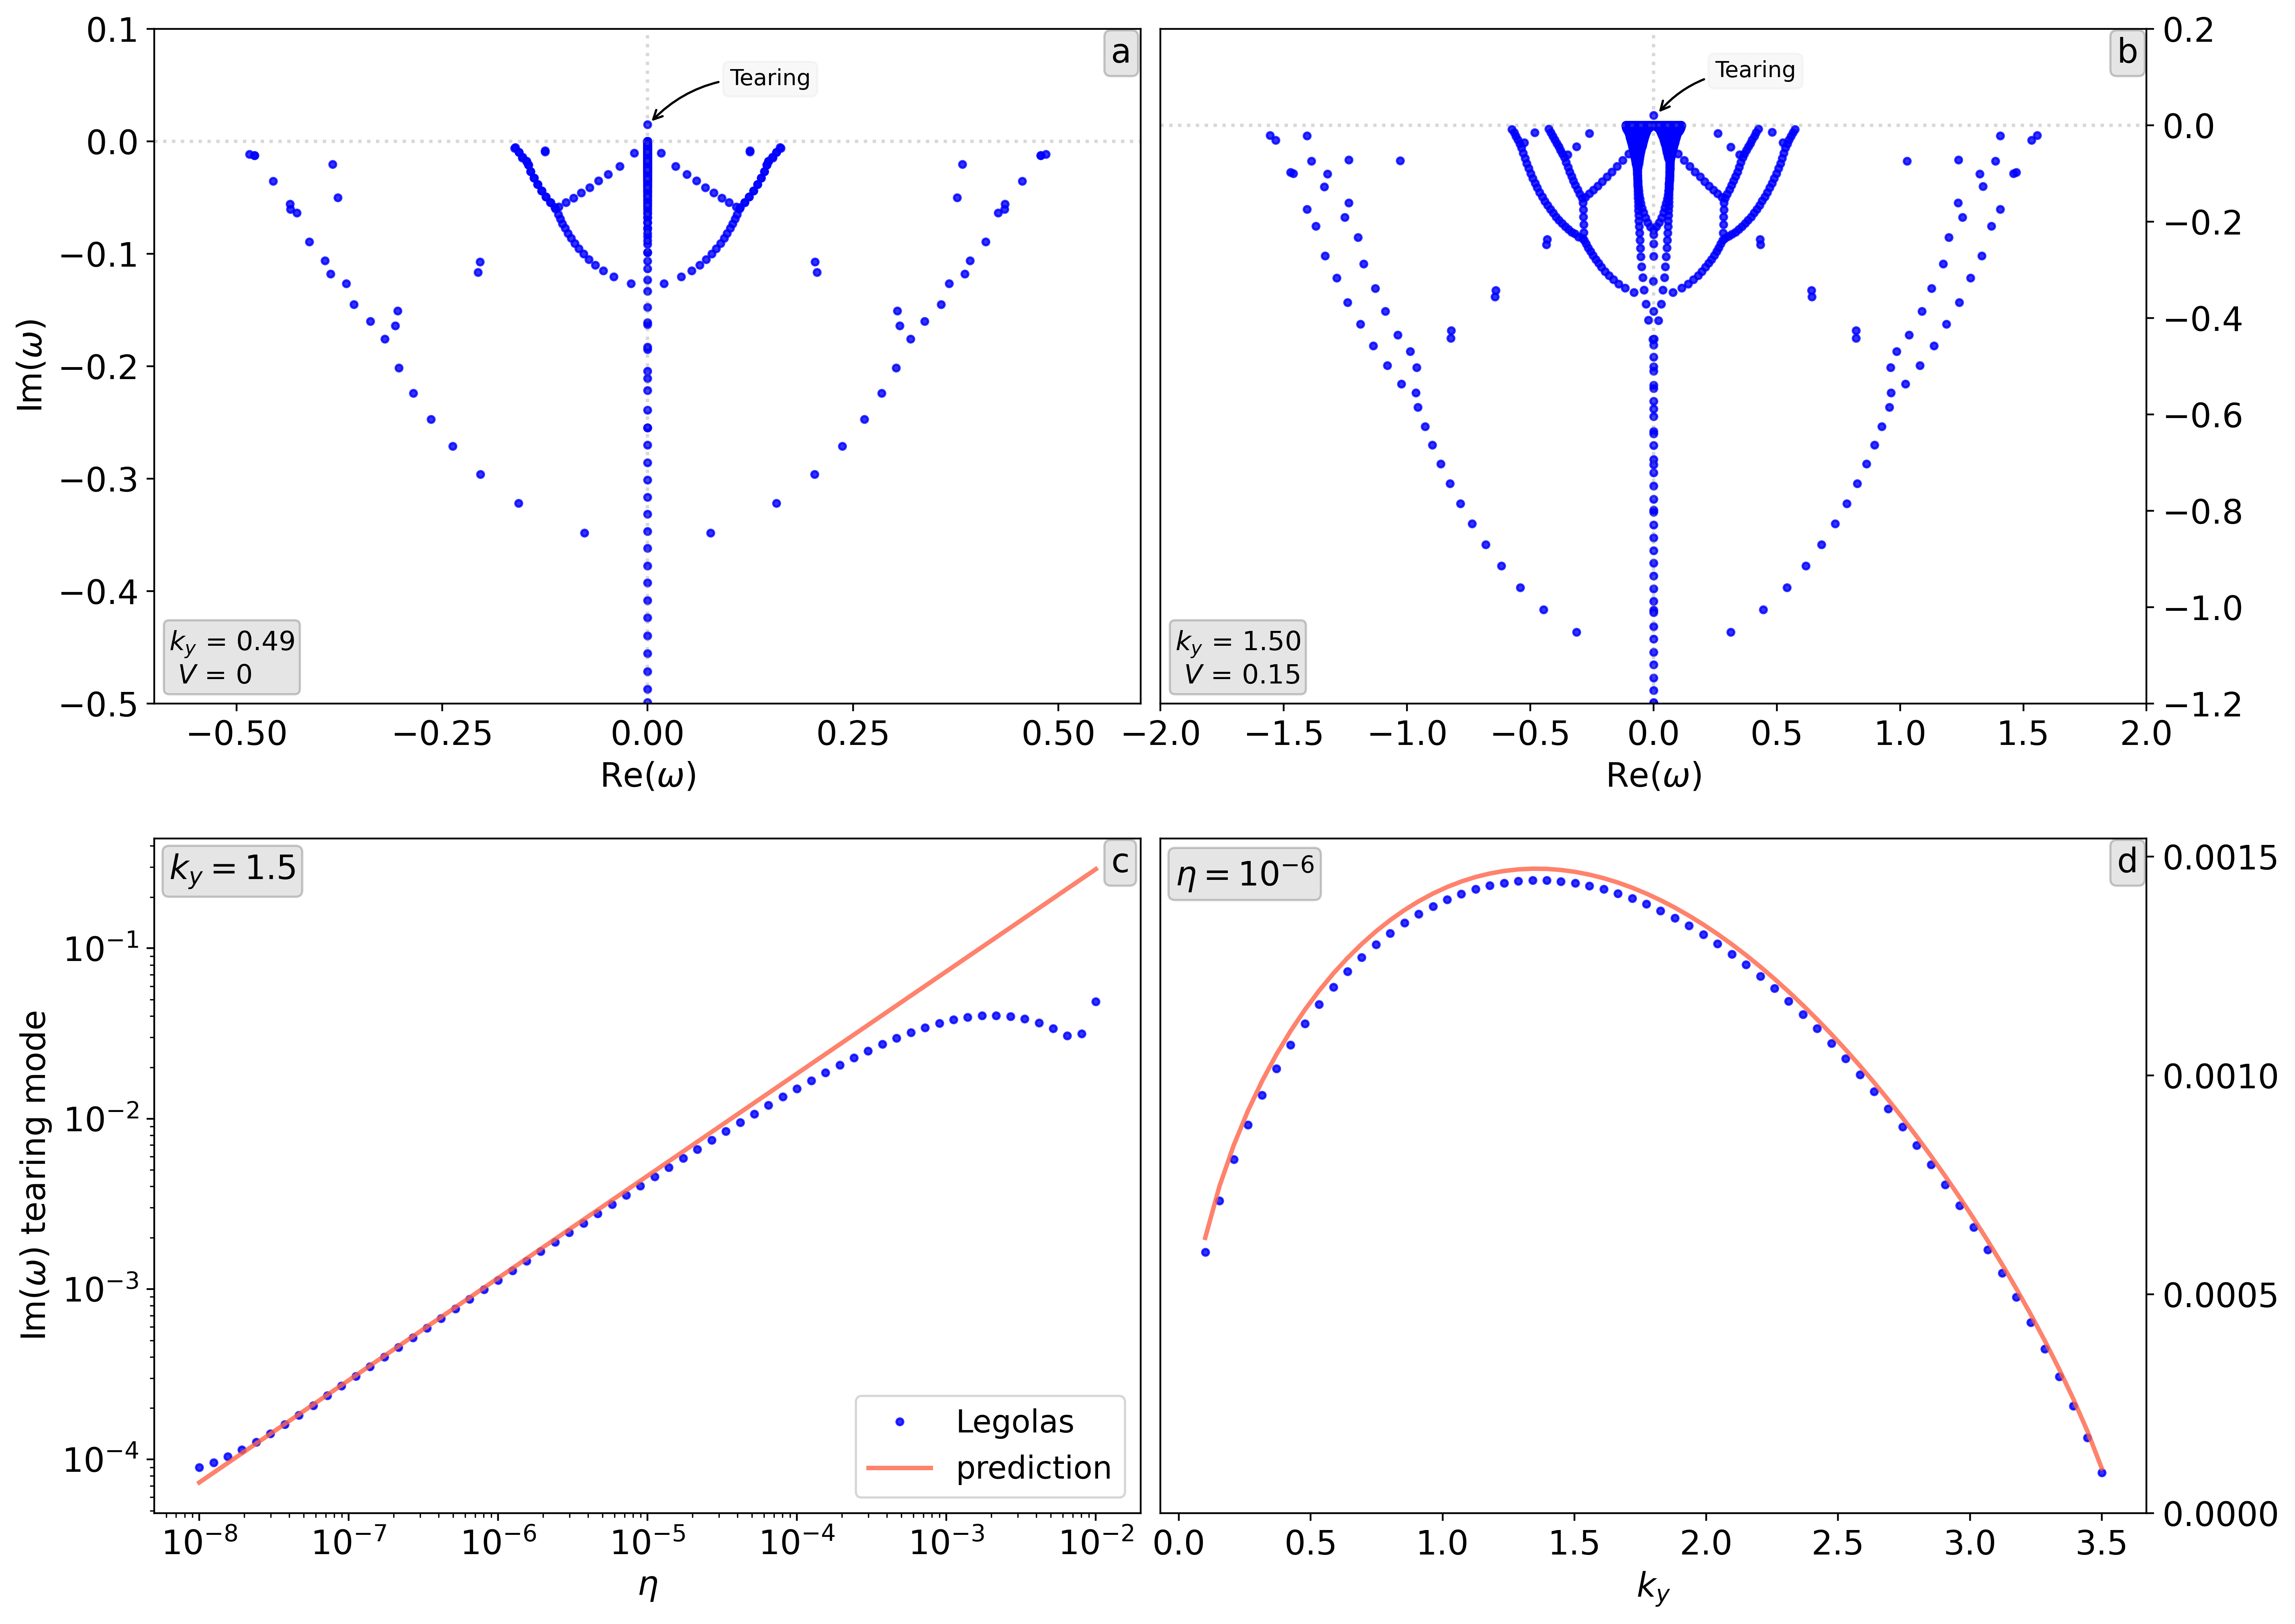
\includegraphics[width=\textwidth]{resistive_tearing.png}
  \caption{
    Resistive spectra of the equilibrium given in Equation \eqref{eq: resistive_tearing}, unstable to the tearing mode (annotated with an arrow). Panels \textbf{a} and \textbf{b} show the spectrum without and with a linear flow profile, respectively, zoomed in to reveal the complex structure of the slow and Alfv\'en modes (fast modes are not shown). Panels \textbf{c} and \textbf{d}: growth rate of the tearing mode vs. fixed $k_y$, varying $\eta$ and fixed $\eta$, varying $k_y$, respectively. Both bottom panels are cases without flow, with 64 runs of 351 gridpoints each, per panel. The red line in Panels \textbf{c} and \textbf{d} denotes the theoretical growth rate prediction given in Equation \eqref{eq: tearing_growthrate}.
  }
  \label{fig: resistive_tearing}
\end{figure}

For a thorough discussion on tearing modes, we refer to \citet{book_MHD}, where they perform a detailed analysis on the resistive MHD equations to derive an analytical expression for the growth rate of the tearing mode, given by
\begin{equation} \label{eq: tearing_growthrate}
  \begin{aligned}
    \text{Im}(\omega) &= \magneticreynolds^{-3/5}(KH)^{2/5}\left(\frac{\Delta'}{C}\right)^{4/5}\alfvenspeed / a,
    \qquad
    \text{in which} \\
    \Delta' &= -2\sqrt{H^2 - K^2}\cot\left(\frac{1}{2}\sqrt{H^2 - K^2}\right),
  \end{aligned}
\end{equation}
with $\magneticreynolds = a \alfvenspeed / \eta$ the magnetic Reynolds number, $a$ the width of the slab, and $\alfvenspeed$ the Alfv\'en velocity. The other parameters in this equation are variables introduced during the analysis, given by
\begin{equation}
  H = \alpha a,
  \qquad
  K = k_0 a,
  \qquad
  C = 2\pi\frac{\Gamma(3/4)}{\Gamma(1/2)} \approx 2.1236.
\end{equation}

Panels c and d of Figure \ref{fig: resistive_tearing} show a comparison of the tearing mode growth rate between the {\legolas} results (using the no-flow case) and Equation \eqref{eq: tearing_growthrate}. Panel c holds $k_y = 1.5$ constant but varies the resistivity, reaching Reynolds numbers of $\approx 10^8$, a feat that is nearly impossible to achieve if fully nonlinear codes would be used instead. The correspondence between the theoretical and numerical growth rates is nearly one-to-one, except for large resistivity values as the theoretical approximation starts to break down in those regimes. In Panel d we keep $\eta = 10^{-6}$ (magnetic Reynolds number of $\approx 10^6$) constant and vary $k_y$ between 0.1 and 3.5, which again yields excellent agreement between theory and numerical results. For both Panels c and d we performed 64 runs of 351 gridpoints each.



\section{Nonadiabatic, cylindrical cases}
Because {\legolas} is the first linear MHD code to simultaneously include nonadiabatic effects, resistivity, and flow, there are no known previously calculated spectra where all these physical effects are included. Nevertheless, there exist some spectra in the literature where solely nonadiabatic effects are included (and where the equilibrium is static and no resistivity is incorporated), so we will use these as a base comparison for testing the nonadiabatic terms in the implementation.

\subsection{Nonadiabatic discrete Alfv\'en waves}
The first spectrum we will look at is that of nonadiabatic discrete Alfv\'en waves, described in \citet{keppens1993}. The basic cylindrical equilibrium represents a solar loop, and nonadiabatic effects included were optically thin radiative losses and parallel thermal conduction. It was pointed out how a cluster sequence of discrete Alfv\'en waves may become unstable and could lead to disruptions or oscillatory behaviour in loops or prominences.

This particular equilibrium uses an axial current profile in a cylindrical geometry, yielding the same magnetic configuration as given in Equation \eqref{eq: tokamak_btheta} although this time with $\nu = 2$ such that a current distribution is present throughout the loop. The pressure profile can be obtained through integration of the equation for magnetostatic equilibrium \eqref{eq: force_equilibrium} without flow. As a boundary condition, we impose that the pressure vanishes at the plasma boundary $r = R$, which can be used to constrain the integration constant. Furthermore, a parabolic density profile is used, yielding an equilibrium configuration given by
\begin{equation} \label{eq: discrete_alfven_equilibrium}
  \begin{gathered}
    \rho_0 = 1 - \left(1 - d\right)\left(\frac{r}{R}\right)^2,
    \qquad
    B_{02} = \frac{1}{6}j_0 r\left(r^4 - 3r^2 + 3\right),
    \qquad
    B_{03} = 1, \\
    \begin{aligned}
      p_0 = ~&\frac{j_0^2}{720}\Bigl[
        12\left(R^{10} - r^{10}\right)
        - 75\left(R^8 - r^8\right)
        + 200\left(R^6 - r^6\right) \\ \Bigl.
        &- 270\left(R^4 - r^4\right)
        + 180\left(R^2 - r^2\right)
      \Bigr],
    \end{aligned}
  \end{gathered}
\end{equation}
in which $d = 0.2$ and $j_0 = 0.125$. The cylinder wall is taken at $R = 1$. The equilibrium temperature profile can be derived using $T_0 = p_0 / \rho_0$ and $T_0' = \left(p_0'\rho_0 - \rho_0'p_0\right)/\rho_0^2$, where the prime denotes the derivative with respect to $r$. Only conduction parallel to the magnetic field lines is taken into account,
because cross-field thermal conduction acts on too long a timescale in this case \citep{keppens1993}.

The wavenumbers $k_2 = m$ and $k_3 = k$ are taken to be 1 and 0.05, respectively. The heating term is assumed to be as such that it exactly balances out the optically thin radiative losses in the equilibrium state. We use the cooling curve introduced by \citet{rosner1978}, which represents a piecewise cooling law with predetermined coefficients. Because the inclusion of nonadiabatic effects requires us to specify unit normalisations in order to loop up the dimensional values in the cooling tables, we take reference values of 50 G for the magnetic field, $1.5 \times 10^{-15}$ g cm$^{-3}$ for the density and $10^{10}$ cm as a length scale. This automatically constrains all other normalisations through the ideal gas law, assuming a fully ionised plasma.

\begin{figure}[t]
  \centering
  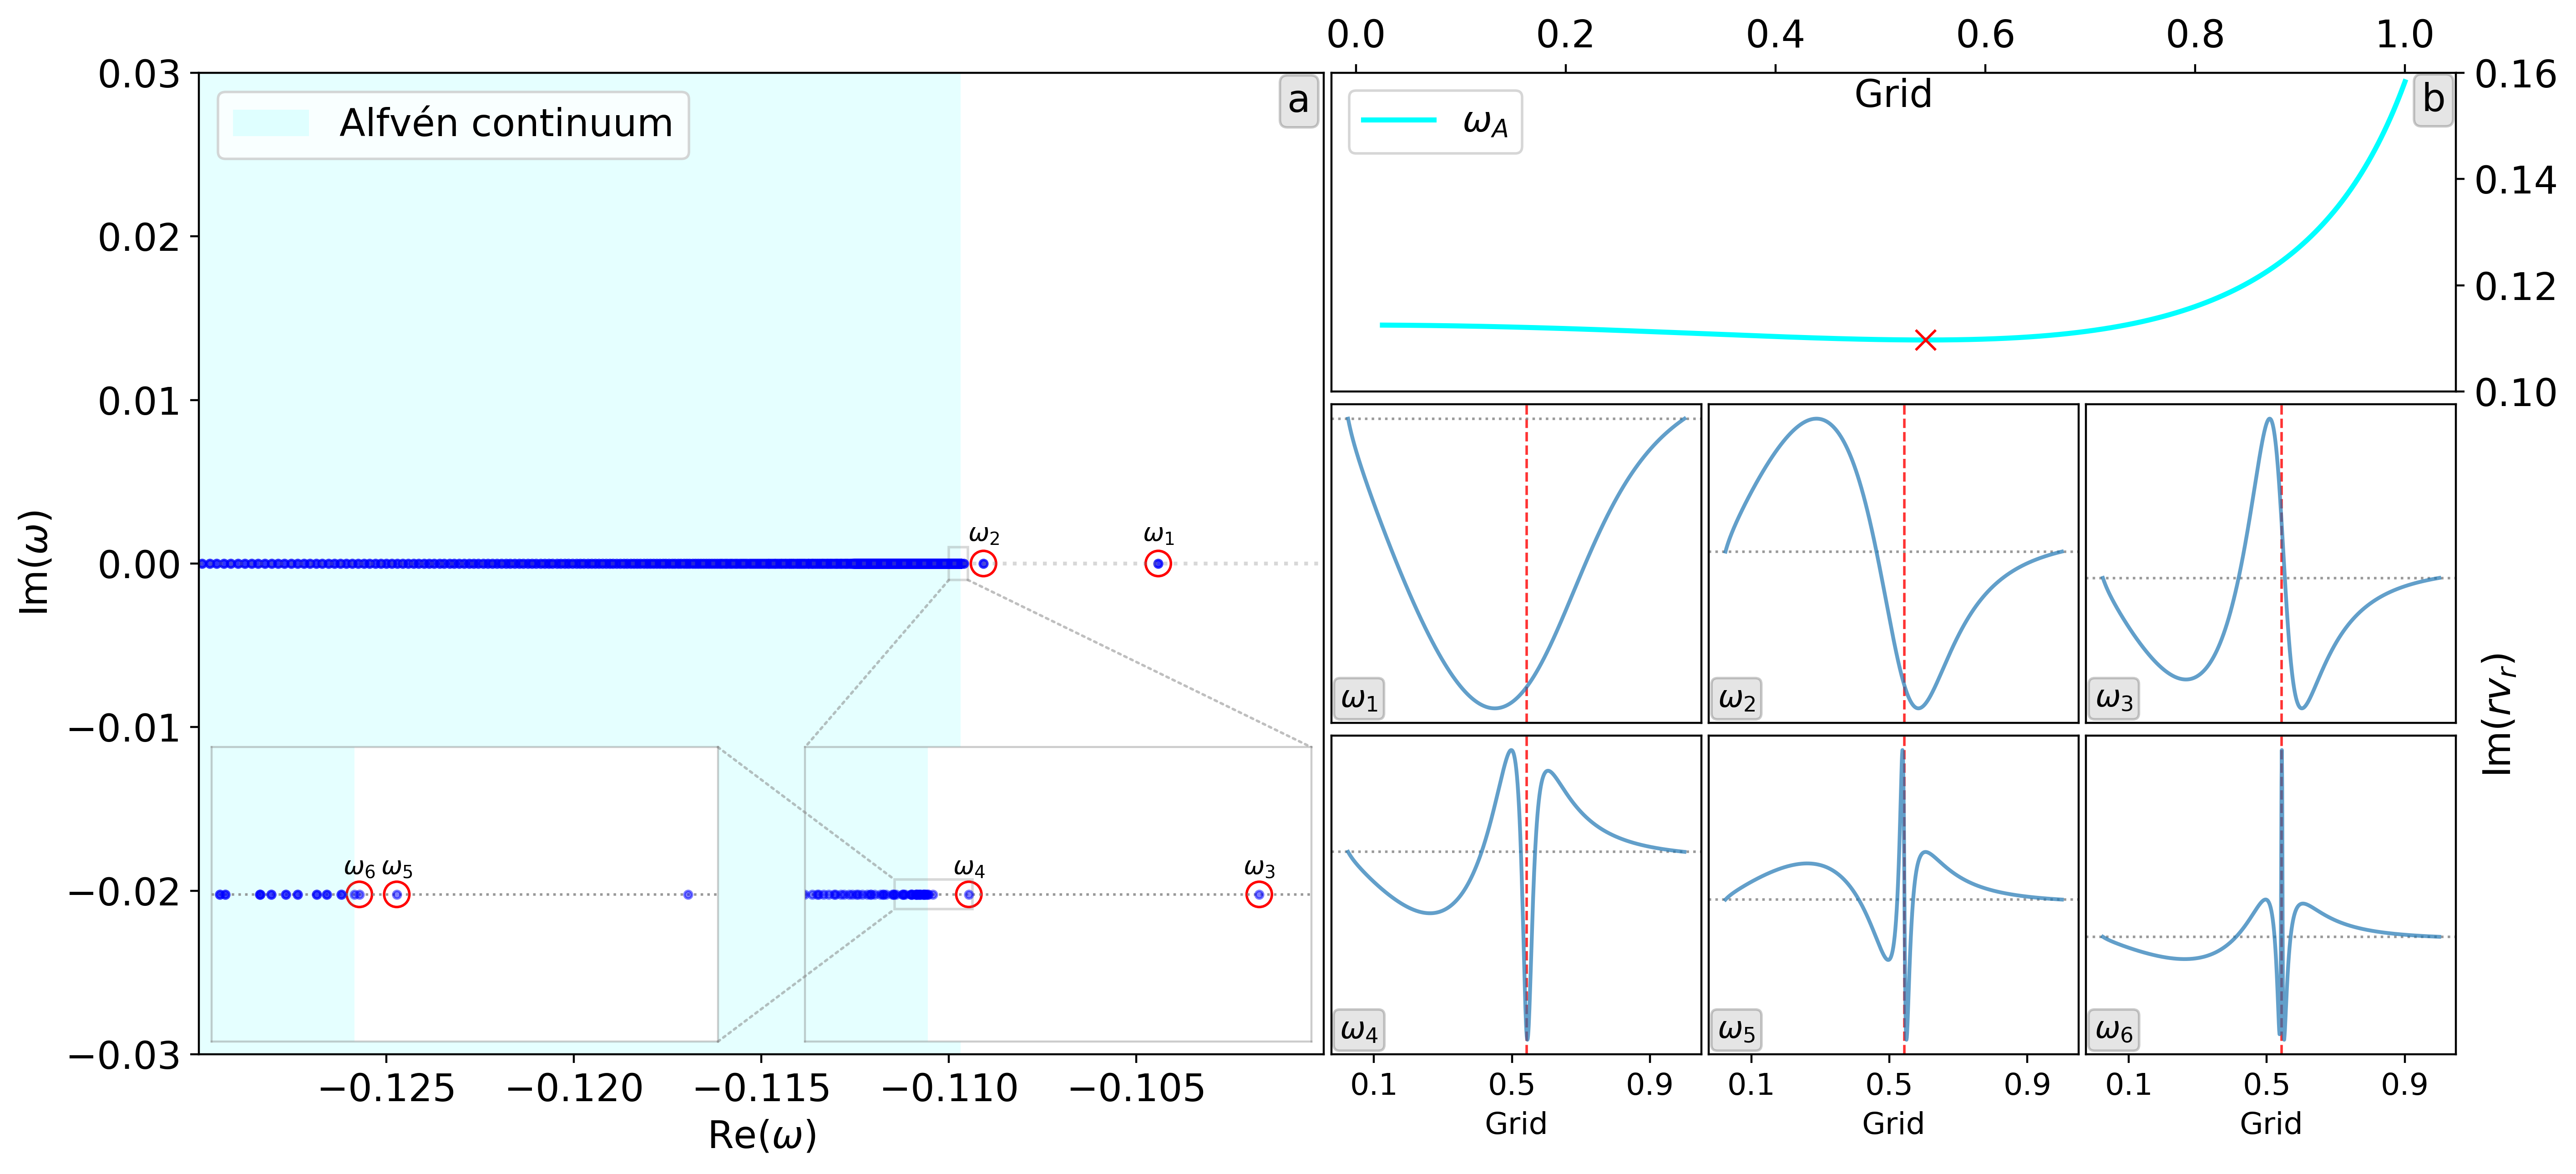
\includegraphics[width=\textwidth]{discrete_alfven.png}
  \caption{
    Panel \textbf{a}: discrete Alfv\'en spectrum; the Alfv\'en continuum is annotated in cyan. Six discrete modes were found, denoted $\omega_1$ through $\omega_6$. The insets depict zoom-ins; the regions are annotated in the figure. Panel \textbf{b} shows a plot of the Alfv\'en continuum vs. radius; the minimum is denoted by a red cross. The six panels in the bottom-right corner show the imaginary part of the $r v_r$ eigenfunctions for modes $\omega_1$ through $\omega_6$, the red dotted line represents the location of the minimum of the Alfv\'en continuum.
  }
  \label{fig: discrete_alfven}
\end{figure}

The spectrum is calculated using 501 gridpoints, Figure \ref{fig: discrete_alfven} shows the discrete Alfv\'en spectrum (Panel a) along with a plot of the Alfv\'en continuum (Panel b). In total, six discrete modes (that is, modes that fall outside of the Alfv\'en continuum) were found in contrast with the five discrete modes in the original paper by \citet{keppens1993}. The discrete modes are annotated according to their overtones, where $\omega_1$ represents the fundamental mode (FM) and $\omega_6$ the fifth overtone (OT). This last overtone does not show up for resolutions below $\sim 200$ gridpoints, which explains why it is not present in the original work. The imaginary part of the $r v_r$ eigenfunction corresponding to each of these six modes is shown in the bottom-right panels of Figure \ref{fig: discrete_alfven}, where the location of the minimum in the Alfv\'en continuum is indicated by a red dotted line. Note that the number of eigenfunction nodes increases when considering modes further in the Alfv\'en sequence: the eigenfunction corresponding to $\omega_1$ has no nodes, and $\omega_2$ through $\omega_6$ have one, two, three, four, and five nodes, respectively. Table \ref{tab: discrete_alfven} shows a detailed comparison between the discrete modes found by {\legolas} and the ones from \citet{keppens1993}.
We multiplied these latter by $\icomplex$, because they use the convention $\exp(st)$ rather than $\exp(-\icomplex \omega t)$ in the Fourier analysis (thus, $\omega = \icomplex s$).

\begin{table}[t]
	\centering
	\caption{
    Comparison of discrete Alfv\'en eigenvalues between \texttt{Legolas} and the original work by \citet{keppens1993}
  }
	\begin{tabular}{c c c}
		\hline
		\textbf{Eigenvalue}		&		\texttt{Legolas}									&				original work	\\
		\hline
      FM $\omega_1$	    &	$-0.1044166 + 1.7261\times 10^{-07}\icomplex$	&	$-0.1043688 + 1.7\times 10^{-07}\icomplex$	\\
      1st OT $\omega_2$	&	$-0.1090794 + 6.5883\times 10^{-08}\icomplex$	&	$-0.1090706 + 6.7\times 10^{-08}\icomplex$	\\
      2nd OT $\omega_3$	&	$-0.1096034 + 8.3813\times 10^{-09}\icomplex$	&	$-0.1096018 + 8.4\times 10^{-09}\icomplex$	\\
      3rd OT $\omega_4$ &	$-0.1096779 + 2.5325\times 10^{-09}\icomplex$	&	$-0.1096777 + 2.5\times 10^{-09}\icomplex$	\\
      4th OT $\omega_5$	&	$-0.1096872 + 3.7770\times 10^{-10}\icomplex$	&	$-0.1096871 + 4.0\times 10^{-10}\icomplex$	\\
      5th OT $\omega_6$	&	$-0.1096883 + 7.4336\times 10^{-11}\icomplex$	&					---
	\end{tabular}
	\label{tab: discrete_alfven}
\end{table}

In reality, the mode sequence is expected to be an infinite sequence accumulating at the local minimum in the Alfv\'en continuum, as indicated in Panel b on Figure \ref{fig: discrete_alfven}. Both the real and imaginary parts of the eigenvalues are in excellent agreement. It should be noted that when the nonadiabatic effects are omitted, the imaginary parts of these discrete modes become zero, such that they lie on the real axis, representing stable waves. The inclusion of nonadiabatic effects hence has almost no influence on their oscillation frequency and solely pushes these modes into the unstable part of the imaginary plane. In \citet{keppens1993}, it was pointed out how these discrete Alfv\'en mode sequences can be studied by means of a WKB analysis. However, this only correctly predicted the damped or overstable nature of the higher-order modes: to determine whether the most global modes of the sequence are overstable or damped requires a full numerical calculation, now possible with a tool like {\legolas}.


\subsection{Magnetothermal instabilities}
As a final test, we look at magnetothermal instabilities, originally depicted in \citet{vanderlinden1992}. The geometry is cylindrical with $r \in [0, 1]$ and an isothermal equilibrium profile given by
\begin{equation} \label{eq: magnetothermal_equilibrium}
  \begin{gathered}
    T_0 = 1,
    \qquad
    B_{02} = \frac{r}{1 + r^2},
    \qquad
    B_{03} = 0,
    \qquad
    p_0 = \frac{1}{2\left(1 + r^2\right)^2},
    \qquad
    \rho_0 = \frac{p_0}{T_0},
  \end{gathered}
\end{equation}
with $k_2 = m = 0$ and $k_3 = k = 1$. There is no $B_{0z}$, such that this configuration actually represents a z-pinch (which is very unstable), and we are looking at axisymmetric (sausage) $m = 0$ modes here. Field-aligned thermal conduction is included, cross-field thermal conduction is omitted. Optically thin radiative losses are accounted for, and we use the same cooling curve and heating assumptions as for the nonadiabatic discrete Alfv\'en waves in the previous subsection. Reference values are taken to be $2.6$ MK for the temperature, 10 G for the magnetic field and $10^8$ cm for the length scale. As before, this automatically constrains all other normalisations as well. There parameters are representative for solar coronal loops and arcades.

Both the Alfv\'en and slow continua collapse into marginal (zero) frequency. However, including finite parallel thermal conduction and radiative losses introduces the thermal continuum. Together with the marginal slow-Alfv\'en frequencies, this organises the modes such that thermal instabilities merge with magnetic modes, introducing magnetothermal branches. Figure \ref{fig: magnetothermal} shows the MHD spectrum for 1001 gridpoints in the region of the magnetothermal branches, where the bottom-right Panel c zooms in further near the origin. The modes denoted by $I_{+1}$ and $T_1$ represent fundamental magnetic and thermal modes, respectively, meaning they are not coalesced.
The overtones of these modes on the other hand are coalesced; these are denoted by $\left(I_{+2}, T_2\right)^-$ and $\left(I_{+15}, T_{15}\right)^-$ for the 1st and 14th overtones, respectively. The minus sign in superscript means they are located on the negative side of the real axis. There are corresponding modes on the positive part of the real axis, as without flow, we maintain left-right symmetry of the spectrum. The first 14 overtones are in excellent agreement with those described in \citet{vanderlinden1992} and are encircled in red on Panel a. However, the original work only displays solutions up to the 14th overtone. The resolution used here is much higher than the originally published results, allowing us to probe the region near the origin as well. Panel c zooms in near the origin, denoted by the dashed rectangle in Panel a, revealing a complex mixture of different branches and scattered modes. It seems that the original magnetothermal branches split, and a dense region covered with many magnetothermal modes appears. The (analytically known) thermal continuum is annotated in green on the figure, and is represented by a dense, continuous range of discrete eigenvalues on the imaginary axis. Because this is the first time that such high resolutions are possible for computing the magnetothermal modes, it is left to future work to clarify how the MHD spectrum allows for such complex mode interactions, revealing the possible presence of areas covered by modes in the complex eigenfrequency plane.

\begin{figure}[t]
  \centering
  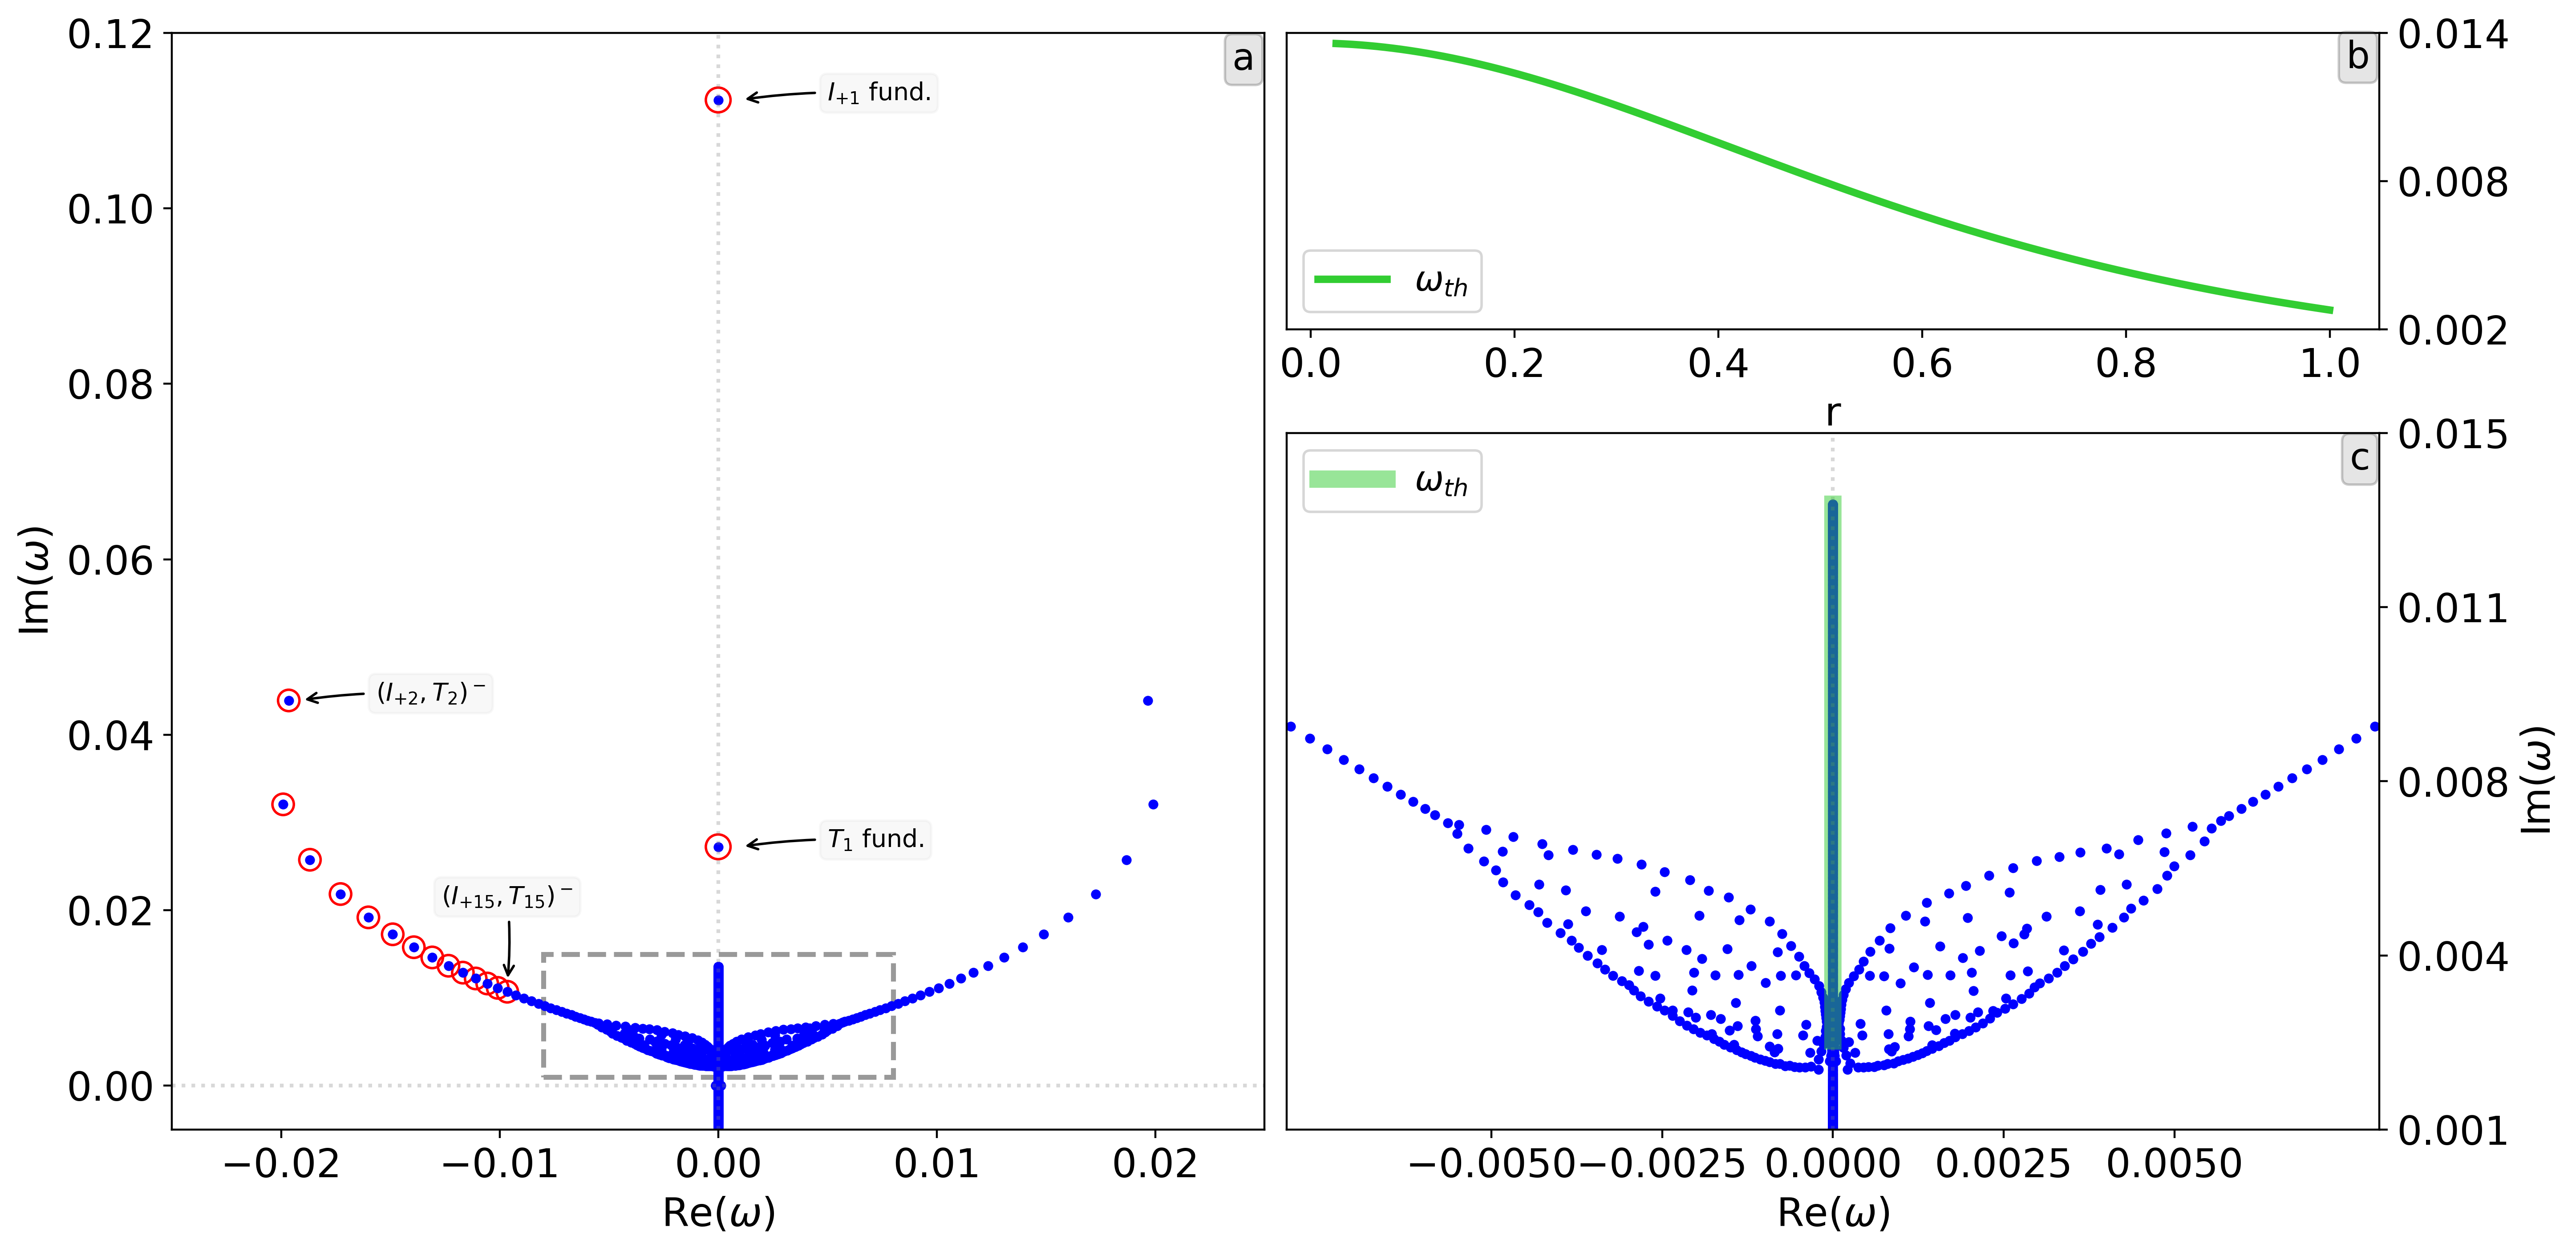
\includegraphics[width=\textwidth]{magnetothermal.png}
  \caption{
    Magnetothermal instabilities for $m = 0$ and $k = 1$. The fundamental modes and 14 overtones discussed in the original work are encircled by red and denoted in the left Panel \textbf{a}. Panel \textbf{b} shows the thermal continuum as a function of radius. Panel \textbf{c} zooms into the region denoted by dashed lines in Panel \textbf{a}, revealing various other modes forming intricate structures.
  }
  \label{fig: magnetothermal}
\end{figure}

\section{Convergence} \label{sec: convergence}
As is clear from all cases discussed in this Chapter, increasing the resolution can have a major influence on the spectrum, depending on whether or not all modes are sufficiently resolved. Generally speaking, the further one goes in a specific sequence, that is, looking at larger mode numbers that represent overtones having more and more nodes in their eigenfunctions, the higher the resolution that is required in order to resolve the mode completely. For eigenfunctions, it is usually immediately clear if a mode is resolved or not, because higher mode numbers translate into more oscillations in the eigenfunction. Hence, once the number of oscillations approaches the amount of gridpoints, the eigenfunction will no longer be resolved.

For the eigenfrequencies it is not a priori clear when a specific $\omega$ is resolved. One way to constrain an eigenvalue is to do multiple runs, each time increasing the resolution. Once an eigenvalue no longer shifts in the complex plane, it can be considered resolved, and increasing the resolution even further will not have much effect on its value. Now, the question of how many gridpoints are typically needed to be able to speak of a ``resolved'' spectrum naturally arises. This will strongly depend on the type of equilibrium considered: for smooth equilibria without sharp transitions, one can get away with a few dozen gridpoints and already reach an acceptable accuracy for most modes. However, in the case of equilibria with large gradients, or even with localised discontinuities (interfaces), one has to make sure that a sufficient number of gridpoints are taken in order to sufficiently resolve that jump.

Furthermore, the amount of eigenvalues in the spectrum increases with resolution, because there are as many eigenfrequencies as the dimension of the matrices (which is 16 times the number of gridpoints, at least for the 8 MHD equations). It is therefore entirely possible that one starts probing parts of the spectrum that were initially not visible at lower resolutions, simply because there were no eigenvalues in that region for that amount of gridpoints. An example is given here, where we look back at the Kelvin-Helmholtz equilibrium discussed in Section \ref{ss: kh_cd_instabilities}. Figure \ref{fig: convergence} shows this equilibrium for the exact same values as employed earlier, but every panel shows the spectrum for a different resolution, with the amount of gridpoints given in the top-left corner. The first three panels start out at low resolution, increasing from 26 to 76 gridpoints. Three modes are annotated on the figure, corresponding to the KH and CD modes discussed earlier. These modes are already decently resolved even at the lowest resolutions and can be considered completely resolved at around 100 gridpoints. However, the region near the horizontal axis is another matter entirely. At low resolutions (first three panels), we see that most of the modes here are almost randomly scattered in the complex plane. At around 100 gridpoints, they start lining up and form a more intricate ``elliptic'' pattern. This is the point where the original paper by \citet{baty2002} stopped, because back then it was not really feasible to run these codes at higher resolutions, and they were only interested in the most unstable KH and CD modes that were resolved, and that determined the early evolution of a full nonlinear MHD simulation that they performed.

\begin{figure}[t]
  \centering
  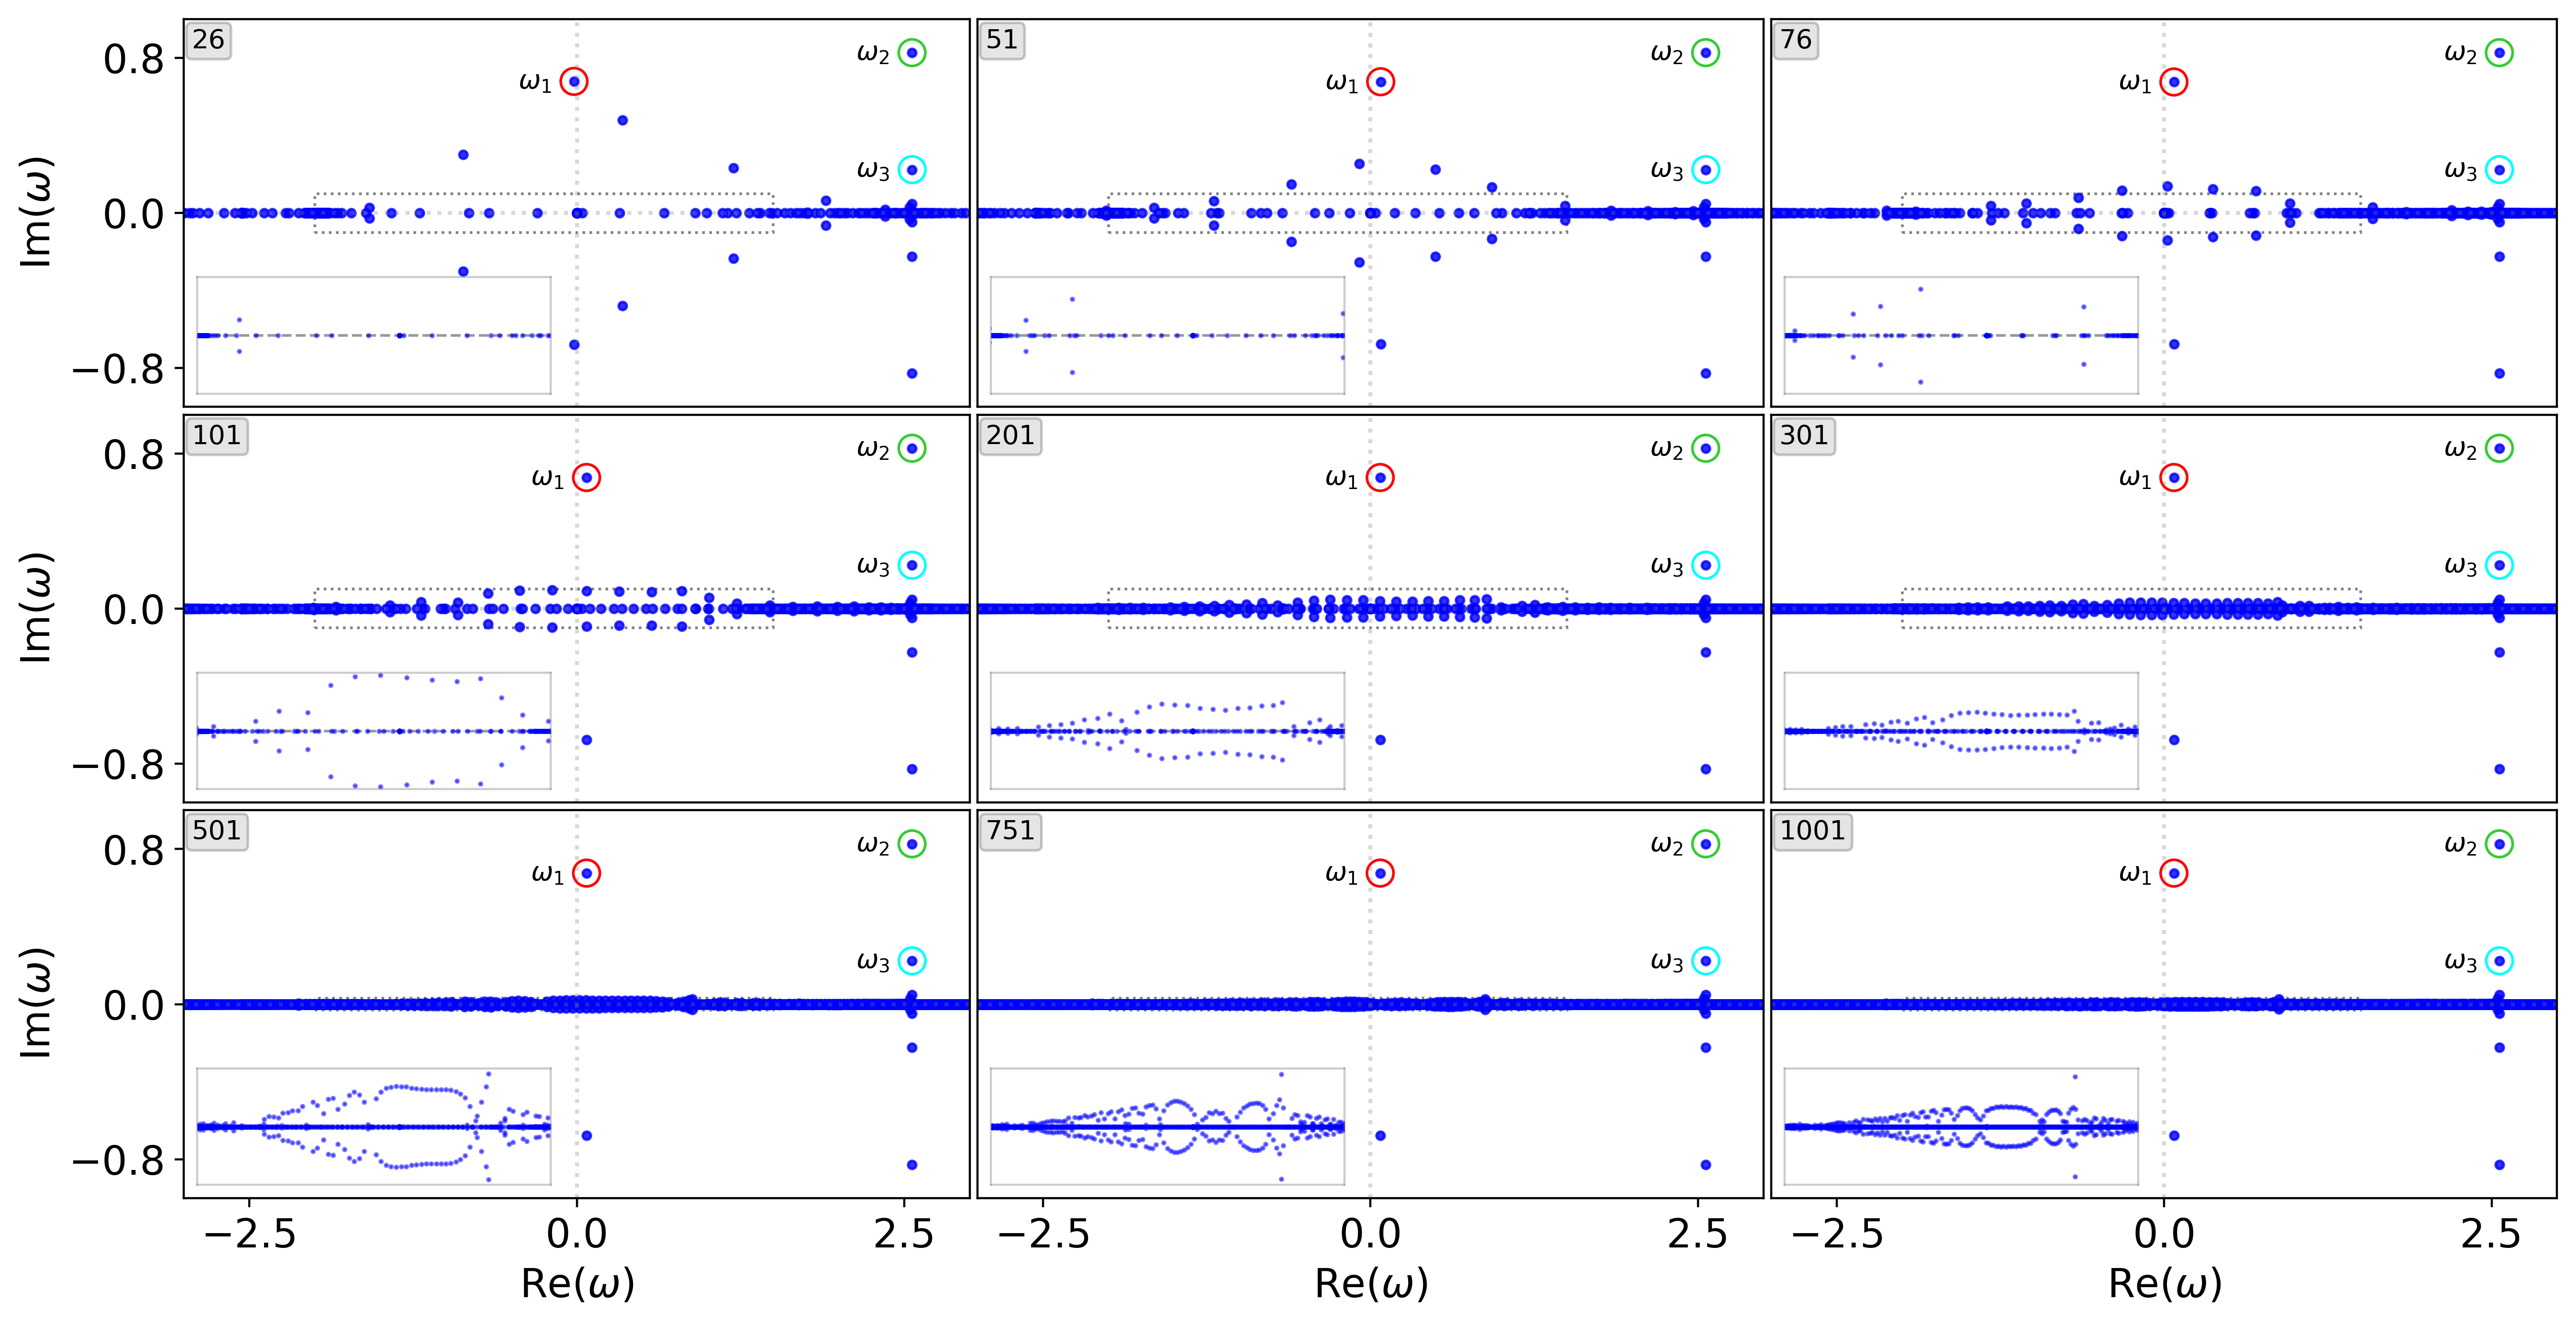
\includegraphics[width=\textwidth]{convergence.png}
  \caption{
    Spectrum of the Kelvin-Helmholtz and current-driven equilibrium as shown in Figure \ref{fig: kh_cd}, using the same parameters as in Section \ref{ss: kh_cd_instabilities}, at various resolutions (indicated on the top-left of each panel). The inset on the top two rows of panels zooms near the horizontal axis, for vertical axis values between $-0.1$ and $0.1$. The insets on the bottom row of panels have slightly different vertical bounds, from $-0.03$ to $0.03$.
  }
  \label{fig: convergence}
\end{figure}

When the resolution is increased even further, we see that the near-axis modes shift even closer to the real eigenfrequency axis, and as visible on the insets of each panel, these modes start to form intriguing patterns at high resolutions. The amount of ``scattered'' modes decreases considerably, and a helix-like structure is formed at very high resolutions (1001 gridpoints, lower-right panel). These complex and almost geometric patterns may arise in various different equilibria as well and call for extensive research in this topic. A complementary means to identify which modes are actually resolved is to exploit the spectral web; see \citet{goedbloed2018_web1, goedbloed2018_web2} and \citet[Ch. 12--13]{book_MHD}, who locate eigenmodes on specific curves and their intersections. These curves relate to the two self-adjoint operators at play in stationary, adiabatic MHD. Only a combined approach using high-resolution {\legolas} runs, modern linear algebra solvers, and physical insight in MHD spectral theory will in time reveal the true importance of these modes.

Based on the conclusions drawn here, it is clear that the resolution required depends on the part of the spectrum that is to be investigated. For isolated modes, about 100 gridpoints is usually more than sufficient to resolve most of them, although this also depends on the equilibrium under consideration. For large-scale surveys of the spectrum, large resolutions should be employed in order to reveal possible regions of interest.


\section{The Legolas testing framework} \label{ss: legolas_testing}
As with any newly developed numerical code, a proper and extensive testing framework is (supposed to be) an integral part of the development process. Every step of the way a developer should make sure that newly added code actually works and does what it is supposed to do; at the same time proper care must be taken to make sure that previously working code does not get broken due to newly added changes or features. For small codebases this can be done through a quick manual check, but this rapidly becomes cumbersome and even impossible for larger projects. {\legolas} falls in this second category, where it becomes unfeasible to manually check every single equilibrium against known results for every change made to the code. Ideally then, this process should happen automatically, which is where the testing framework comes in. Before simply writing ``tests'' however, one should carefully think about \emph{what} should be tested and \emph{how} tests are written. A test should be robust, meaning that it should be easily ported over to other platforms; and at the same time be as sensitive as possible to any breaking changes, meaning tests should fail as soon as inconsistencies are introduced. Additionally, tests should be able to run in a reasonably small amount of time. Care should also be taken to make the tests as independent of the code itself as possible: a scenario where the tests themselves have to be continuously modified following minor changes in the code base should be avoided at all cost.

The {\legolas} testing framework is split up in three main parts: \emph{unit tests}, which test individual code subroutines completely independently of one another; \emph{regression tests}, which test spectra and eigenfunctions against known results; and \emph{Pylbo tests}, which test the data reading routines and post-processing logic. These latter tests are linked to the post-processing framework \textsf{Pylbo}, which was developed along with {\legolas}, but we will not go into detail on those here.

\subsubsection{Unit tests}
The backbone of the testing framework is the unit tests, which are specifically designed to ensure that a particular part of the code (a ``unit'') works as intended. Usually one or more unit tests target a single subroutine, call it with a particular set of parameters that are chosen in such a way that the expected result is known, and the subroutine's output is compared against this known result. In most cases one subroutine is accompanied by multiple tests, where every single test handles one specific case. This also includes ``edge cases'', that is, sets of parameters that may trigger some special behaviour in a subroutine. For example, consider a subroutine with as sole purpose to find a specific value in an array and return its index. This may have a couple of tests: one or two are checking that returned values are actually the ones that we expect; at least one test is checking that the routine fails to return anything if the value is not found in the array; and at least one test checks that edge cases are properly handled, such as multiple elements with the same value in the array or accessing the array out-of-bounds.

The main advantage of unit tests is that they are independent of other routines, hence bugs that are introduced can be quickly narrowed down based on the failing units -- provided these properly cover all parts of the source code. Confidence in newly developed routines will increase considerably if tests pass, and potential bugs can be caught early on. {\legolas} makes use of the open-source pFUnit framework, originally created by developers from NASA and specifically designed for unit testing of (MPI-parallel) software written in Fortran. Figure \ref{fig: unit_test} shows an example of a unit test, where the \textsf{{@}test} decorator above the subroutine marks this as a test. In this particular case an elemental function \textsf{is\_NaN} is tested, which checks a given double-precision value or array for NaN (Not a Number) values. The \textsf{{@}assertFalse} and \textsf{{@}assertTrue} statements in turn check that the function returns what is expected, and the test will fail if one or more conditions are not true when they should be, or vice-versa.

\begin{figure}[t]
  \centering
  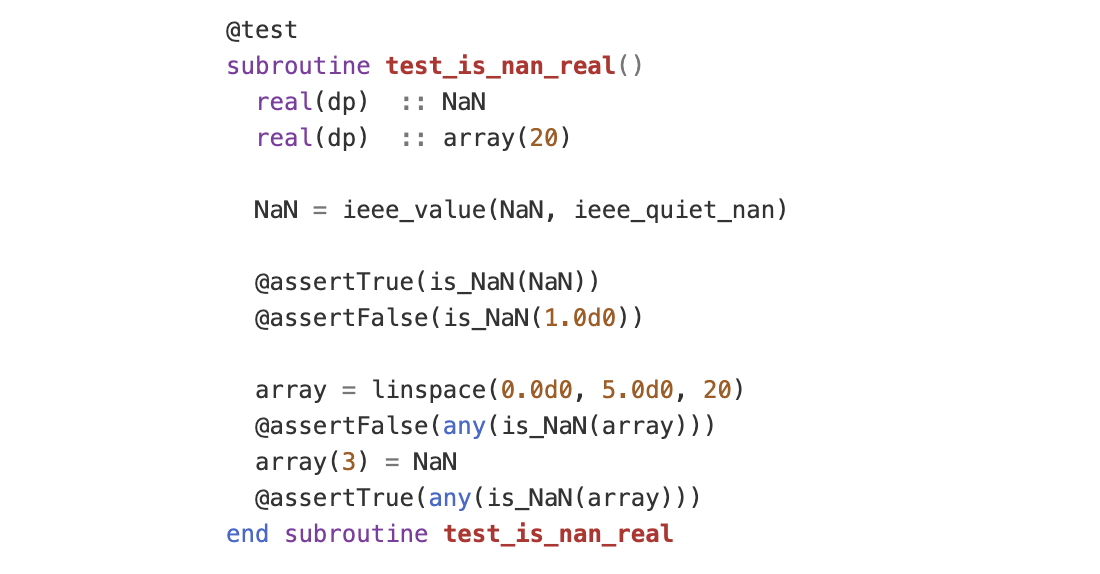
\includegraphics[width=0.80\textwidth]{unit_testing.png}
  \caption{
    Example of a {\legolas} unit test, using the pFUnit framework.
  }
  \label{fig: unit_test}
\end{figure}

\subsubsection{Regression tests}
The most important part of the testing framework are the regression tests. While unit tests are a necessary requirement to check individual subroutines and functions, they do not guarantee that the solutions to the eigenvalue problem are still the same after a code change. Additionally, it is quite difficult for the unit tests to cover everything; the matrix elements for example are quite difficult to test individually, and for those we have to resort to other approaches. The idea behind the regression tests is quite straightforward: compare the solutions, that is, both the eigenvalues and eigenfunctions, to previously (known) solutions for the implemented equilibria. However, there are a few caveats that must be addressed first: the main problem here is that we want to compare \emph{numerically calculated eigenvalues} on large scales, meaning that the actual testing is not as simple as ``just comparing solutions''. Suppose we have calculated eigenvalues for a certain equilibrium, and we know that these are correct based on a comparison with theoretically derived solutions. We call these results the ``base'' answers and store them in an array $S_\text{base}$. After a while the tests are being rerun after a change in the code base, and the solutions to the exact same problem are calculated again using the ``new'' code. Say these results are stored in an array $S_\text{test}$, resulting in the following six solutions

\begin{equation}
  \begin{aligned}
    S_\text{base} &=
      &&1.5
      &&-2 + 3\icomplex
      &&\quad 0
      &&\qquad\quad 2\icomplex
      &&-0.5\icomplex
      &&-1 - 1.0\text{e}^{-8}\icomplex \\
    S_\text{test} &=
      &&1.5
      &&-2 + 3\icomplex
      &&1\text{e}^{-15}
      &&-1\text{e}^{-16} + 2\icomplex
      &&-0.5\icomplex
      &&-1 - 1.1\text{e}^{-8}\icomplex
  \end{aligned}
\end{equation}

Note that these tests may run on different machines running different operating systems; additionally different compilers or library versions (such as for BLAS and LAPACK) may be used, which in turn can give slightly varying solutions. One can naively start comparing these two arrays, but will quickly run into a couple of problems. First of all, there is no strict guarantee that the \emph{ordering} of the solutions is the same, meaning the array needs to be sorted first. If we decide to sort based on the real part first, followed by the complex part, then the test for the above two arrays will immediately fail. While the third and fourth item of $S_\text{base}$ are saved as 0 and $2\icomplex$, the third and fourth item of $S_\text{test}$ have \emph{numerically zero} parts, with a very small but finite (up to machine precision) value deviating from zero. When $S_\text{base}$ gets sorted, 0 will be placed before $2\icomplex$, while for $S_\text{test}$ the $1\text{e}^{-15}$ solution will be sorted \emph{after} $-1\text{e}^{-16} + 2\icomplex$; resulting in the wrong eigenvalues being compared with one another.

One could argue here that a solution would be to force small values deviating from zero to actually be zero. This immediately gives rise to another problem: what is ``small''? Note that we are not comparing fixed arrays with machine precision variations, we are comparing numerical solutions to an eigenvalue problem where machine precision variations may give rise to solutions that actually differ more than machine precision. Furthermore the tolerance is eigenvalue-dependent: imagine a difference between base and test results of $10^{-6}$; for an eigenvalue of 2.5 this is perfectly fine, and the test should pass. However, for an eigenvalue of $3 \times 10^{-6}$ this is clearly too much, and the test should fail. These situations are fairly common, as the complexity of MHD spectra may result in solutions that differ many orders of magnitude within a single spectrum.

We could try opting for a percentage-based comparison, or absolute versus relative differences, but then again, \emph{how do we specify the tolerance}? As we just mentioned this is problem-specific, and we do not want our tolerances to be too robust since then we might miss out on important changes in the spectrum. No matter the solution employed here -- be it checking for absolute values, relative differences, separate real/imaginary parts, etc. -- we will eventually always run into a special case in which our strategy will fail due to numerical variations in calculating the eigenvalues.

Clearly, directly comparing eigenvalues to each other is not the right approach. A much better strategy is to compare the \emph{locations} in the spectral plane, where we actually plot the spectrum and highlight position shifts in the eigenvalues. This will eliminate much of our numerical issues, and we can ensure that the way the spectrum is drawn happens in exactly the same manner across different platforms. In {\legolas}, the regression tests are handled as follows
\begin{enumerate}
  \item[i)] For a given test, load the file with stored results and plot (at least one) spectrum with given limits for the real and imaginary axes, save the image(s) as baseline.
  \item[ii)] Execute the corresponding test, plot the spectrum for the obtained results with the exact same settings used to create the baseline figure. Save the image(s).
  \item[iii)] Load both the test and baseline images, remove everything (background, axes, axes ticks etc.) except the eigenvalues. Calculate the Root-Mean-Squared (RMS) pixel difference between the two images as
  \begin{equation}
    \text{RMS} = \sqrt{\text{mean}\Bigl(\left(\text{expected} - \text{actual}\right)^2\Bigr)}.
  \end{equation}
  \item[iv)] Set a strict RMS tolerance, check whether the calculated RMS lies within this tolerance. If this is not the case fail the test, otherwise flag it as a pass.
\end{enumerate}
The above testing strategy has proven to be very successful, both in terms of robustness and reliability. An example is given in Figure \ref{fig: regression_test}, where the Suydam cluster spectrum from Equation \eqref{eq: suydam_equilibrium} is shown both as a baseline and for a small shift in parameters. At first sight both spectra are similar, however the RMS shows clear difference between the spectra, failing the test. The main advantage of this approach is that we can generate as much image comparisons as required: for one equilibrium we typically calculate the solutions to the eigenvalue problem once, and then generate baseline images for different parts of the spectrum. This allows for spectrum testing at different scales, where we can zoom in and focus on different regions for more accurate testing.

\begin{figure}[t]
  \centering
  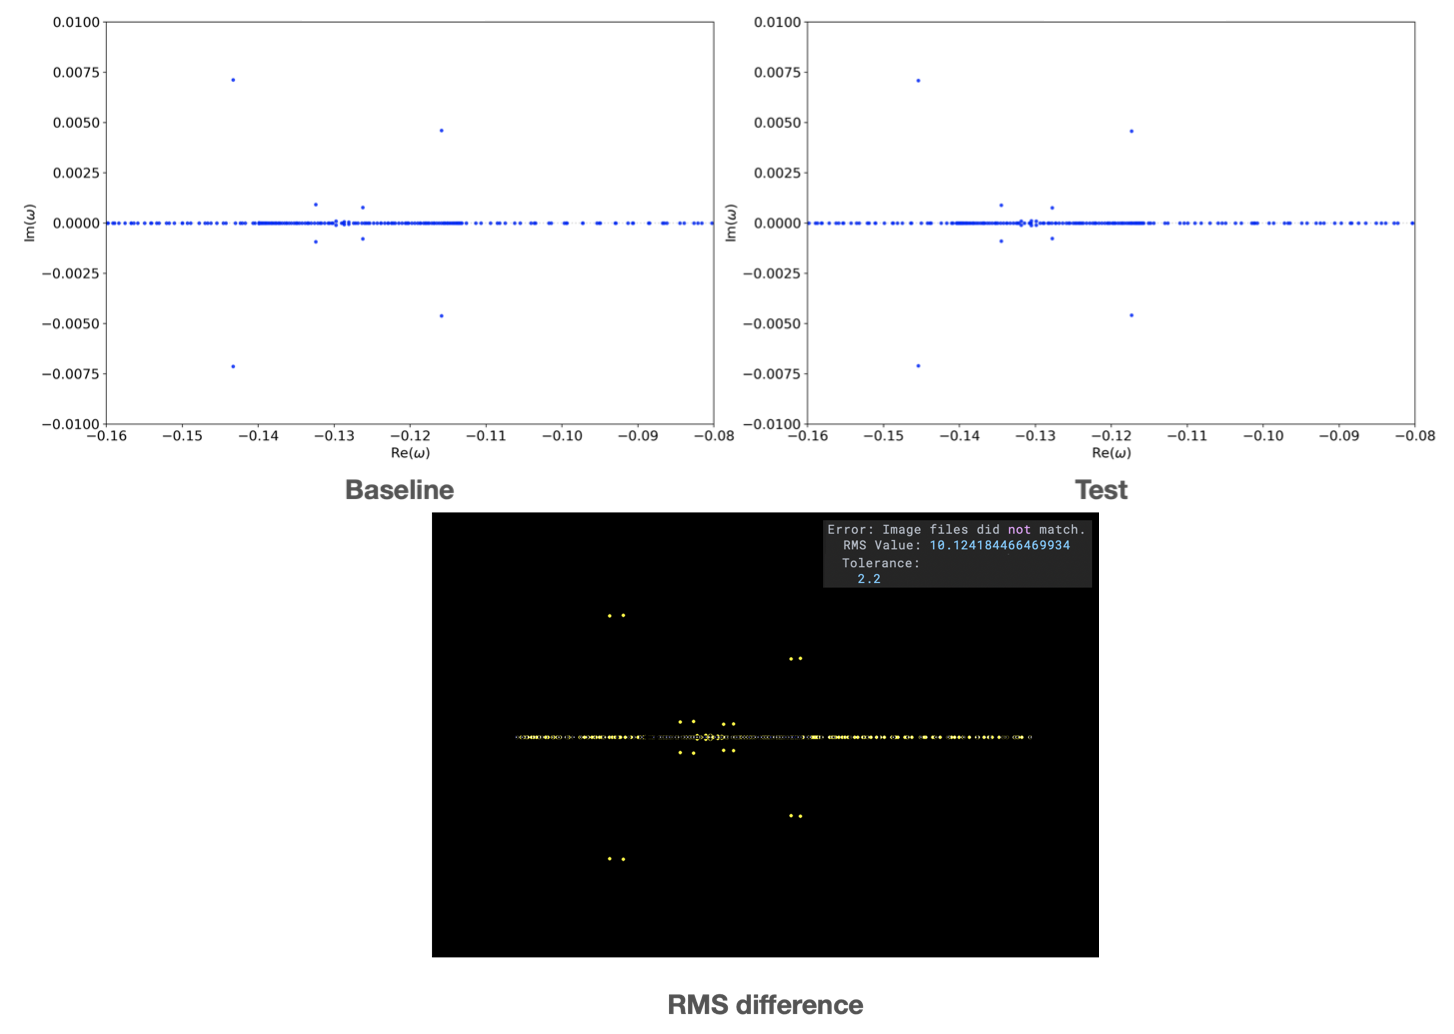
\includegraphics[width=\textwidth]{regression_testing.png}
  \caption{
    A typical example of a {\legolas} regression test, here for the Suydam cluster equilibrium. The top two images indicate the baseline spectrum (stored answer) and test spectrum (calculated answer), respectively. The bottom image shows the Root-Mean-Squared pixel difference between the top two images, the calculated RMS ($\approx 10$) is much larger than the tolerance RMS ($= 2.2$).
  }
  \label{fig: regression_test}
\end{figure}

\section{Discussion} \label{ss: legolas_discussion}
In the previous Chapter we introduced the novel finite element code {\legolas}, meant to tackle the complete MHD spectrum including all kinds of physical effects, and able to look at various realistic equilibrium configurations. The general formalism introduced can handle both Cartesian and cylindrical geometries, and with the various physics included in the formalism this makes {\legolas} the first MHD spectral code to combine the effects of flow, resistivity, gravity, radiative cooling, and anisotropic thermal conduction, even supplemented with selfgravity, viscosity or Hall MHD. This opens the door to novel, in-depth studies of the complete MHD spectrum, which was up to now impossible with existing numerical tools.

In this Chapter we tested {\legolas} against various previously established results from the literature, looking at the comparison to analytical results as well as to spectra previously obtained by similar numerical codes. Correspondence with existing results is in most cases one to one, greatly increasing the confidence in the new tool. Some cases were run in (much) higher resolutions than their original counterparts, revealing interesting features and additional structure in the spectra. As can be seen when looking at the instabilities of a cylindrical magnetised jet flow in Section \ref{ss: kh_cd_instabilities}, the outer KH and CD modes are in perfect correspondence with the original results. However, the high resolution revealed complex structures that were not probed before, and this becomes even clearer in the convergence study of Section \ref{sec: convergence}, where we used the same setup but increased the resolution even further. It is clear the the spectrum evolves drastically at higher resolutions, when more and more modes are becoming properly resolved. Because a complete knowledge of the MHD spectrum of flowing equilibria is lacking, tools like {\legolas} and careful converged studies will be essential to unravel the role as of yet unresolved spectral structure.

We speculate that these spectral structures have a physical meaning, which can be corroborated in adiabatic flowing cases with a complementary spectral web approach. Our speculation extends to cases that address MHD modes in cylindrical accretion disks \citep{keppens2002}, where it is becoming clear that many more modes than the celebrated MRI enrich the spectral structure. This has been confirmed in recent work by \citet{goedbloed2022_sari} where the SARI modes were found to be of essential importance in instability studies of accretion disks around black holes. These modes appear to open up completely new pathways to turbulence, highlighting the importance of a linear eigenmode perspective for dynamical systems even further.

Also in nonadiabatic cases interesting things were encountered: the outer modes of the magnetothermal sequence are again in perfect correspondence with modes found in the original work; however, near the origin -- a region that has never been investigated until now -- there are indications of a splitting of the magnetothermal sequence in its thermal and magnetic counterparts with various modes scattered in between. An in-depth study of magnetothermal instabilities is called for, a topic of research that essentially stopped progressing for the last two decades. Now that high-resolution MHD simulations start to reveal the complexity of thermal-instability-driven evolutions, a revival of this topic is urgently needed.

All of the above is clear indication that a thorough investigation of the entire spectrum is needed in order to yield new insights in (M)HD instabilities. For solar applications alone, the effect of thermal conduction on the modes as indicated by \citet{vanderlinden1991} has never investigated in fully realistic setups, possibly allowing for a deeper understanding of fine structure in solar prominences. Since {\legolas} is such a versatile code the possibilities are endless: from various hydrodynamic configurations to more magnetically oriented astronomical cases like accretion disks or astrophysical jets. The discussion of the more ``advanced'' cases in this Chapter alone reveals how much of the MHD spectrum is still not thoroughly investigated, and it becomes crystal clear that modern MHD spectroscopy will no doubt shed new light on various physical phenomena.

\cleardoublepage
